\documentclass[twoside]{book}

% Packages required by doxygen
\usepackage{fixltx2e}
\usepackage{calc}
\usepackage{doxygen}
\usepackage[export]{adjustbox} % also loads graphicx
\usepackage{graphicx}
\usepackage[utf8]{inputenc}
\usepackage{makeidx}
\usepackage{multicol}
\usepackage{multirow}
\PassOptionsToPackage{warn}{textcomp}
\usepackage{textcomp}
\usepackage[nointegrals]{wasysym}
\usepackage[table]{xcolor}

% Font selection
\usepackage[T1]{fontenc}
\usepackage[scaled=.90]{helvet}
\usepackage{courier}
\usepackage{amssymb}
\usepackage{sectsty}
\renewcommand{\familydefault}{\sfdefault}
\allsectionsfont{%
  \fontseries{bc}\selectfont%
  \color{darkgray}%
}
\renewcommand{\DoxyLabelFont}{%
  \fontseries{bc}\selectfont%
  \color{darkgray}%
}
\newcommand{\+}{\discretionary{\mbox{\scriptsize$\hookleftarrow$}}{}{}}

% Page & text layout
\usepackage{geometry}
\geometry{%
  a4paper,%
  top=2.5cm,%
  bottom=2.5cm,%
  left=2.5cm,%
  right=2.5cm%
}
\tolerance=750
\hfuzz=15pt
\hbadness=750
\setlength{\emergencystretch}{15pt}
\setlength{\parindent}{0cm}
\setlength{\parskip}{3ex plus 2ex minus 2ex}
\makeatletter
\renewcommand{\paragraph}{%
  \@startsection{paragraph}{4}{0ex}{-1.0ex}{1.0ex}{%
    \normalfont\normalsize\bfseries\SS@parafont%
  }%
}
\renewcommand{\subparagraph}{%
  \@startsection{subparagraph}{5}{0ex}{-1.0ex}{1.0ex}{%
    \normalfont\normalsize\bfseries\SS@subparafont%
  }%
}
\makeatother

% Headers & footers
\usepackage{fancyhdr}
\pagestyle{fancyplain}
\fancyhead[LE]{\fancyplain{}{\bfseries\thepage}}
\fancyhead[CE]{\fancyplain{}{}}
\fancyhead[RE]{\fancyplain{}{\bfseries\leftmark}}
\fancyhead[LO]{\fancyplain{}{\bfseries\rightmark}}
\fancyhead[CO]{\fancyplain{}{}}
\fancyhead[RO]{\fancyplain{}{\bfseries\thepage}}
\fancyfoot[LE]{\fancyplain{}{}}
\fancyfoot[CE]{\fancyplain{}{}}
\fancyfoot[RE]{\fancyplain{}{\bfseries\scriptsize Generated by Doxygen }}
\fancyfoot[LO]{\fancyplain{}{\bfseries\scriptsize Generated by Doxygen }}
\fancyfoot[CO]{\fancyplain{}{}}
\fancyfoot[RO]{\fancyplain{}{}}
\renewcommand{\footrulewidth}{0.4pt}
\renewcommand{\chaptermark}[1]{%
  \markboth{#1}{}%
}
\renewcommand{\sectionmark}[1]{%
  \markright{\thesection\ #1}%
}

% Indices & bibliography
\usepackage{natbib}
\usepackage[titles]{tocloft}
\setcounter{tocdepth}{3}
\setcounter{secnumdepth}{5}
\makeindex

% Hyperlinks (required, but should be loaded last)
\usepackage{ifpdf}
\ifpdf
  \usepackage[pdftex,pagebackref=true]{hyperref}
\else
  \usepackage[ps2pdf,pagebackref=true]{hyperref}
\fi
\hypersetup{%
  colorlinks=true,%
  linkcolor=blue,%
  citecolor=blue,%
  unicode%
}

% Custom commands
\newcommand{\clearemptydoublepage}{%
  \newpage{\pagestyle{empty}\cleardoublepage}%
}

\usepackage{caption}
\captionsetup{labelsep=space,justification=centering,font={bf},singlelinecheck=off,skip=4pt,position=top}

%===== C O N T E N T S =====

\begin{document}

% Titlepage & ToC
\hypersetup{pageanchor=false,
             bookmarksnumbered=true,
             pdfencoding=unicode
            }
\pagenumbering{alph}
\begin{titlepage}
\vspace*{7cm}
\begin{center}%
{\Large My Project }\\
\vspace*{1cm}
{\large Generated by Doxygen 1.8.14}\\
\end{center}
\end{titlepage}
\clearemptydoublepage
\pagenumbering{roman}
\tableofcontents
\clearemptydoublepage
\pagenumbering{arabic}
\hypersetup{pageanchor=true}

%--- Begin generated contents ---
\chapter{Hierarchical Index}
\section{Class Hierarchy}
This inheritance list is sorted roughly, but not completely, alphabetically\+:\begin{DoxyCompactList}
\item \contentsline{section}{Arc\+\_\+t}{\pageref{struct_arc__t}}{}
\item \contentsline{section}{Basic\+\_\+block}{\pageref{class_basic__block}}{}
\item \contentsline{section}{Cfg}{\pageref{class_cfg}}{}
\item \contentsline{section}{dep}{\pageref{structdep}}{}
\item \contentsline{section}{Dfg}{\pageref{class_dfg}}{}
\item \contentsline{section}{Function}{\pageref{class_function}}{}
\item \contentsline{section}{Line}{\pageref{class_line}}{}
\begin{DoxyCompactList}
\item \contentsline{section}{Directive}{\pageref{class_directive}}{}
\item \contentsline{section}{Instruction}{\pageref{class_instruction}}{}
\item \contentsline{section}{Label}{\pageref{class_label}}{}
\end{DoxyCompactList}
\item \contentsline{section}{Loop}{\pageref{class_loop}}{}
\item \contentsline{section}{Node\+\_\+dfg}{\pageref{class_node__dfg}}{}
\item \contentsline{section}{Operand}{\pageref{class_operand}}{}
\begin{DoxyCompactList}
\item \contentsline{section}{O\+P\+Expression}{\pageref{class_o_p_expression}}{}
\item \contentsline{section}{O\+P\+Immediate}{\pageref{class_o_p_immediate}}{}
\item \contentsline{section}{O\+P\+Label}{\pageref{class_o_p_label}}{}
\item \contentsline{section}{O\+P\+Register}{\pageref{class_o_p_register}}{}
\end{DoxyCompactList}
\item \contentsline{section}{Program}{\pageref{class_program}}{}
\item \contentsline{section}{s\+\_\+\+Profile}{\pageref{structs___profile}}{}
\end{DoxyCompactList}

\chapter{Class Index}
\section{Class List}
Here are the classes, structs, unions and interfaces with brief descriptions\+:\begin{DoxyCompactList}
\item\contentsline{section}{\mbox{\hyperlink{struct_arc__t}{Arc\+\_\+t}} }{\pageref{struct_arc__t}}{}
\item\contentsline{section}{\mbox{\hyperlink{class_basic__block}{Basic\+\_\+block}} \\*Class representing a \mbox{\hyperlink{class_basic__block}{Basic\+\_\+block}} of a fonction }{\pageref{class_basic__block}}{}
\item\contentsline{section}{\mbox{\hyperlink{class_cfg}{Cfg}} \\*Class representing control flow graph }{\pageref{class_cfg}}{}
\item\contentsline{section}{\mbox{\hyperlink{structdep}{dep}} }{\pageref{structdep}}{}
\item\contentsline{section}{\mbox{\hyperlink{class_dfg}{Dfg}} \\*Class representing a \mbox{\hyperlink{class_dfg}{Dfg}} of a Basic block, a data flow graph that is to be used to calculate the critical path and schedule code }{\pageref{class_dfg}}{}
\item\contentsline{section}{\mbox{\hyperlink{class_directive}{Directive}} \\*Class representing an \mbox{\hyperlink{class_directive}{Directive}} herited by \mbox{\hyperlink{class_line}{Line}} }{\pageref{class_directive}}{}
\item\contentsline{section}{\mbox{\hyperlink{class_function}{Function}} \\*Class representing a \mbox{\hyperlink{class_function}{Function}} in a program }{\pageref{class_function}}{}
\item\contentsline{section}{\mbox{\hyperlink{class_instruction}{Instruction}} \\*Class representing an instruction which herited by \mbox{\hyperlink{class_line}{Line}} }{\pageref{class_instruction}}{}
\item\contentsline{section}{\mbox{\hyperlink{class_label}{Label}} \\*Class representing an \mbox{\hyperlink{class_label}{Label}} herited by \mbox{\hyperlink{class_line}{Line}} }{\pageref{class_label}}{}
\item\contentsline{section}{\mbox{\hyperlink{class_line}{Line}} \\*Abstract class representing an \mbox{\hyperlink{class_line}{Line}} }{\pageref{class_line}}{}
\item\contentsline{section}{\mbox{\hyperlink{class_loop}{Loop}} \\*Class representing a \mbox{\hyperlink{class_loop}{Loop}} in a function }{\pageref{class_loop}}{}
\item\contentsline{section}{\mbox{\hyperlink{class_node__dfg}{Node\+\_\+dfg}} \\*Class representing a node of data flow graph }{\pageref{class_node__dfg}}{}
\item\contentsline{section}{\mbox{\hyperlink{class_operand}{Operand}} \\*Abstract class representing an operand }{\pageref{class_operand}}{}
\item\contentsline{section}{\mbox{\hyperlink{class_o_p_expression}{O\+P\+Expression}} \\*Class representing an expression herited by \mbox{\hyperlink{class_operand}{Operand}} }{\pageref{class_o_p_expression}}{}
\item\contentsline{section}{\mbox{\hyperlink{class_o_p_immediate}{O\+P\+Immediate}} \\*Class representing an Immediate herited by \mbox{\hyperlink{class_operand}{Operand}} }{\pageref{class_o_p_immediate}}{}
\item\contentsline{section}{\mbox{\hyperlink{class_o_p_label}{O\+P\+Label}} \\*Class representing a \mbox{\hyperlink{class_label}{Label}} herited by \mbox{\hyperlink{class_operand}{Operand}} }{\pageref{class_o_p_label}}{}
\item\contentsline{section}{\mbox{\hyperlink{class_o_p_register}{O\+P\+Register}} \\*Class representing a Register herited by \mbox{\hyperlink{class_operand}{Operand}} }{\pageref{class_o_p_register}}{}
\item\contentsline{section}{\mbox{\hyperlink{class_program}{Program}} \\*Class representing a program as list }{\pageref{class_program}}{}
\item\contentsline{section}{\mbox{\hyperlink{structs___profile}{s\+\_\+\+Profile}} \\*Structure allowing to add caracteristics to an operator }{\pageref{structs___profile}}{}
\end{DoxyCompactList}

\chapter{File Index}
\section{File List}
Here is a list of all documented files with brief descriptions\+:\begin{DoxyCompactList}
\item\contentsline{section}{include/\mbox{\hyperlink{_basic__block_8h}{Basic\+\_\+block.\+h}} \\*\mbox{\hyperlink{class_basic__block}{Basic\+\_\+block}} class }{\pageref{_basic__block_8h}}{}
\item\contentsline{section}{include/\mbox{\hyperlink{_cfg_8h}{Cfg.\+h}} \\*\mbox{\hyperlink{class_cfg}{Cfg}} class }{\pageref{_cfg_8h}}{}
\item\contentsline{section}{include/\mbox{\hyperlink{_dfg_8h}{Dfg.\+h}} \\*\mbox{\hyperlink{class_dfg}{Dfg}} class }{\pageref{_dfg_8h}}{}
\item\contentsline{section}{include/\mbox{\hyperlink{_directive_8h}{Directive.\+h}} \\*\mbox{\hyperlink{class_directive}{Directive}} class }{\pageref{_directive_8h}}{}
\item\contentsline{section}{include/{\bfseries Enum\+\_\+type.\+h} }{\pageref{_enum__type_8h}}{}
\item\contentsline{section}{include/\mbox{\hyperlink{_function_8h}{Function.\+h}} \\*\mbox{\hyperlink{class_function}{Function}} class }{\pageref{_function_8h}}{}
\item\contentsline{section}{include/\mbox{\hyperlink{_instruction_8h}{Instruction.\+h}} \\*\mbox{\hyperlink{class_instruction}{Instruction}} class }{\pageref{_instruction_8h}}{}
\item\contentsline{section}{include/\mbox{\hyperlink{_label_8h}{Label.\+h}} \\*\mbox{\hyperlink{class_label}{Label}} class }{\pageref{_label_8h}}{}
\item\contentsline{section}{include/\mbox{\hyperlink{_line_8h}{Line.\+h}} \\*\mbox{\hyperlink{class_line}{Line}} class }{\pageref{_line_8h}}{}
\item\contentsline{section}{include/\mbox{\hyperlink{_loop_8h}{Loop.\+h}} \\*\mbox{\hyperlink{class_function}{Function}} class }{\pageref{_loop_8h}}{}
\item\contentsline{section}{include/\mbox{\hyperlink{_node__dfg_8h}{Node\+\_\+dfg.\+h}} \\*\mbox{\hyperlink{class_node__dfg}{Node\+\_\+dfg}} class }{\pageref{_node__dfg_8h}}{}
\item\contentsline{section}{include/\mbox{\hyperlink{_operand_8h}{Operand.\+h}} \\*\mbox{\hyperlink{class_operand}{Operand}} class }{\pageref{_operand_8h}}{}
\item\contentsline{section}{include/\mbox{\hyperlink{_o_p_expression_8h}{O\+P\+Expression.\+h}} \\*\mbox{\hyperlink{class_o_p_expression}{O\+P\+Expression}} class }{\pageref{_o_p_expression_8h}}{}
\item\contentsline{section}{include/\mbox{\hyperlink{_o_p_immediate_8h}{O\+P\+Immediate.\+h}} \\*\mbox{\hyperlink{class_o_p_immediate}{O\+P\+Immediate}} class }{\pageref{_o_p_immediate_8h}}{}
\item\contentsline{section}{include/\mbox{\hyperlink{_o_p_label_8h}{O\+P\+Label.\+h}} \\*\mbox{\hyperlink{class_o_p_label}{O\+P\+Label}} class }{\pageref{_o_p_label_8h}}{}
\item\contentsline{section}{include/\mbox{\hyperlink{_o_p_register_8h}{O\+P\+Register.\+h}} \\*\mbox{\hyperlink{class_o_p_register}{O\+P\+Register}} class }{\pageref{_o_p_register_8h}}{}
\item\contentsline{section}{include/\mbox{\hyperlink{_program_8h}{Program.\+h}} \\*\mbox{\hyperlink{class_program}{Program}} class }{\pageref{_program_8h}}{}
\end{DoxyCompactList}

\chapter{Class Documentation}
\hypertarget{struct_arc__t}{}\section{Arc\+\_\+t Struct Reference}
\label{struct_arc__t}\index{Arc\+\_\+t@{Arc\+\_\+t}}
\subsection*{Public Attributes}
\begin{DoxyCompactItemize}
\item 
\mbox{\Hypertarget{struct_arc__t_a629d4a4e9c44aae452c7d54979c82abe}\label{struct_arc__t_a629d4a4e9c44aae452c7d54979c82abe}} 
int {\bfseries delai}
\item 
\mbox{\Hypertarget{struct_arc__t_a75234bf2ed3084da0bf5b8fbc52fdc67}\label{struct_arc__t_a75234bf2ed3084da0bf5b8fbc52fdc67}} 
t\+\_\+\+Dep {\bfseries dep}
\item 
\mbox{\Hypertarget{struct_arc__t_af7eaf6285792517ed5f06eba6abe3211}\label{struct_arc__t_af7eaf6285792517ed5f06eba6abe3211}} 
\mbox{\hyperlink{class_node__dfg}{Node\+\_\+dfg}} $\ast$ {\bfseries next}
\end{DoxyCompactItemize}


The documentation for this struct was generated from the following file\+:\begin{DoxyCompactItemize}
\item 
include/\mbox{\hyperlink{_node__dfg_8h}{Node\+\_\+dfg.\+h}}\end{DoxyCompactItemize}

\hypertarget{class_basic__block}{}\section{Basic\+\_\+block Class Reference}
\label{class_basic__block}\index{Basic\+\_\+block@{Basic\+\_\+block}}


class representing a \mbox{\hyperlink{class_basic__block}{Basic\+\_\+block}} of a fonction  




{\ttfamily \#include $<$Basic\+\_\+block.\+h$>$}

\subsection*{Public Member Functions}
\begin{DoxyCompactItemize}
\item 
\mbox{\Hypertarget{class_basic__block_a9c0db81ea09b9aa4e4cdb77cbaf90bdd}\label{class_basic__block_a9c0db81ea09b9aa4e4cdb77cbaf90bdd}} 
string \mbox{\hyperlink{class_basic__block_a9c0db81ea09b9aa4e4cdb77cbaf90bdd}{get\+\_\+content}} ()
\begin{DoxyCompactList}\small\item\em return a string with the basic block content \end{DoxyCompactList}\item 
\mbox{\Hypertarget{class_basic__block_aad79779b098ba4ccd1549a8dbbd80d7d}\label{class_basic__block_aad79779b098ba4ccd1549a8dbbd80d7d}} 
void \mbox{\hyperlink{class_basic__block_aad79779b098ba4ccd1549a8dbbd80d7d}{display}} ()
\begin{DoxyCompactList}\small\item\em display the basic block \end{DoxyCompactList}\item 
\mbox{\Hypertarget{class_basic__block_a8cb196904537be8fb0474afce7c769c1}\label{class_basic__block_a8cb196904537be8fb0474afce7c769c1}} 
int \mbox{\hyperlink{class_basic__block_a8cb196904537be8fb0474afce7c769c1}{get\+\_\+index}} ()
\begin{DoxyCompactList}\small\item\em get the index of the basic block \end{DoxyCompactList}\item 
\mbox{\Hypertarget{class_basic__block_a0c0dbb20d9a86ab80878d168642b7cce}\label{class_basic__block_a0c0dbb20d9a86ab80878d168642b7cce}} 
\mbox{\hyperlink{class_line}{Line}} $\ast$ \mbox{\hyperlink{class_basic__block_a0c0dbb20d9a86ab80878d168642b7cce}{get\+\_\+branch}} ()
\begin{DoxyCompactList}\small\item\em get the line corresponding to the branch \end{DoxyCompactList}\item 
\mbox{\Hypertarget{class_basic__block_acb9b80088751bcf4329b3d1532f724ac}\label{class_basic__block_acb9b80088751bcf4329b3d1532f724ac}} 
void \mbox{\hyperlink{class_basic__block_acb9b80088751bcf4329b3d1532f724ac}{set\+\_\+link\+\_\+succ\+\_\+pred}} (\mbox{\hyperlink{class_basic__block}{Basic\+\_\+block}} $\ast$)
\begin{DoxyCompactList}\small\item\em set the parameter as a BB successor of this and this as a BB predecessor of the parameter \end{DoxyCompactList}\item 
\mbox{\Hypertarget{class_basic__block_a9ec82d32525f886034ab8021a79974b1}\label{class_basic__block_a9ec82d32525f886034ab8021a79974b1}} 
void \mbox{\hyperlink{class_basic__block_a9ec82d32525f886034ab8021a79974b1}{set\+\_\+successor}} (\mbox{\hyperlink{class_basic__block}{Basic\+\_\+block}} $\ast$BB)
\begin{DoxyCompactList}\small\item\em setter of the successor of the basic block \end{DoxyCompactList}\item 
\mbox{\Hypertarget{class_basic__block_a48d340402753b51badac5360edcd184f}\label{class_basic__block_a48d340402753b51badac5360edcd184f}} 
\mbox{\hyperlink{class_basic__block}{Basic\+\_\+block}} $\ast$ \mbox{\hyperlink{class_basic__block_a48d340402753b51badac5360edcd184f}{get\+\_\+successor}} (int index)
\begin{DoxyCompactList}\small\item\em get the successor of the basic block by its index (0 or 1) \end{DoxyCompactList}\item 
\mbox{\Hypertarget{class_basic__block_a9ca33ccefa6395a6b0b876af20a57eaa}\label{class_basic__block_a9ca33ccefa6395a6b0b876af20a57eaa}} 
void \mbox{\hyperlink{class_basic__block_a9ca33ccefa6395a6b0b876af20a57eaa}{set\+\_\+predecessor}} (\mbox{\hyperlink{class_basic__block}{Basic\+\_\+block}} $\ast$BB)
\begin{DoxyCompactList}\small\item\em setter of the predecessor of the basic block \end{DoxyCompactList}\item 
\mbox{\Hypertarget{class_basic__block_a5381da0d3cfdae07df433ffac3e8ebae}\label{class_basic__block_a5381da0d3cfdae07df433ffac3e8ebae}} 
\mbox{\hyperlink{class_basic__block}{Basic\+\_\+block}} $\ast$ \mbox{\hyperlink{class_basic__block_a5381da0d3cfdae07df433ffac3e8ebae}{get\+\_\+predecessor}} (int)
\begin{DoxyCompactList}\small\item\em get the ith predecessor of the basic block \end{DoxyCompactList}\item 
\mbox{\Hypertarget{class_basic__block_a3ccc47a22b9d5d9e932862ab37783225}\label{class_basic__block_a3ccc47a22b9d5d9e932862ab37783225}} 
int \mbox{\hyperlink{class_basic__block_a3ccc47a22b9d5d9e932862ab37783225}{get\+\_\+nb\+\_\+succ}} ()
\begin{DoxyCompactList}\small\item\em returns/gets the number of successors of the basic block \end{DoxyCompactList}\item 
\mbox{\Hypertarget{class_basic__block_ade6f71459e5b54108022a16a4a6a00cb}\label{class_basic__block_ade6f71459e5b54108022a16a4a6a00cb}} 
int \mbox{\hyperlink{class_basic__block_ade6f71459e5b54108022a16a4a6a00cb}{get\+\_\+nb\+\_\+pred}} ()
\begin{DoxyCompactList}\small\item\em returns/gets the number of predecessors of the basic block \end{DoxyCompactList}\item 
\mbox{\Hypertarget{class_basic__block_ad3d770c77ba92d455fa3430df5f16eff}\label{class_basic__block_ad3d770c77ba92d455fa3430df5f16eff}} 
int \mbox{\hyperlink{class_basic__block_ad3d770c77ba92d455fa3430df5f16eff}{get\+\_\+nb\+\_\+inst}} ()
\begin{DoxyCompactList}\small\item\em returns the number of instructions \end{DoxyCompactList}\item 
\mbox{\Hypertarget{class_basic__block_ae53d18eb1436d162ee9ae565c46b35e5}\label{class_basic__block_ae53d18eb1436d162ee9ae565c46b35e5}} 
void \mbox{\hyperlink{class_basic__block_ae53d18eb1436d162ee9ae565c46b35e5}{link\+\_\+instructions}} ()
\begin{DoxyCompactList}\small\item\em link instructions in the order they appear in the code and set them an index, to be performed to iterate on the instructions \end{DoxyCompactList}\item 
\mbox{\Hypertarget{class_basic__block_ae6bb481bd9c6352a9f3d7bc5bb2680ac}\label{class_basic__block_ae6bb481bd9c6352a9f3d7bc5bb2680ac}} 
\mbox{\hyperlink{class_instruction}{Instruction}} $\ast$ \mbox{\hyperlink{class_basic__block_ae6bb481bd9c6352a9f3d7bc5bb2680ac}{get\+\_\+first\+\_\+instruction}} ()
\begin{DoxyCompactList}\small\item\em return the first instruction of the basic block, nullptr if any \end{DoxyCompactList}\item 
\mbox{\Hypertarget{class_basic__block_a7083c8485a2378cdfae477a8466eb348}\label{class_basic__block_a7083c8485a2378cdfae477a8466eb348}} 
\mbox{\hyperlink{class_instruction}{Instruction}} $\ast$ \mbox{\hyperlink{class_basic__block_a7083c8485a2378cdfae477a8466eb348}{get\+\_\+last\+\_\+instruction}} ()
\begin{DoxyCompactList}\small\item\em return the last instruction of the basic block, nullptr if any \end{DoxyCompactList}\item 
\mbox{\Hypertarget{class_basic__block_a84aa42e38e2494c2f8ab0a159dba3ca8}\label{class_basic__block_a84aa42e38e2494c2f8ab0a159dba3ca8}} 
\mbox{\hyperlink{class_instruction}{Instruction}} $\ast$ \mbox{\hyperlink{class_basic__block_a84aa42e38e2494c2f8ab0a159dba3ca8}{get\+\_\+instruction\+\_\+at\+\_\+index}} (int)
\begin{DoxyCompactList}\small\item\em returns the instruction at the given index, nullptr if any \end{DoxyCompactList}\item 
\mbox{\Hypertarget{class_basic__block_a2f2cdedde41f78b7982e6d6d348524c2}\label{class_basic__block_a2f2cdedde41f78b7982e6d6d348524c2}} 
void \mbox{\hyperlink{class_basic__block_a2f2cdedde41f78b7982e6d6d348524c2}{comput\+\_\+pred\+\_\+succ\+\_\+dep}} ()
\begin{DoxyCompactList}\small\item\em comput dependances predecessors and successors of each instructions in the BB \end{DoxyCompactList}\item 
\mbox{\Hypertarget{class_basic__block_a4ef46cdfb1fa30e3edfc0407b008fa08}\label{class_basic__block_a4ef46cdfb1fa30e3edfc0407b008fa08}} 
void \mbox{\hyperlink{class_basic__block_a4ef46cdfb1fa30e3edfc0407b008fa08}{reset\+\_\+pred\+\_\+succ\+\_\+dep}} ()
\begin{DoxyCompactList}\small\item\em reset dependances predecessors and successors of each instructions in the BB to be able to recompute them \end{DoxyCompactList}\item 
\mbox{\Hypertarget{class_basic__block_a54af30c9090798026462dbd5deb2da88}\label{class_basic__block_a54af30c9090798026462dbd5deb2da88}} 
void \mbox{\hyperlink{class_basic__block_a54af30c9090798026462dbd5deb2da88}{show\+\_\+succ\+\_\+dep}} ()
\begin{DoxyCompactList}\small\item\em print dependance successors of each instructions in the BB \end{DoxyCompactList}\item 
\mbox{\Hypertarget{class_basic__block_af74c4eeeecfb7a3f3fddbeb2994523a4}\label{class_basic__block_af74c4eeeecfb7a3f3fddbeb2994523a4}} 
void \mbox{\hyperlink{class_basic__block_af74c4eeeecfb7a3f3fddbeb2994523a4}{restitution}} (string const)
\begin{DoxyCompactList}\small\item\em restitute the basic block in a file \end{DoxyCompactList}\item 
\mbox{\Hypertarget{class_basic__block_ad156275e42428ee703ffa0aa3e8b5bb0}\label{class_basic__block_ad156275e42428ee703ffa0aa3e8b5bb0}} 
bool \mbox{\hyperlink{class_basic__block_ad156275e42428ee703ffa0aa3e8b5bb0}{is\+\_\+delayed\+\_\+slot}} (\mbox{\hyperlink{class_instruction}{Instruction}} $\ast$)
\begin{DoxyCompactList}\small\item\em test if the instruction is in the delayed slots of the branch terminating the BB if any \end{DoxyCompactList}\item 
\mbox{\Hypertarget{class_basic__block_a0a9caa9a904adc7807e390308e7b939c}\label{class_basic__block_a0a9caa9a904adc7807e390308e7b939c}} 
int \mbox{\hyperlink{class_basic__block_a0a9caa9a904adc7807e390308e7b939c}{nb\+\_\+cycles}} ()
\begin{DoxyCompactList}\small\item\em compute the number of cycles to execute the instruction of the basic bloc \end{DoxyCompactList}\item 
\mbox{\Hypertarget{class_basic__block_ac24f071fb63b6e32f5672fa513809ab5}\label{class_basic__block_ac24f071fb63b6e32f5672fa513809ab5}} 
void \mbox{\hyperlink{class_basic__block_ac24f071fb63b6e32f5672fa513809ab5}{apply\+\_\+scheduling}} (list$<$ \mbox{\hyperlink{class_node__dfg}{Node\+\_\+dfg}} $\ast$$>$ $\ast$)
\begin{DoxyCompactList}\small\item\em change the order of instruction with the one given in the parameter list \end{DoxyCompactList}\item 
\mbox{\Hypertarget{class_basic__block_a800a558f4a20dfbd8528608b0fca3854}\label{class_basic__block_a800a558f4a20dfbd8528608b0fca3854}} 
void \mbox{\hyperlink{class_basic__block_a800a558f4a20dfbd8528608b0fca3854}{reg\+\_\+rename}} (list$<$ int $>$ $\ast$)
\begin{DoxyCompactList}\small\item\em rename registers in the basic bloc using as available register numbers the ones give in the parameter list \end{DoxyCompactList}\item 
\mbox{\Hypertarget{class_basic__block_a1b6570f1c03c7f7435ab681c243151c9}\label{class_basic__block_a1b6570f1c03c7f7435ab681c243151c9}} 
void \mbox{\hyperlink{class_basic__block_a1b6570f1c03c7f7435ab681c243151c9}{reg\+\_\+rename}} ()
\begin{DoxyCompactList}\small\item\em rename registers in the basic bloc using available registers according to the liveness analysis ~\newline
 \end{DoxyCompactList}\item 
\mbox{\Hypertarget{class_basic__block_a0f26ff105216c62082905097b5dcebd3}\label{class_basic__block_a0f26ff105216c62082905097b5dcebd3}} 
void \mbox{\hyperlink{class_basic__block_a0f26ff105216c62082905097b5dcebd3}{test}} ()
\begin{DoxyCompactList}\small\item\em this method is to be used to test other methods \end{DoxyCompactList}\item 
\mbox{\Hypertarget{class_basic__block_a7e91d5003b7941c50199ab22a8db0d17}\label{class_basic__block_a7e91d5003b7941c50199ab22a8db0d17}} 
void \mbox{\hyperlink{class_basic__block_a7e91d5003b7941c50199ab22a8db0d17}{compute\+\_\+use\+\_\+def}} ()
\begin{DoxyCompactList}\small\item\em Compute the Use and Def vectors. \end{DoxyCompactList}\item 
\mbox{\Hypertarget{class_basic__block_a1779e77597f54e6124b392628f5c6a66}\label{class_basic__block_a1779e77597f54e6124b392628f5c6a66}} 
void \mbox{\hyperlink{class_basic__block_a1779e77597f54e6124b392628f5c6a66}{show\+\_\+use\+\_\+def}} (void)
\begin{DoxyCompactList}\small\item\em Display content of the Use and Def vectors. \end{DoxyCompactList}\item 
\mbox{\Hypertarget{class_basic__block_a11eaa93c186fb46120bb6b0397e0c590}\label{class_basic__block_a11eaa93c186fb46120bb6b0397e0c590}} 
void \mbox{\hyperlink{class_basic__block_a11eaa93c186fb46120bb6b0397e0c590}{compute\+\_\+def\+\_\+liveout}} ()
\begin{DoxyCompactList}\small\item\em Compute the Def\+Live\+Out vector. \end{DoxyCompactList}\item 
\mbox{\Hypertarget{class_basic__block_aa7053b73687159b247f03b252204bae2}\label{class_basic__block_aa7053b73687159b247f03b252204bae2}} 
void \mbox{\hyperlink{class_basic__block_aa7053b73687159b247f03b252204bae2}{show\+\_\+def\+\_\+liveout}} ()
\begin{DoxyCompactList}\small\item\em Display content of Def\+Live\+Out vector. \end{DoxyCompactList}\item 
\mbox{\Hypertarget{class_basic__block_aa2455e1b1b8f5ac9b1c128f121fe3d67}\label{class_basic__block_aa2455e1b1b8f5ac9b1c128f121fe3d67}} 
\mbox{\hyperlink{class_basic__block_aa2455e1b1b8f5ac9b1c128f121fe3d67}{Basic\+\_\+block}} ()
\begin{DoxyCompactList}\small\item\em Constructor of a Basic Block. \end{DoxyCompactList}\item 
\mbox{\Hypertarget{class_basic__block_a0047b58d9a30fa6eb79a87c70e9176d0}\label{class_basic__block_a0047b58d9a30fa6eb79a87c70e9176d0}} 
\mbox{\hyperlink{class_basic__block_a0047b58d9a30fa6eb79a87c70e9176d0}{$\sim$\+Basic\+\_\+block}} ()
\begin{DoxyCompactList}\small\item\em Destructor of a basic block. \end{DoxyCompactList}\item 
\mbox{\Hypertarget{class_basic__block_a26c28c6f2fcd17afa65bf04e0ed75513}\label{class_basic__block_a26c28c6f2fcd17afa65bf04e0ed75513}} 
void \mbox{\hyperlink{class_basic__block_a26c28c6f2fcd17afa65bf04e0ed75513}{set\+\_\+head}} (\mbox{\hyperlink{class_line}{Line}} $\ast$)
\begin{DoxyCompactList}\small\item\em setter of the head of the basic block \end{DoxyCompactList}\item 
\mbox{\Hypertarget{class_basic__block_ac43e4501aaa36135c87e03c00d9911ef}\label{class_basic__block_ac43e4501aaa36135c87e03c00d9911ef}} 
void \mbox{\hyperlink{class_basic__block_ac43e4501aaa36135c87e03c00d9911ef}{set\+\_\+end}} (\mbox{\hyperlink{class_line}{Line}} $\ast$)
\begin{DoxyCompactList}\small\item\em setter of the end of the basic block \end{DoxyCompactList}\item 
\mbox{\Hypertarget{class_basic__block_abe86f815d4a546391010e27511efa1e3}\label{class_basic__block_abe86f815d4a546391010e27511efa1e3}} 
\mbox{\hyperlink{class_line}{Line}} $\ast$ \mbox{\hyperlink{class_basic__block_abe86f815d4a546391010e27511efa1e3}{get\+\_\+head}} ()
\begin{DoxyCompactList}\small\item\em get the head of the basic block \end{DoxyCompactList}\item 
\mbox{\Hypertarget{class_basic__block_a1540cc09dfd12636307e77b7d45b0b72}\label{class_basic__block_a1540cc09dfd12636307e77b7d45b0b72}} 
\mbox{\hyperlink{class_line}{Line}} $\ast$ \mbox{\hyperlink{class_basic__block_a1540cc09dfd12636307e77b7d45b0b72}{get\+\_\+end}} ()
\begin{DoxyCompactList}\small\item\em get the end of the basic block \end{DoxyCompactList}\item 
\mbox{\Hypertarget{class_basic__block_a8e279325cafff22e2805cf0bd1b2b8d0}\label{class_basic__block_a8e279325cafff22e2805cf0bd1b2b8d0}} 
void \mbox{\hyperlink{class_basic__block_a8e279325cafff22e2805cf0bd1b2b8d0}{set\+\_\+branch}} (\mbox{\hyperlink{class_line}{Line}} $\ast$)
\begin{DoxyCompactList}\small\item\em setter of line corresponding to the branch \end{DoxyCompactList}\item 
\mbox{\Hypertarget{class_basic__block_a94840ac976b27d9024f4c04efb276ac1}\label{class_basic__block_a94840ac976b27d9024f4c04efb276ac1}} 
bool \mbox{\hyperlink{class_basic__block_a94840ac976b27d9024f4c04efb276ac1}{is\+\_\+labeled}} ()
\begin{DoxyCompactList}\small\item\em Returns true if the first line of the block is a label. \end{DoxyCompactList}\item 
\mbox{\Hypertarget{class_basic__block_a5bdba6b1e3307dc03c38b8249c4b3fa8}\label{class_basic__block_a5bdba6b1e3307dc03c38b8249c4b3fa8}} 
void \mbox{\hyperlink{class_basic__block_a5bdba6b1e3307dc03c38b8249c4b3fa8}{set\+\_\+index}} (int i)
\begin{DoxyCompactList}\small\item\em set the index of the basic block \end{DoxyCompactList}\item 
\mbox{\Hypertarget{class_basic__block_a5574d52e3ecdbf36e52c42c31bfc73db}\label{class_basic__block_a5574d52e3ecdbf36e52c42c31bfc73db}} 
int \mbox{\hyperlink{class_basic__block_a5574d52e3ecdbf36e52c42c31bfc73db}{size}} ()
\begin{DoxyCompactList}\small\item\em returns the size (in lines) of the basic block \end{DoxyCompactList}\end{DoxyCompactItemize}
\subsection*{Static Public Member Functions}
\begin{DoxyCompactItemize}
\item 
\mbox{\Hypertarget{class_basic__block_aef985f2438261d429f81c7b5d4de5f16}\label{class_basic__block_aef985f2438261d429f81c7b5d4de5f16}} 
static void \mbox{\hyperlink{class_basic__block_aef985f2438261d429f81c7b5d4de5f16}{show\+\_\+dependances}} (\mbox{\hyperlink{class_instruction}{Instruction}} $\ast$, \mbox{\hyperlink{class_instruction}{Instruction}} $\ast$)
\begin{DoxyCompactList}\small\item\em prints dependance between both instructions \end{DoxyCompactList}\end{DoxyCompactItemize}
\subsection*{Public Attributes}
\begin{DoxyCompactItemize}
\item 
\mbox{\Hypertarget{class_basic__block_ab7802e6562cdb846d793a5a834b4678f}\label{class_basic__block_ab7802e6562cdb846d793a5a834b4678f}} 
vector$<$ bool $>$ \mbox{\hyperlink{class_basic__block_ab7802e6562cdb846d793a5a834b4678f}{Use}}
\begin{DoxyCompactList}\small\item\em ith element is true is Ri is used in the basic block before any potential read \end{DoxyCompactList}\item 
\mbox{\Hypertarget{class_basic__block_a061288c8556fe1e29c75cc1864d67700}\label{class_basic__block_a061288c8556fe1e29c75cc1864d67700}} 
vector$<$ bool $>$ \mbox{\hyperlink{class_basic__block_a061288c8556fe1e29c75cc1864d67700}{Def}}
\begin{DoxyCompactList}\small\item\em ith element is true is Ri is defined in the basic block before any potential read \end{DoxyCompactList}\item 
\mbox{\Hypertarget{class_basic__block_ac772aedee0db949ff13844ee8a809e62}\label{class_basic__block_ac772aedee0db949ff13844ee8a809e62}} 
vector$<$ bool $>$ \mbox{\hyperlink{class_basic__block_ac772aedee0db949ff13844ee8a809e62}{Live\+In}}
\begin{DoxyCompactList}\small\item\em ith element is true is Ri is alived at the enter of the basic block \end{DoxyCompactList}\item 
\mbox{\Hypertarget{class_basic__block_a054946200a56d8c248f5a2ad7f1e1790}\label{class_basic__block_a054946200a56d8c248f5a2ad7f1e1790}} 
vector$<$ bool $>$ \mbox{\hyperlink{class_basic__block_a054946200a56d8c248f5a2ad7f1e1790}{Live\+Out}}
\begin{DoxyCompactList}\small\item\em ith element is true is Ri is alived at the enter of the basic block \end{DoxyCompactList}\item 
\mbox{\Hypertarget{class_basic__block_ae55324175eed352b99bdf3b366cdb168}\label{class_basic__block_ae55324175eed352b99bdf3b366cdb168}} 
vector$<$ int $>$ \mbox{\hyperlink{class_basic__block_ae55324175eed352b99bdf3b366cdb168}{Def\+Live\+Out}}
\begin{DoxyCompactList}\small\item\em ieme element contient l\textquotesingle{}index de l\textquotesingle{}instruction qui définit le registre\+Ri s\textquotesingle{}il est vivant en sortie, -\/1 sinon \end{DoxyCompactList}\item 
\mbox{\Hypertarget{class_basic__block_abca2350fc59a9bdb543fce63479c5c69}\label{class_basic__block_abca2350fc59a9bdb543fce63479c5c69}} 
vector$<$ bool $>$ \mbox{\hyperlink{class_basic__block_abca2350fc59a9bdb543fce63479c5c69}{Domin}}
\begin{DoxyCompactList}\small\item\em ieme element vaut vrai si le basic block i domine this \end{DoxyCompactList}\end{DoxyCompactItemize}


\subsection{Detailed Description}
class representing a \mbox{\hyperlink{class_basic__block}{Basic\+\_\+block}} of a fonction 

The documentation for this class was generated from the following file\+:\begin{DoxyCompactItemize}
\item 
include/\mbox{\hyperlink{_basic__block_8h}{Basic\+\_\+block.\+h}}\end{DoxyCompactItemize}

\hypertarget{class_cfg}{}\section{Cfg Class Reference}
\label{class_cfg}\index{Cfg@{Cfg}}


class representing control flow graph  




{\ttfamily \#include $<$Cfg.\+h$>$}

\subsection*{Public Member Functions}
\begin{DoxyCompactItemize}
\item 
\mbox{\Hypertarget{class_cfg_a5b3fde5a67f0d8fdc9fbc0a18a304c1b}\label{class_cfg_a5b3fde5a67f0d8fdc9fbc0a18a304c1b}} 
\mbox{\hyperlink{class_cfg_a5b3fde5a67f0d8fdc9fbc0a18a304c1b}{Cfg}} (\mbox{\hyperlink{class_basic__block}{Basic\+\_\+block}} $\ast$, int)
\begin{DoxyCompactList}\small\item\em Constructor of \mbox{\hyperlink{class_cfg}{Cfg}}. \end{DoxyCompactList}\item 
\mbox{\Hypertarget{class_cfg_a501719fee14ca23911e38939a7d668cd}\label{class_cfg_a501719fee14ca23911e38939a7d668cd}} 
\mbox{\hyperlink{class_cfg_a501719fee14ca23911e38939a7d668cd}{$\sim$\+Cfg}} ()
\begin{DoxyCompactList}\small\item\em Destructor of \mbox{\hyperlink{class_cfg}{Cfg}}. \end{DoxyCompactList}\item 
\mbox{\Hypertarget{class_cfg_a706e890e0cad8ae1a074fa1e11fe9c3a}\label{class_cfg_a706e890e0cad8ae1a074fa1e11fe9c3a}} 
\mbox{\hyperlink{class_basic__block}{Basic\+\_\+block}} $\ast$ \mbox{\hyperlink{class_cfg_a706e890e0cad8ae1a074fa1e11fe9c3a}{get\+\_\+head}} ()
\begin{DoxyCompactList}\small\item\em get the head of the cfg \end{DoxyCompactList}\item 
\mbox{\Hypertarget{class_cfg_aa68badf5580de78c9e669d7899803472}\label{class_cfg_aa68badf5580de78c9e669d7899803472}} 
void \mbox{\hyperlink{class_cfg_aa68badf5580de78c9e669d7899803472}{display}} (\mbox{\hyperlink{class_basic__block}{Basic\+\_\+block}} $\ast$)
\begin{DoxyCompactList}\small\item\em Display cfg, when you call this method you have to affect the fisrt parameter to nullptr. \end{DoxyCompactList}\item 
\mbox{\Hypertarget{class_cfg_a668d40acb10bfad95cf0d664e1522a7a}\label{class_cfg_a668d40acb10bfad95cf0d664e1522a7a}} 
void \mbox{\hyperlink{class_cfg_a668d40acb10bfad95cf0d664e1522a7a}{restitution}} (\mbox{\hyperlink{class_basic__block}{Basic\+\_\+block}} $\ast$, string const)
\begin{DoxyCompactList}\small\item\em Restitut the cfg in file with D\+OT, when you call this method you have to affect the fisrt parameter to nullptr. \end{DoxyCompactList}\end{DoxyCompactItemize}


\subsection{Detailed Description}
class representing control flow graph 

The documentation for this class was generated from the following file\+:\begin{DoxyCompactItemize}
\item 
include/\mbox{\hyperlink{_cfg_8h}{Cfg.\+h}}\end{DoxyCompactItemize}

\hypertarget{structdep}{}\section{dep Struct Reference}
\label{structdep}\index{dep@{dep}}
\subsection*{Public Attributes}
\begin{DoxyCompactItemize}
\item 
\mbox{\Hypertarget{structdep_a9e96f97584305769326e51a9e63e2a30}\label{structdep_a9e96f97584305769326e51a9e63e2a30}} 
\mbox{\hyperlink{class_instruction}{Instruction}} $\ast$ {\bfseries inst}
\item 
\mbox{\Hypertarget{structdep_a7484e3ca60b5a8fa74291aa4031a285e}\label{structdep_a7484e3ca60b5a8fa74291aa4031a285e}} 
t\+\_\+\+Dep {\bfseries type}
\end{DoxyCompactItemize}


The documentation for this struct was generated from the following file\+:\begin{DoxyCompactItemize}
\item 
include/\mbox{\hyperlink{_instruction_8h}{Instruction.\+h}}\end{DoxyCompactItemize}

\hypertarget{class_dfg}{}\section{Dfg Class Reference}
\label{class_dfg}\index{Dfg@{Dfg}}


class representing a \mbox{\hyperlink{class_dfg}{Dfg}} of a Basic block, a data flow graph that is to be used to calculate the critical path and schedule code  




{\ttfamily \#include $<$Dfg.\+h$>$}

\subsection*{Public Member Functions}
\begin{DoxyCompactItemize}
\item 
\mbox{\Hypertarget{class_dfg_aea8238bc912efa232319120cb1021fc1}\label{class_dfg_aea8238bc912efa232319120cb1021fc1}} 
\mbox{\hyperlink{class_dfg_aea8238bc912efa232319120cb1021fc1}{Dfg}} (\mbox{\hyperlink{class_basic__block}{Basic\+\_\+block}} $\ast$)
\begin{DoxyCompactList}\small\item\em Constructor of \mbox{\hyperlink{class_dfg}{Dfg}} given a basic block. \end{DoxyCompactList}\item 
\mbox{\Hypertarget{class_dfg_a1422059d38caedf1ed3897a6f89109d8}\label{class_dfg_a1422059d38caedf1ed3897a6f89109d8}} 
\mbox{\hyperlink{class_dfg_a1422059d38caedf1ed3897a6f89109d8}{$\sim$\+Dfg}} ()
\begin{DoxyCompactList}\small\item\em Destructor of \mbox{\hyperlink{class_dfg}{Dfg}}. \end{DoxyCompactList}\item 
\mbox{\Hypertarget{class_dfg_a32426a0b87ae751c5a43a00629bde5e5}\label{class_dfg_a32426a0b87ae751c5a43a00629bde5e5}} 
void \mbox{\hyperlink{class_dfg_a32426a0b87ae751c5a43a00629bde5e5}{build\+\_\+dfg}} (\mbox{\hyperlink{class_node__dfg}{Node\+\_\+dfg}} $\ast$, bool)
\begin{DoxyCompactList}\small\item\em Build the \mbox{\hyperlink{class_dfg}{Dfg}}, when you call this method you have to affect the fisrt parameter to nullptr and the second to true. \end{DoxyCompactList}\item 
\mbox{\Hypertarget{class_dfg_a19e39ead57755ba83008c3938c2b4c5d}\label{class_dfg_a19e39ead57755ba83008c3938c2b4c5d}} 
void \mbox{\hyperlink{class_dfg_a19e39ead57755ba83008c3938c2b4c5d}{display}} (\mbox{\hyperlink{class_node__dfg}{Node\+\_\+dfg}} $\ast$, bool)
\begin{DoxyCompactList}\small\item\em Display the \mbox{\hyperlink{class_dfg}{Dfg}}, when you call this method you have to affect the fisrt parameter to nullptr and the second to true. \end{DoxyCompactList}\item 
\mbox{\Hypertarget{class_dfg_a2598772fa5761e77dcb975048775602b}\label{class_dfg_a2598772fa5761e77dcb975048775602b}} 
void \mbox{\hyperlink{class_dfg_a2598772fa5761e77dcb975048775602b}{restitute}} (\mbox{\hyperlink{class_node__dfg}{Node\+\_\+dfg}} $\ast$, string const, bool)
\begin{DoxyCompactList}\small\item\em restitute the \mbox{\hyperlink{class_dfg}{Dfg}}, when you call this method you have to affect the fisrt parameter to nullptr and the third to true \end{DoxyCompactList}\item 
\mbox{\Hypertarget{class_dfg_a1a6dc2d38709c345177eec0d37ec43e2}\label{class_dfg_a1a6dc2d38709c345177eec0d37ec43e2}} 
bool \mbox{\hyperlink{class_dfg_a1a6dc2d38709c345177eec0d37ec43e2}{read\+\_\+test}} ()
\begin{DoxyCompactList}\small\item\em tests if all node have been read \end{DoxyCompactList}\item 
\mbox{\Hypertarget{class_dfg_af2212e74538c7e41980e8290b1981072}\label{class_dfg_af2212e74538c7e41980e8290b1981072}} 
void \mbox{\hyperlink{class_dfg_af2212e74538c7e41980e8290b1981072}{comput\+\_\+critical\+\_\+path}} ()
\begin{DoxyCompactList}\small\item\em comput the node weight needed for critical path computation of the \mbox{\hyperlink{class_dfg}{Dfg}} \end{DoxyCompactList}\item 
\mbox{\Hypertarget{class_dfg_ae2a0906df6dcb5831ec2201a071debe2}\label{class_dfg_ae2a0906df6dcb5831ec2201a071debe2}} 
void \mbox{\hyperlink{class_dfg_ae2a0906df6dcb5831ec2201a071debe2}{compute\+\_\+nb\+\_\+descendant}} ()
\begin{DoxyCompactList}\small\item\em comput the number of descendant of each node in the \mbox{\hyperlink{class_dfg}{Dfg}} \end{DoxyCompactList}\item 
\mbox{\Hypertarget{class_dfg_a958e7f272272f47d4dfb1c106c0ae496}\label{class_dfg_a958e7f272272f47d4dfb1c106c0ae496}} 
void \mbox{\hyperlink{class_dfg_a958e7f272272f47d4dfb1c106c0ae496}{scheduling}} (bool)
\begin{DoxyCompactList}\small\item\em compute the order the instructions in the basic block according to an algorithm list, verbose mode as parameter \end{DoxyCompactList}\item 
\mbox{\Hypertarget{class_dfg_a7e60854edb700328933377fff6025232}\label{class_dfg_a7e60854edb700328933377fff6025232}} 
void \mbox{\hyperlink{class_dfg_a7e60854edb700328933377fff6025232}{apply\+\_\+scheduling}} ()
\begin{DoxyCompactList}\small\item\em change the schedule of the basic block with the computed one \end{DoxyCompactList}\item 
\mbox{\Hypertarget{class_dfg_a568f4d0d48fc38f8fcdc4944b8d48740}\label{class_dfg_a568f4d0d48fc38f8fcdc4944b8d48740}} 
int \mbox{\hyperlink{class_dfg_a568f4d0d48fc38f8fcdc4944b8d48740}{get\+\_\+critical\+\_\+path}} ()
\begin{DoxyCompactList}\small\item\em returns the highest weigth of nodes \end{DoxyCompactList}\item 
\mbox{\Hypertarget{class_dfg_ad64fa53f2c4bf0b62b372a4fe4a4df98}\label{class_dfg_ad64fa53f2c4bf0b62b372a4fe4a4df98}} 
void \mbox{\hyperlink{class_dfg_ad64fa53f2c4bf0b62b372a4fe4a4df98}{display\+\_\+sheduled\+\_\+instr}} ()
\begin{DoxyCompactList}\small\item\em display the computed schedule of the basic block \end{DoxyCompactList}\item 
\mbox{\Hypertarget{class_dfg_a2153f99097e7569a2682a8d6158bf019}\label{class_dfg_a2153f99097e7569a2682a8d6158bf019}} 
\mbox{\hyperlink{class_node__dfg}{Node\+\_\+dfg}} $\ast$ \mbox{\hyperlink{class_dfg_a2153f99097e7569a2682a8d6158bf019}{get\+\_\+inst\+\_\+for\+\_\+delayed\+\_\+slot}} ()
\begin{DoxyCompactList}\small\item\em returns an instruction to fill the delayed slot (if any) \end{DoxyCompactList}\item 
\mbox{\Hypertarget{class_dfg_aa7e527abdf47214b6b27111476186fa2}\label{class_dfg_aa7e527abdf47214b6b27111476186fa2}} 
bool {\bfseries is\+\_\+ready2} (\mbox{\hyperlink{class_node__dfg}{Node\+\_\+dfg}} $\ast$node, list$<$ \mbox{\hyperlink{class_node__dfg}{Node\+\_\+dfg}} $\ast$$>$ $\ast$scheduled, \mbox{\hyperlink{class_node__dfg}{Node\+\_\+dfg}} $\ast$delayed\+\_\+inst)
\end{DoxyCompactItemize}


\subsection{Detailed Description}
class representing a \mbox{\hyperlink{class_dfg}{Dfg}} of a Basic block, a data flow graph that is to be used to calculate the critical path and schedule code 

The documentation for this class was generated from the following file\+:\begin{DoxyCompactItemize}
\item 
include/\mbox{\hyperlink{_dfg_8h}{Dfg.\+h}}\end{DoxyCompactItemize}

\hypertarget{class_directive}{}\section{Directive Class Reference}
\label{class_directive}\index{Directive@{Directive}}


class representing an \mbox{\hyperlink{class_directive}{Directive}} herited by \mbox{\hyperlink{class_line}{Line}}  




{\ttfamily \#include $<$Directive.\+h$>$}

Inheritance diagram for Directive\+:\begin{figure}[H]
\begin{center}
\leavevmode
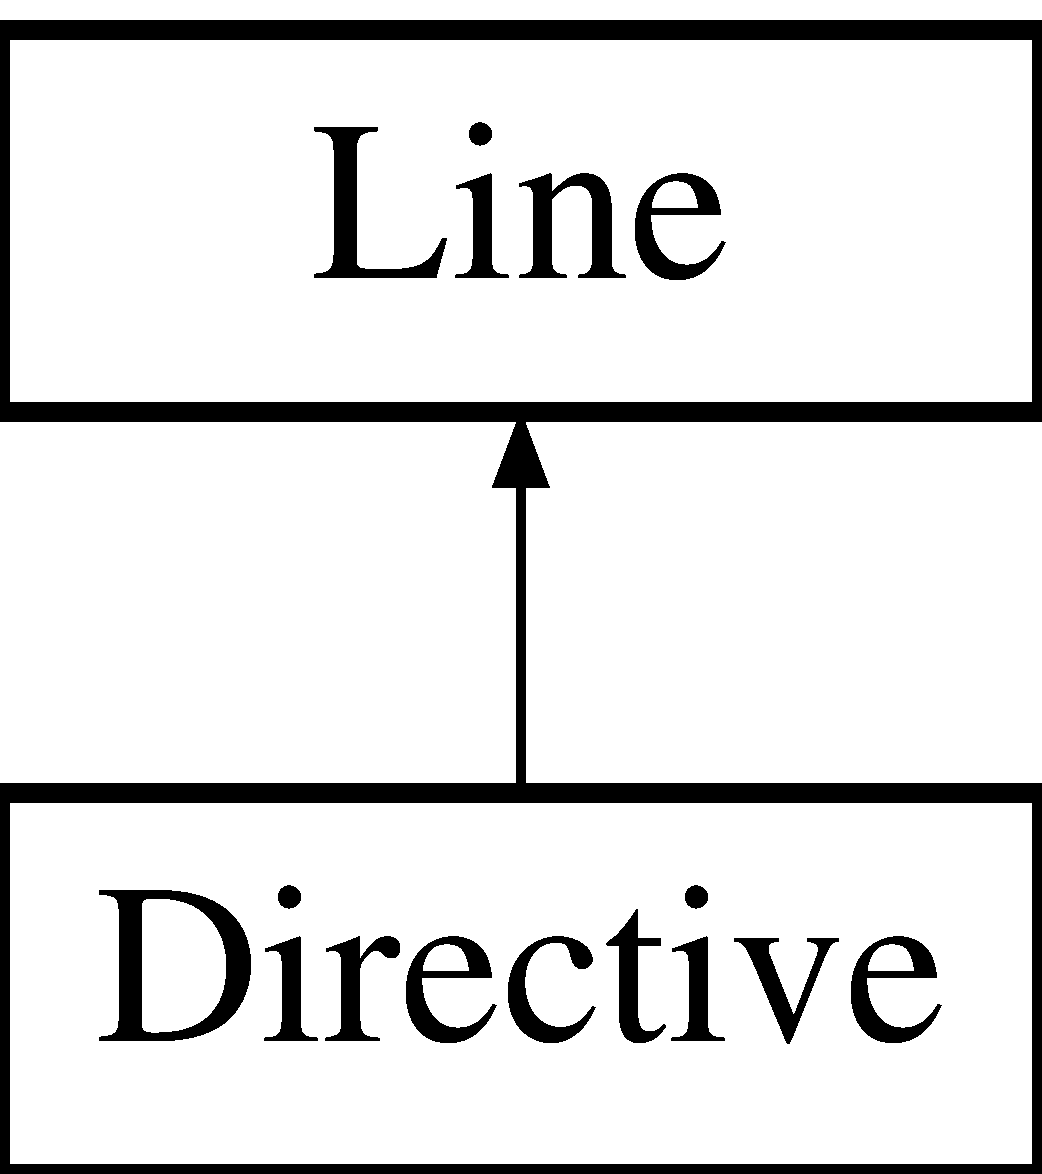
\includegraphics[height=2.000000cm]{class_directive}
\end{center}
\end{figure}
\subsection*{Public Member Functions}
\begin{DoxyCompactItemize}
\item 
\mbox{\Hypertarget{class_directive_a7487120f679e1b4d01843ad6feac7e07}\label{class_directive_a7487120f679e1b4d01843ad6feac7e07}} 
\mbox{\hyperlink{class_directive_a7487120f679e1b4d01843ad6feac7e07}{Directive}} (string)
\begin{DoxyCompactList}\small\item\em Constructor of the \mbox{\hyperlink{class_directive}{Directive}}. \end{DoxyCompactList}\item 
\mbox{\Hypertarget{class_directive_ac2f912e3997d9fed8bc289d77fc06305}\label{class_directive_ac2f912e3997d9fed8bc289d77fc06305}} 
\mbox{\hyperlink{class_directive_ac2f912e3997d9fed8bc289d77fc06305}{Directive}} (string, string)
\begin{DoxyCompactList}\small\item\em Constructor of the \mbox{\hyperlink{class_directive}{Directive}} with directive, content and an boolean. \end{DoxyCompactList}\item 
\mbox{\Hypertarget{class_directive_adbe3bd8e72354bde2b7d809348d0d527}\label{class_directive_adbe3bd8e72354bde2b7d809348d0d527}} 
\mbox{\hyperlink{class_directive_adbe3bd8e72354bde2b7d809348d0d527}{Directive}} (string, string, bool)
\begin{DoxyCompactList}\small\item\em Constructor of the \mbox{\hyperlink{class_directive}{Directive}} with directive, content and an boolean. \end{DoxyCompactList}\item 
\mbox{\Hypertarget{class_directive_aa9a48f09b0472c835ffa366bcff74f51}\label{class_directive_aa9a48f09b0472c835ffa366bcff74f51}} 
virtual \mbox{\hyperlink{class_directive_aa9a48f09b0472c835ffa366bcff74f51}{$\sim$\+Directive}} ()
\begin{DoxyCompactList}\small\item\em Destructor of the \mbox{\hyperlink{class_directive}{Directive}}. \end{DoxyCompactList}\item 
\mbox{\Hypertarget{class_directive_a0d574b0ffc25eb1fbc49032534e7ff44}\label{class_directive_a0d574b0ffc25eb1fbc49032534e7ff44}} 
virtual t\+\_\+\+Line \mbox{\hyperlink{class_directive_a0d574b0ffc25eb1fbc49032534e7ff44}{type\+\_\+line}} ()
\begin{DoxyCompactList}\small\item\em get the type of the line \end{DoxyCompactList}\item 
\mbox{\Hypertarget{class_directive_a2fd56d5580ad7a993782649d7867732f}\label{class_directive_a2fd56d5580ad7a993782649d7867732f}} 
virtual string \mbox{\hyperlink{class_directive_a2fd56d5580ad7a993782649d7867732f}{to\+\_\+string}} ()
\begin{DoxyCompactList}\small\item\em get the string of the \mbox{\hyperlink{class_directive}{Directive}} \end{DoxyCompactList}\item 
\mbox{\Hypertarget{class_directive_aaeb0e95f88f41425718859daeb2116ad}\label{class_directive_aaeb0e95f88f41425718859daeb2116ad}} 
virtual string \mbox{\hyperlink{class_directive_aaeb0e95f88f41425718859daeb2116ad}{get\+\_\+content}} ()
\begin{DoxyCompactList}\small\item\em get the string of the \mbox{\hyperlink{class_directive}{Directive}} \end{DoxyCompactList}\item 
\mbox{\Hypertarget{class_directive_a59b72d2ebc140e3ac0a0d6d789bb5bba}\label{class_directive_a59b72d2ebc140e3ac0a0d6d789bb5bba}} 
virtual void \mbox{\hyperlink{class_directive_a59b72d2ebc140e3ac0a0d6d789bb5bba}{set\+\_\+content}} (string)
\begin{DoxyCompactList}\small\item\em set the string of the \mbox{\hyperlink{class_directive}{Directive}} \end{DoxyCompactList}\item 
\mbox{\Hypertarget{class_directive_ae585a212960cc755c057f85533ddc71e}\label{class_directive_ae585a212960cc755c057f85533ddc71e}} 
bool \mbox{\hyperlink{class_directive_ae585a212960cc755c057f85533ddc71e}{is\+\_\+function}} ()
\begin{DoxyCompactList}\small\item\em return true if the directive indicate a function \end{DoxyCompactList}\item 
\mbox{\Hypertarget{class_directive_a5c3ac59a9d3bc3c16341124482370843}\label{class_directive_a5c3ac59a9d3bc3c16341124482370843}} 
virtual t\+\_\+\+Inst \mbox{\hyperlink{class_directive_a5c3ac59a9d3bc3c16341124482370843}{get\+\_\+type}} ()
\begin{DoxyCompactList}\small\item\em return the type of the instruction \end{DoxyCompactList}\end{DoxyCompactItemize}
\subsection*{Public Attributes}
\begin{DoxyCompactItemize}
\item 
\mbox{\Hypertarget{class_directive_a3e89203d14d83c6ff8da7a1c49b9a60e}\label{class_directive_a3e89203d14d83c6ff8da7a1c49b9a60e}} 
string {\bfseries \+\_\+dir}
\item 
\mbox{\Hypertarget{class_directive_aaeaa71135c6d434d58db763a1e2b70e3}\label{class_directive_aaeaa71135c6d434d58db763a1e2b70e3}} 
string {\bfseries \+\_\+value}
\item 
\mbox{\Hypertarget{class_directive_ae9e02b1ecc6a1b5387f5227959984c1f}\label{class_directive_ae9e02b1ecc6a1b5387f5227959984c1f}} 
bool {\bfseries \+\_\+isfunction}
\end{DoxyCompactItemize}
\subsection*{Additional Inherited Members}


\subsection{Detailed Description}
class representing an \mbox{\hyperlink{class_directive}{Directive}} herited by \mbox{\hyperlink{class_line}{Line}} 

The documentation for this class was generated from the following file\+:\begin{DoxyCompactItemize}
\item 
include/\mbox{\hyperlink{_directive_8h}{Directive.\+h}}\end{DoxyCompactItemize}

\hypertarget{class_function}{}\section{Function Class Reference}
\label{class_function}\index{Function@{Function}}


class representing a \mbox{\hyperlink{class_function}{Function}} in a program  




{\ttfamily \#include $<$Function.\+h$>$}

\subsection*{Public Member Functions}
\begin{DoxyCompactItemize}
\item 
\mbox{\Hypertarget{class_function_ae206568fd4fd4c885e3ccff76345c4e6}\label{class_function_ae206568fd4fd4c885e3ccff76345c4e6}} 
\mbox{\hyperlink{class_function_ae206568fd4fd4c885e3ccff76345c4e6}{Function}} ()
\begin{DoxyCompactList}\small\item\em Constructor of a function. \end{DoxyCompactList}\item 
\mbox{\Hypertarget{class_function_a3b03f7cf0b75d16edebdda1dee1db6fd}\label{class_function_a3b03f7cf0b75d16edebdda1dee1db6fd}} 
\mbox{\hyperlink{class_function_a3b03f7cf0b75d16edebdda1dee1db6fd}{$\sim$\+Function}} ()
\begin{DoxyCompactList}\small\item\em Destructor of a function. \end{DoxyCompactList}\item 
\mbox{\Hypertarget{class_function_a67ffa7175c8ab513df6db299b877ad97}\label{class_function_a67ffa7175c8ab513df6db299b877ad97}} 
void \mbox{\hyperlink{class_function_a67ffa7175c8ab513df6db299b877ad97}{set\+\_\+head}} (\mbox{\hyperlink{class_line}{Line}} $\ast$)
\begin{DoxyCompactList}\small\item\em setter of the head of the function \end{DoxyCompactList}\item 
\mbox{\Hypertarget{class_function_af5b88d118098c4cd6e5e3a4d324b8b48}\label{class_function_af5b88d118098c4cd6e5e3a4d324b8b48}} 
void \mbox{\hyperlink{class_function_af5b88d118098c4cd6e5e3a4d324b8b48}{set\+\_\+end}} (\mbox{\hyperlink{class_line}{Line}} $\ast$)
\begin{DoxyCompactList}\small\item\em setter of the end of the function \end{DoxyCompactList}\item 
\mbox{\Hypertarget{class_function_a1ca74e7cd3f2681ae8ddcc70241fdc29}\label{class_function_a1ca74e7cd3f2681ae8ddcc70241fdc29}} 
\mbox{\hyperlink{class_line}{Line}} $\ast$ \mbox{\hyperlink{class_function_a1ca74e7cd3f2681ae8ddcc70241fdc29}{get\+\_\+head}} ()
\begin{DoxyCompactList}\small\item\em get the head of the function \end{DoxyCompactList}\item 
\mbox{\Hypertarget{class_function_a6789e258845ec7b9d2fd922c6291396d}\label{class_function_a6789e258845ec7b9d2fd922c6291396d}} 
\mbox{\hyperlink{class_basic__block}{Basic\+\_\+block}} $\ast$ \mbox{\hyperlink{class_function_a6789e258845ec7b9d2fd922c6291396d}{get\+\_\+first\+BB}} ()
\begin{DoxyCompactList}\small\item\em get the first BB of the function \end{DoxyCompactList}\item 
\mbox{\Hypertarget{class_function_a319af56932faa6253ebe9db1c821eb4d}\label{class_function_a319af56932faa6253ebe9db1c821eb4d}} 
\mbox{\hyperlink{class_line}{Line}} $\ast$ \mbox{\hyperlink{class_function_a319af56932faa6253ebe9db1c821eb4d}{get\+\_\+end}} ()
\begin{DoxyCompactList}\small\item\em get the ending \mbox{\hyperlink{class_line}{Line}} of the function \end{DoxyCompactList}\item 
\mbox{\Hypertarget{class_function_ade8a6050da83010be473a6581d65a3ce}\label{class_function_ade8a6050da83010be473a6581d65a3ce}} 
void \mbox{\hyperlink{class_function_ade8a6050da83010be473a6581d65a3ce}{display}} ()
\begin{DoxyCompactList}\small\item\em display the function \end{DoxyCompactList}\item 
\mbox{\Hypertarget{class_function_a0b62379b4e18c9440963b54d2e8991b0}\label{class_function_a0b62379b4e18c9440963b54d2e8991b0}} 
int \mbox{\hyperlink{class_function_a0b62379b4e18c9440963b54d2e8991b0}{size}} ()
\begin{DoxyCompactList}\small\item\em get number of Lines of the function \end{DoxyCompactList}\item 
\mbox{\Hypertarget{class_function_acd08be840c48abd3c0c0c20ca4b5192a}\label{class_function_acd08be840c48abd3c0c0c20ca4b5192a}} 
void \mbox{\hyperlink{class_function_acd08be840c48abd3c0c0c20ca4b5192a}{restitution}} (string const)
\begin{DoxyCompactList}\small\item\em restitute the function in a file \end{DoxyCompactList}\item 
\mbox{\Hypertarget{class_function_a5b1550f534becc9b7ae9fe679fc8db10}\label{class_function_a5b1550f534becc9b7ae9fe679fc8db10}} 
void \mbox{\hyperlink{class_function_a5b1550f534becc9b7ae9fe679fc8db10}{add\+\_\+\+BB}} (\mbox{\hyperlink{class_line}{Line}} $\ast$, \mbox{\hyperlink{class_line}{Line}} $\ast$, \mbox{\hyperlink{class_line}{Line}} $\ast$, int)
\begin{DoxyCompactList}\small\item\em creates a new BB with the given start line, end line and branch line and its index, add it to the BB list of this \end{DoxyCompactList}\item 
\mbox{\Hypertarget{class_function_a6094f123294ccbb891fa4145fd5b1b0a}\label{class_function_a6094f123294ccbb891fa4145fd5b1b0a}} 
void \mbox{\hyperlink{class_function_a6094f123294ccbb891fa4145fd5b1b0a}{comput\+\_\+basic\+\_\+block}} ()
\begin{DoxyCompactList}\small\item\em Calculate the basics bolck of the function. \end{DoxyCompactList}\item 
\mbox{\Hypertarget{class_function_a4ddde4ac1ff488dfcbfcaee71f727a48}\label{class_function_a4ddde4ac1ff488dfcbfcaee71f727a48}} 
int \mbox{\hyperlink{class_function_a4ddde4ac1ff488dfcbfcaee71f727a48}{nbr\+\_\+\+BB}} ()
\begin{DoxyCompactList}\small\item\em get the number of Basic block in the function \end{DoxyCompactList}\item 
\mbox{\Hypertarget{class_function_ae11968b8ca5497526e9448b67823d373}\label{class_function_ae11968b8ca5497526e9448b67823d373}} 
\mbox{\hyperlink{class_basic__block}{Basic\+\_\+block}} $\ast$ \mbox{\hyperlink{class_function_ae11968b8ca5497526e9448b67823d373}{get\+\_\+\+BB}} (int)
\begin{DoxyCompactList}\small\item\em get the Basic Block at a position in the BB list \end{DoxyCompactList}\item 
\mbox{\Hypertarget{class_function_a1c8830219ce4306c22a933b17f54cc6f}\label{class_function_a1c8830219ce4306c22a933b17f54cc6f}} 
void \mbox{\hyperlink{class_function_a1c8830219ce4306c22a933b17f54cc6f}{comput\+\_\+label}} ()
\begin{DoxyCompactList}\small\item\em comput labels of the function in list \end{DoxyCompactList}\item 
\mbox{\Hypertarget{class_function_a4b2e9837c4b506b3c7a6d1488d9914d1}\label{class_function_a4b2e9837c4b506b3c7a6d1488d9914d1}} 
\mbox{\hyperlink{class_label}{Label}} $\ast$ \mbox{\hyperlink{class_function_a4b2e9837c4b506b3c7a6d1488d9914d1}{get\+\_\+label}} (int)
\begin{DoxyCompactList}\small\item\em get a specific label of the function \end{DoxyCompactList}\item 
\mbox{\Hypertarget{class_function_a3f3807e12e695ffe23e1ef44edcd262b}\label{class_function_a3f3807e12e695ffe23e1ef44edcd262b}} 
int \mbox{\hyperlink{class_function_a3f3807e12e695ffe23e1ef44edcd262b}{nbr\+\_\+label}} ()
\begin{DoxyCompactList}\small\item\em get the size of the list label \end{DoxyCompactList}\item 
\mbox{\Hypertarget{class_function_ae55c0232d0eced8830daf57293229db8}\label{class_function_ae55c0232d0eced8830daf57293229db8}} 
\mbox{\hyperlink{class_basic__block}{Basic\+\_\+block}} $\ast$ \mbox{\hyperlink{class_function_ae55c0232d0eced8830daf57293229db8}{find\+\_\+label\+\_\+\+BB}} (\mbox{\hyperlink{class_o_p_label}{O\+P\+Label}} $\ast$)
\begin{DoxyCompactList}\small\item\em Get the basic block that starts with a given label (operand) \end{DoxyCompactList}\item 
\mbox{\Hypertarget{class_function_a3c52c8cb82e0137f02771331018b655c}\label{class_function_a3c52c8cb82e0137f02771331018b655c}} 
void \mbox{\hyperlink{class_function_a3c52c8cb82e0137f02771331018b655c}{comput\+\_\+succ\+\_\+pred\+\_\+\+BB}} ()
\begin{DoxyCompactList}\small\item\em Computes the successors and predecessors of each basic block. \end{DoxyCompactList}\item 
\mbox{\Hypertarget{class_function_a9ecf8e774164937c3dfdb989ebe1c866}\label{class_function_a9ecf8e774164937c3dfdb989ebe1c866}} 
void \mbox{\hyperlink{class_function_a9ecf8e774164937c3dfdb989ebe1c866}{compute\+\_\+dom}} ()
\begin{DoxyCompactList}\small\item\em computes dominators for each basic block \end{DoxyCompactList}\item 
\mbox{\Hypertarget{class_function_a20c7a6df3cb39a134fe5dcc9749bdf2e}\label{class_function_a20c7a6df3cb39a134fe5dcc9749bdf2e}} 
void \mbox{\hyperlink{class_function_a20c7a6df3cb39a134fe5dcc9749bdf2e}{compute\+\_\+loops}} ()
\begin{DoxyCompactList}\small\item\em computes loops inside the function \end{DoxyCompactList}\item 
\mbox{\Hypertarget{class_function_a93ab02fb20a2d5d573f930a111db84f5}\label{class_function_a93ab02fb20a2d5d573f930a111db84f5}} 
void \mbox{\hyperlink{class_function_a93ab02fb20a2d5d573f930a111db84f5}{display\+\_\+loops}} ()
\begin{DoxyCompactList}\small\item\em show the loops of the function \end{DoxyCompactList}\item 
\mbox{\Hypertarget{class_function_a21b614fb69692ba00240831c8fe8beb9}\label{class_function_a21b614fb69692ba00240831c8fe8beb9}} 
void \mbox{\hyperlink{class_function_a21b614fb69692ba00240831c8fe8beb9}{compute\+\_\+live\+\_\+var}} ()
\begin{DoxyCompactList}\small\item\em computes alive variables for each basic block \end{DoxyCompactList}\item 
\mbox{\Hypertarget{class_function_a970520528e3f91736849ca773d6e6bff}\label{class_function_a970520528e3f91736849ca773d6e6bff}} 
void \mbox{\hyperlink{class_function_a970520528e3f91736849ca773d6e6bff}{show\+\_\+live\+\_\+var}} ()
\begin{DoxyCompactList}\small\item\em display alive variables for each basic block \end{DoxyCompactList}\item 
\mbox{\Hypertarget{class_function_aaa0d06640a5075c416106a88bd9a833a}\label{class_function_aaa0d06640a5075c416106a88bd9a833a}} 
void \mbox{\hyperlink{class_function_aaa0d06640a5075c416106a88bd9a833a}{test}} ()
\begin{DoxyCompactList}\small\item\em method to perform some test, usefull for testing methods on basic blocks \end{DoxyCompactList}\end{DoxyCompactItemize}


\subsection{Detailed Description}
class representing a \mbox{\hyperlink{class_function}{Function}} in a program 

The documentation for this class was generated from the following file\+:\begin{DoxyCompactItemize}
\item 
include/\mbox{\hyperlink{_function_8h}{Function.\+h}}\end{DoxyCompactItemize}

\hypertarget{class_instruction}{}\section{Instruction Class Reference}
\label{class_instruction}\index{Instruction@{Instruction}}


class representing an instruction which herited by \mbox{\hyperlink{class_line}{Line}}  




{\ttfamily \#include $<$Instruction.\+h$>$}

Inheritance diagram for Instruction\+:\begin{figure}[H]
\begin{center}
\leavevmode
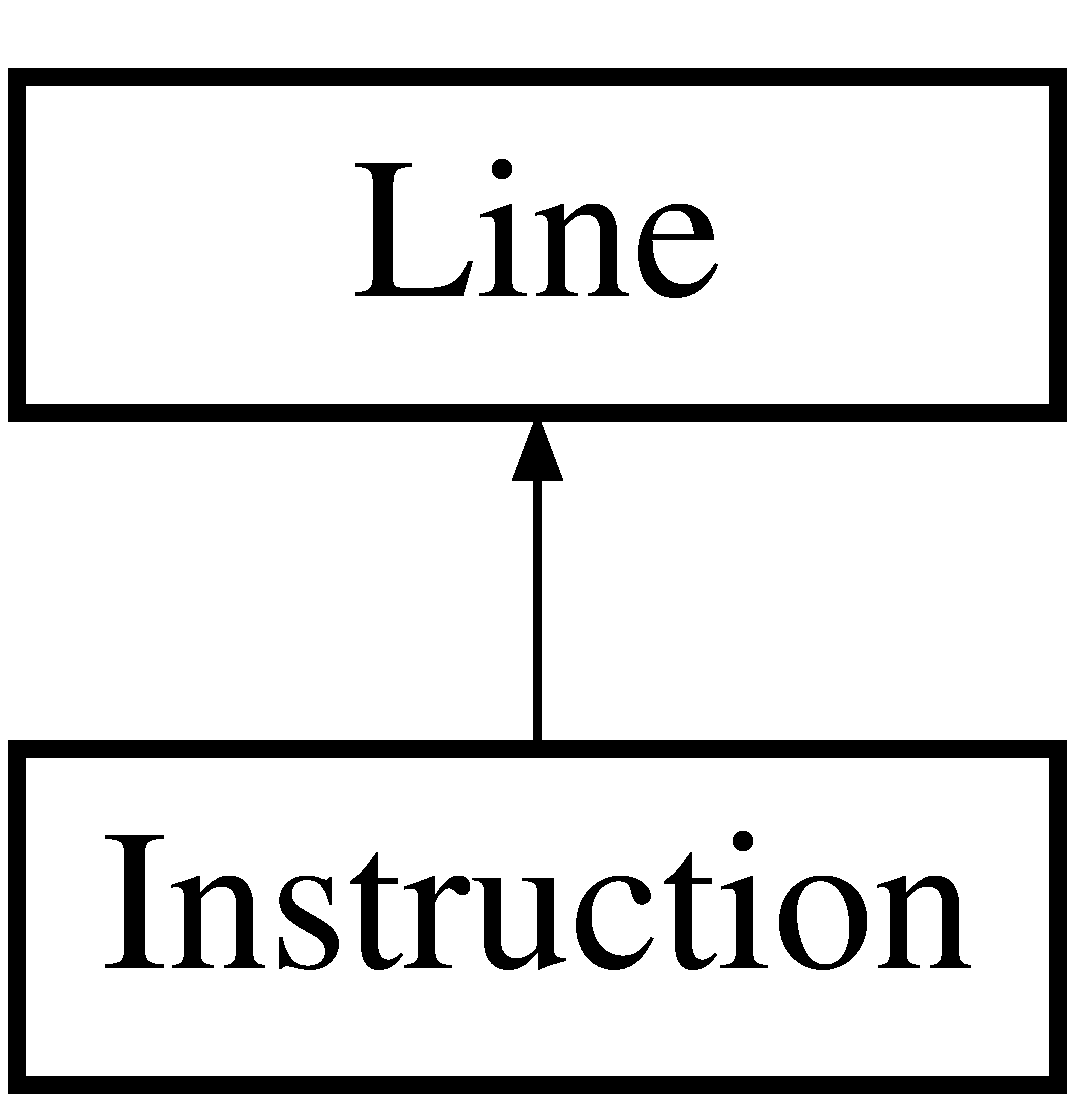
\includegraphics[height=2.000000cm]{class_instruction}
\end{center}
\end{figure}
\subsection*{Public Member Functions}
\begin{DoxyCompactItemize}
\item 
void \mbox{\hyperlink{class_instruction_a0bae837f79caa83504ad14172bf6addf}{display}} (void)
\begin{DoxyCompactList}\small\item\em get the Opcode value accessor of the opcode \end{DoxyCompactList}\item 
\mbox{\Hypertarget{class_instruction_a5b258bf1dfb9f6fa2fff0af0e7c211d8}\label{class_instruction_a5b258bf1dfb9f6fa2fff0af0e7c211d8}} 
virtual string \mbox{\hyperlink{class_instruction_a5b258bf1dfb9f6fa2fff0af0e7c211d8}{get\+\_\+content}} ()
\begin{DoxyCompactList}\small\item\em get the string of the instruction \end{DoxyCompactList}\item 
\mbox{\Hypertarget{class_instruction_aab8e6a16b8bab5ca90b554086cc3c825}\label{class_instruction_aab8e6a16b8bab5ca90b554086cc3c825}} 
bool \mbox{\hyperlink{class_instruction_aab8e6a16b8bab5ca90b554086cc3c825}{is\+\_\+branch}} ()
\begin{DoxyCompactList}\small\item\em test if the instruction is a branch or jump instruction \end{DoxyCompactList}\item 
\mbox{\Hypertarget{class_instruction_ab2a6352a09271a588f6930852a361f67}\label{class_instruction_ab2a6352a09271a588f6930852a361f67}} 
bool \mbox{\hyperlink{class_instruction_ab2a6352a09271a588f6930852a361f67}{is\+\_\+call}} ()
\begin{DoxyCompactList}\small\item\em test if the instruction is a call \end{DoxyCompactList}\item 
\mbox{\Hypertarget{class_instruction_a1b607074554bc160142786c125bde530}\label{class_instruction_a1b607074554bc160142786c125bde530}} 
bool \mbox{\hyperlink{class_instruction_a1b607074554bc160142786c125bde530}{is\+\_\+cond\+\_\+branch}} ()
\begin{DoxyCompactList}\small\item\em test if the instruction is a conditionnal branch \end{DoxyCompactList}\item 
\mbox{\Hypertarget{class_instruction_affdf2382cd36277fb4427cd3b07c1402}\label{class_instruction_affdf2382cd36277fb4427cd3b07c1402}} 
bool \mbox{\hyperlink{class_instruction_affdf2382cd36277fb4427cd3b07c1402}{is\+\_\+indirect\+\_\+branch}} ()
\begin{DoxyCompactList}\small\item\em test if the instruction a branch and the target adress is in a register \end{DoxyCompactList}\item 
\mbox{\Hypertarget{class_instruction_aa32973fb1e9e24659095e4795c153c8a}\label{class_instruction_aa32973fb1e9e24659095e4795c153c8a}} 
\mbox{\hyperlink{class_o_p_label}{O\+P\+Label}} $\ast$ \mbox{\hyperlink{class_instruction_aa32973fb1e9e24659095e4795c153c8a}{get\+\_\+op\+\_\+label}} ()
\begin{DoxyCompactList}\small\item\em get the label operand of the instruction, if any \end{DoxyCompactList}\item 
\mbox{\Hypertarget{class_instruction_adb43e7019987daebb3970335aba695cc}\label{class_instruction_adb43e7019987daebb3970335aba695cc}} 
\mbox{\hyperlink{class_o_p_register}{O\+P\+Register}} $\ast$ \mbox{\hyperlink{class_instruction_adb43e7019987daebb3970335aba695cc}{get\+\_\+reg\+\_\+dst}} ()
\begin{DoxyCompactList}\small\item\em get the register destination of the instruction, if any \end{DoxyCompactList}\item 
\mbox{\Hypertarget{class_instruction_ac353a6ad2b3f3b1aee179d5910b5127b}\label{class_instruction_ac353a6ad2b3f3b1aee179d5910b5127b}} 
\mbox{\hyperlink{class_o_p_register}{O\+P\+Register}} $\ast$ \mbox{\hyperlink{class_instruction_ac353a6ad2b3f3b1aee179d5910b5127b}{get\+\_\+reg\+\_\+src1}} ()
\begin{DoxyCompactList}\small\item\em get the first register source of the instruction \end{DoxyCompactList}\item 
\mbox{\Hypertarget{class_instruction_a0eb007b1b0a038610e71a58af3bb6438}\label{class_instruction_a0eb007b1b0a038610e71a58af3bb6438}} 
\mbox{\hyperlink{class_o_p_register}{O\+P\+Register}} $\ast$ \mbox{\hyperlink{class_instruction_a0eb007b1b0a038610e71a58af3bb6438}{get\+\_\+reg\+\_\+src2}} ()
\begin{DoxyCompactList}\small\item\em get the second register source of the instruction \end{DoxyCompactList}\item 
\mbox{\Hypertarget{class_instruction_a14c5f91c242a5b58eda9f123ad331cbe}\label{class_instruction_a14c5f91c242a5b58eda9f123ad331cbe}} 
int \mbox{\hyperlink{class_instruction_a14c5f91c242a5b58eda9f123ad331cbe}{get\+\_\+index}} ()
\begin{DoxyCompactList}\small\item\em get the index of instruction \end{DoxyCompactList}\item 
\mbox{\Hypertarget{class_instruction_a93d5d6186afcf358c5a21f4c57a0d72e}\label{class_instruction_a93d5d6186afcf358c5a21f4c57a0d72e}} 
\mbox{\hyperlink{class_instruction}{Instruction}} $\ast$ \mbox{\hyperlink{class_instruction_a93d5d6186afcf358c5a21f4c57a0d72e}{get\+\_\+next}} ()
\begin{DoxyCompactList}\small\item\em get the successor of the \mbox{\hyperlink{class_instruction}{Instruction}} (given by the schedule of instruction in its basic block) \end{DoxyCompactList}\item 
\mbox{\Hypertarget{class_instruction_afd6f27235469926b1e7979220495a6f0}\label{class_instruction_afd6f27235469926b1e7979220495a6f0}} 
\mbox{\hyperlink{class_instruction}{Instruction}} $\ast$ \mbox{\hyperlink{class_instruction_afd6f27235469926b1e7979220495a6f0}{get\+\_\+prev}} ()
\begin{DoxyCompactList}\small\item\em get the predecessor of the \mbox{\hyperlink{class_instruction}{Instruction}} (given by the schedule of instruction in its basic block) \end{DoxyCompactList}\item 
bool \mbox{\hyperlink{class_instruction_ae5d54f535adab416c53eb0ff6a438804}{is\+\_\+dep\+\_\+\+R\+A\+W1}} (\mbox{\hyperlink{class_instruction}{Instruction}} $\ast$i2)
\begin{DoxyCompactList}\small\item\em return if there is dependance R\+AW between the current instruction and the first source operand of i2 ~\newline
 \end{DoxyCompactList}\item 
bool \mbox{\hyperlink{class_instruction_aa28ae5f427ee02c96466f1ac68060f87}{is\+\_\+dep\+\_\+\+R\+A\+W2}} (\mbox{\hyperlink{class_instruction}{Instruction}} $\ast$i2)
\begin{DoxyCompactList}\small\item\em return if there is dependance R\+AW between the current instruction and the second source operand of i2 ~\newline
 \end{DoxyCompactList}\item 
bool \mbox{\hyperlink{class_instruction_a36c0faedd74af14b403ba7063af5d07f}{is\+\_\+dep\+\_\+\+W\+A\+R1}} (\mbox{\hyperlink{class_instruction}{Instruction}} $\ast$i2)
\begin{DoxyCompactList}\small\item\em test if there is dependance W\+AR between the first source operande of the current instruction if any and the destination register operande i2 if any \end{DoxyCompactList}\item 
bool \mbox{\hyperlink{class_instruction_a04471df677984f67ec13de88f55e3703}{is\+\_\+dep\+\_\+\+W\+A\+R2}} (\mbox{\hyperlink{class_instruction}{Instruction}} $\ast$i2)
\begin{DoxyCompactList}\small\item\em test if there is dependance W\+AR between the second source operande of the current instruction if any and the destination register operande i2 if any ~\newline
 \end{DoxyCompactList}\item 
bool \mbox{\hyperlink{class_instruction_a30c159faa5c462bb2c7ae7562c9c8254}{is\+\_\+dep\+\_\+\+W\+AW}} (\mbox{\hyperlink{class_instruction}{Instruction}} $\ast$i2)
\begin{DoxyCompactList}\small\item\em get the information if there is dependance W\+AW between the current instruction and i2 ~\newline
 \end{DoxyCompactList}\item 
bool \mbox{\hyperlink{class_instruction_a28526bda91b964d7fd81f85cee02c624}{is\+\_\+dep\+\_\+\+M\+EM}} (\mbox{\hyperlink{class_instruction}{Instruction}} $\ast$i2)
\begin{DoxyCompactList}\small\item\em test if there is dependance M\+E\+M\+D\+EP between the current instruction and i2 ~\newline
 \end{DoxyCompactList}\item 
\mbox{\Hypertarget{class_instruction_ab8f6e21bc94df2198678a3cdbcfaa12e}\label{class_instruction_ab8f6e21bc94df2198678a3cdbcfaa12e}} 
void \mbox{\hyperlink{class_instruction_ab8f6e21bc94df2198678a3cdbcfaa12e}{set\+\_\+link\+\_\+succ\+\_\+pred}} (\mbox{\hyperlink{class_instruction}{Instruction}} $\ast$)
\begin{DoxyCompactList}\small\item\em set the parameter as successor and this as predecessor of the parameter \end{DoxyCompactList}\item 
\mbox{\Hypertarget{class_instruction_a3121dad231e2b4c27ac3cae6c8627ece}\label{class_instruction_a3121dad231e2b4c27ac3cae6c8627ece}} 
void \mbox{\hyperlink{class_instruction_a3121dad231e2b4c27ac3cae6c8627ece}{add\+\_\+pred\+\_\+dep}} (\mbox{\hyperlink{structdep}{dep}} $\ast$)
\begin{DoxyCompactList}\small\item\em add a dependance with a predecessor instruction to the dependance type list \end{DoxyCompactList}\item 
\mbox{\Hypertarget{class_instruction_ab32531f8dd490b1c8396b6723f87bfae}\label{class_instruction_ab32531f8dd490b1c8396b6723f87bfae}} 
\mbox{\hyperlink{structdep}{dep}} $\ast$ \mbox{\hyperlink{class_instruction_ab32531f8dd490b1c8396b6723f87bfae}{get\+\_\+pred\+\_\+dep}} (int i)
\begin{DoxyCompactList}\small\item\em get the dependance type with the ith predecessor instruction of the current instruction \end{DoxyCompactList}\item 
\mbox{\Hypertarget{class_instruction_acefc258dbcf45c19136dc86e47a82c0e}\label{class_instruction_acefc258dbcf45c19136dc86e47a82c0e}} 
void \mbox{\hyperlink{class_instruction_acefc258dbcf45c19136dc86e47a82c0e}{add\+\_\+succ\+\_\+dep}} (\mbox{\hyperlink{structdep}{dep}} $\ast$)
\begin{DoxyCompactList}\small\item\em add a dependance with a successor to list of the dependance type of successors \end{DoxyCompactList}\item 
\mbox{\Hypertarget{class_instruction_ad3bb47ea5f9e4b975e0191d6c96ffc30}\label{class_instruction_ad3bb47ea5f9e4b975e0191d6c96ffc30}} 
\mbox{\hyperlink{structdep}{dep}} $\ast$ \mbox{\hyperlink{class_instruction_ad3bb47ea5f9e4b975e0191d6c96ffc30}{get\+\_\+succ\+\_\+dep}} (int i)
\begin{DoxyCompactList}\small\item\em get the ieme dependance type with successors from successor dependance type list of the current instruction \end{DoxyCompactList}\item 
\mbox{\Hypertarget{class_instruction_ab2d8c29efa78ec3c1a70f154a8c2f068}\label{class_instruction_ab2d8c29efa78ec3c1a70f154a8c2f068}} 
int \mbox{\hyperlink{class_instruction_ab2d8c29efa78ec3c1a70f154a8c2f068}{get\+\_\+nb\+\_\+succ}} ()
\begin{DoxyCompactList}\small\item\em get the number of successor (dependance) of the \mbox{\hyperlink{class_instruction}{Instruction}} \end{DoxyCompactList}\item 
\mbox{\Hypertarget{class_instruction_a9e56e8e2c857abc409f27af9f80f9595}\label{class_instruction_a9e56e8e2c857abc409f27af9f80f9595}} 
int \mbox{\hyperlink{class_instruction_a9e56e8e2c857abc409f27af9f80f9595}{get\+\_\+nb\+\_\+pred}} ()
\begin{DoxyCompactList}\small\item\em get the number of predecessor (dependance) of the \mbox{\hyperlink{class_instruction}{Instruction}} \end{DoxyCompactList}\item 
\mbox{\Hypertarget{class_instruction_af489e680ae3c69fd12b0a23e959172e5}\label{class_instruction_af489e680ae3c69fd12b0a23e959172e5}} 
void \mbox{\hyperlink{class_instruction_af489e680ae3c69fd12b0a23e959172e5}{print\+\_\+succ\+\_\+dep}} ()
\begin{DoxyCompactList}\small\item\em print the dependance of this with instructions denoted by their index and the dependance type \end{DoxyCompactList}\item 
\mbox{\Hypertarget{class_instruction_a786e43bcd16d16a4db7c8a665c4d68af}\label{class_instruction_a786e43bcd16d16a4db7c8a665c4d68af}} 
void \mbox{\hyperlink{class_instruction_a786e43bcd16d16a4db7c8a665c4d68af}{reset\+\_\+pred\+\_\+succ\+\_\+dep}} ()
\begin{DoxyCompactList}\small\item\em reset succ and pred dependances of this \end{DoxyCompactList}\item 
\mbox{\Hypertarget{class_instruction_a2c6f13ddda889e4e2b8b69897de6b733}\label{class_instruction_a2c6f13ddda889e4e2b8b69897de6b733}} 
list$<$ \mbox{\hyperlink{structdep}{dep}} $\ast$ $>$\+::iterator {\bfseries succ\+\_\+begin} ()
\item 
\mbox{\Hypertarget{class_instruction_a0800ca0afbbc783b57170d981d406fb6}\label{class_instruction_a0800ca0afbbc783b57170d981d406fb6}} 
list$<$ \mbox{\hyperlink{structdep}{dep}} $\ast$ $>$\+::iterator {\bfseries succ\+\_\+end} ()
\item 
\mbox{\Hypertarget{class_instruction_a300e014a1136068872d235d3e41d5376}\label{class_instruction_a300e014a1136068872d235d3e41d5376}} 
list$<$ \mbox{\hyperlink{structdep}{dep}} $\ast$ $>$\+::iterator {\bfseries pred\+\_\+begin} ()
\item 
\mbox{\Hypertarget{class_instruction_a0c14cd69b30373678261f8aa0da029ab}\label{class_instruction_a0c14cd69b30373678261f8aa0da029ab}} 
list$<$ \mbox{\hyperlink{structdep}{dep}} $\ast$ $>$\+::iterator {\bfseries pred\+\_\+end} ()
\item 
\mbox{\Hypertarget{class_instruction_a2222ad40481088c12a38c5f340bcd86b}\label{class_instruction_a2222ad40481088c12a38c5f340bcd86b}} 
bool \mbox{\hyperlink{class_instruction_a2222ad40481088c12a38c5f340bcd86b}{is\+\_\+nop}} ()
\begin{DoxyCompactList}\small\item\em test if the instruction a branch and the target adress is in a register \end{DoxyCompactList}\item 
\mbox{\Hypertarget{class_instruction_a1c79865faf9baa4d70edf81e956d952d}\label{class_instruction_a1c79865faf9baa4d70edf81e956d952d}} 
bool \mbox{\hyperlink{class_instruction_a1c79865faf9baa4d70edf81e956d952d}{is\+\_\+mem}} ()
\begin{DoxyCompactList}\small\item\em test if the instruction is a memory access \end{DoxyCompactList}\item 
\mbox{\Hypertarget{class_instruction_aee32f4bb91480afc74375beb139af4d6}\label{class_instruction_aee32f4bb91480afc74375beb139af4d6}} 
bool \mbox{\hyperlink{class_instruction_aee32f4bb91480afc74375beb139af4d6}{is\+\_\+mem\+\_\+load}} ()
\begin{DoxyCompactList}\small\item\em test if the instruction is a memory access that reads a value \end{DoxyCompactList}\item 
\mbox{\Hypertarget{class_instruction_a4455144397d239eb61bcfa2b0e16bf67}\label{class_instruction_a4455144397d239eb61bcfa2b0e16bf67}} 
bool \mbox{\hyperlink{class_instruction_a4455144397d239eb61bcfa2b0e16bf67}{is\+\_\+mem\+\_\+store}} ()
\begin{DoxyCompactList}\small\item\em test if the instruction is a memory access that writes a value \end{DoxyCompactList}\item 
\mbox{\Hypertarget{class_instruction_a1195d03eb4ff6024b20cd2cec1c8a1e0}\label{class_instruction_a1195d03eb4ff6024b20cd2cec1c8a1e0}} 
t\+\_\+\+Operator \mbox{\hyperlink{class_instruction_a1195d03eb4ff6024b20cd2cec1c8a1e0}{get\+\_\+opcode}} ()
\begin{DoxyCompactList}\small\item\em get the Opcode \end{DoxyCompactList}\item 
\mbox{\Hypertarget{class_instruction_aeba180e03a3ac7f7ecba7635d454566f}\label{class_instruction_aeba180e03a3ac7f7ecba7635d454566f}} 
string \mbox{\hyperlink{class_instruction_aeba180e03a3ac7f7ecba7635d454566f}{string\+\_\+opcode}} ()
\begin{DoxyCompactList}\small\item\em get the string Opcode value accessor of the string opcode \end{DoxyCompactList}\item 
\mbox{\Hypertarget{class_instruction_a49524f35c4ade25c663d798e3a5df2cb}\label{class_instruction_a49524f35c4ade25c663d798e3a5df2cb}} 
void \mbox{\hyperlink{class_instruction_a49524f35c4ade25c663d798e3a5df2cb}{set\+\_\+opcode}} (t\+\_\+\+Operator newop)
\begin{DoxyCompactList}\small\item\em set the opcode value setter of the opcode \end{DoxyCompactList}\item 
\mbox{\Hypertarget{class_instruction_a86e8d9627ad78884d75481693a6196ef}\label{class_instruction_a86e8d9627ad78884d75481693a6196ef}} 
t\+\_\+\+Format \mbox{\hyperlink{class_instruction_a86e8d9627ad78884d75481693a6196ef}{get\+\_\+format}} ()
\begin{DoxyCompactList}\small\item\em get the format of the \mbox{\hyperlink{class_instruction}{Instruction}} accessor of the format (see \mbox{\hyperlink{_enum__type_8h_source}{Enum\+\_\+type.\+h}}) \end{DoxyCompactList}\item 
\mbox{\Hypertarget{class_instruction_ae619398c5531b1f2042fb4caa893cdee}\label{class_instruction_ae619398c5531b1f2042fb4caa893cdee}} 
virtual t\+\_\+\+Inst \mbox{\hyperlink{class_instruction_ae619398c5531b1f2042fb4caa893cdee}{get\+\_\+type}} ()
\begin{DoxyCompactList}\small\item\em get the Type of the \mbox{\hyperlink{class_instruction}{Instruction}} accessor of the Type (see \mbox{\hyperlink{_enum__type_8h_source}{Enum\+\_\+type.\+h}}) \end{DoxyCompactList}\item 
\mbox{\Hypertarget{class_instruction_ac2988d2fb858b720e009da03120ae4c7}\label{class_instruction_ac2988d2fb858b720e009da03120ae4c7}} 
int \mbox{\hyperlink{class_instruction_ac2988d2fb858b720e009da03120ae4c7}{get\+\_\+latency}} ()
\begin{DoxyCompactList}\small\item\em return the latency of the instruction \end{DoxyCompactList}\item 
\mbox{\Hypertarget{class_instruction_adcab5ded0016e613826be14514abbcc8}\label{class_instruction_adcab5ded0016e613826be14514abbcc8}} 
virtual t\+\_\+\+Line \mbox{\hyperlink{class_instruction_adcab5ded0016e613826be14514abbcc8}{type\+\_\+line}} ()
\begin{DoxyCompactList}\small\item\em get the type of the line \end{DoxyCompactList}\item 
\mbox{\Hypertarget{class_instruction_aed87de5e9259f4f15dc885425528f1fe}\label{class_instruction_aed87de5e9259f4f15dc885425528f1fe}} 
virtual string \mbox{\hyperlink{class_instruction_aed87de5e9259f4f15dc885425528f1fe}{to\+\_\+string}} ()
\begin{DoxyCompactList}\small\item\em get the name string instruction \end{DoxyCompactList}\item 
\mbox{\Hypertarget{class_instruction_aec1a1ab575287b532fb8d43cfa364e30}\label{class_instruction_aec1a1ab575287b532fb8d43cfa364e30}} 
virtual void \mbox{\hyperlink{class_instruction_aec1a1ab575287b532fb8d43cfa364e30}{set\+\_\+content}} (string)
\begin{DoxyCompactList}\small\item\em set the string of the instruction \end{DoxyCompactList}\item 
\mbox{\Hypertarget{class_instruction_a2d2d966c6269e1e0dbfbeb8aabafeeb4}\label{class_instruction_a2d2d966c6269e1e0dbfbeb8aabafeeb4}} 
string \mbox{\hyperlink{class_instruction_a2d2d966c6269e1e0dbfbeb8aabafeeb4}{string\+\_\+form}} ()
\begin{DoxyCompactList}\small\item\em set the string format \end{DoxyCompactList}\item 
\mbox{\Hypertarget{class_instruction_ac2d81dcf8ddd82e31262c7adb1a0df69}\label{class_instruction_ac2d81dcf8ddd82e31262c7adb1a0df69}} 
string \mbox{\hyperlink{class_instruction_ac2d81dcf8ddd82e31262c7adb1a0df69}{string\+\_\+type}} ()
\begin{DoxyCompactList}\small\item\em set the string Type of instruction \end{DoxyCompactList}\item 
\mbox{\Hypertarget{class_instruction_af1608cfea660c46e8a8b4bbac948406a}\label{class_instruction_af1608cfea660c46e8a8b4bbac948406a}} 
void \mbox{\hyperlink{class_instruction_af1608cfea660c46e8a8b4bbac948406a}{set\+\_\+index}} (int)
\begin{DoxyCompactList}\small\item\em set the index of instruction \end{DoxyCompactList}\item 
\mbox{\Hypertarget{class_instruction_a69d2992a0eb1fbe5fb6a38b52e13a804}\label{class_instruction_a69d2992a0eb1fbe5fb6a38b52e13a804}} 
void \mbox{\hyperlink{class_instruction_a69d2992a0eb1fbe5fb6a38b52e13a804}{set\+\_\+prev}} (\mbox{\hyperlink{class_instruction}{Instruction}} $\ast$)
\begin{DoxyCompactList}\small\item\em setter of the predecessor of the \mbox{\hyperlink{class_instruction}{Instruction}} \end{DoxyCompactList}\item 
\mbox{\Hypertarget{class_instruction_a2fb436e52a0cc89e7ec08bf0e105bba3}\label{class_instruction_a2fb436e52a0cc89e7ec08bf0e105bba3}} 
void \mbox{\hyperlink{class_instruction_a2fb436e52a0cc89e7ec08bf0e105bba3}{set\+\_\+next}} (\mbox{\hyperlink{class_instruction}{Instruction}} $\ast$)
\begin{DoxyCompactList}\small\item\em set the successor of the \mbox{\hyperlink{class_instruction}{Instruction}} \end{DoxyCompactList}\item 
t\+\_\+\+Dep \mbox{\hyperlink{class_instruction_ac8d86b800140a08cb03d82f83f363fa4}{is\+\_\+dependant}} (\mbox{\hyperlink{class_instruction}{Instruction}} $\ast$i2)
\begin{DoxyCompactList}\small\item\em get the dependance between the current instruction and i2 \end{DoxyCompactList}\item 
bool \mbox{\hyperlink{class_instruction_a4c902c5a8fdc8c8841ec24f389605fd5}{is\+\_\+dep\+\_\+\+R\+AW}} (\mbox{\hyperlink{class_instruction}{Instruction}} $\ast$i2)
\begin{DoxyCompactList}\small\item\em get the information if there is dependance R\+AW between the current instruction and i2 ~\newline
 \end{DoxyCompactList}\item 
bool \mbox{\hyperlink{class_instruction_ae79b239c6ab30a15064b5a00944ad65a}{is\+\_\+dep\+\_\+\+W\+AR}} (\mbox{\hyperlink{class_instruction}{Instruction}} $\ast$i2)
\begin{DoxyCompactList}\small\item\em get the information if there is dependance W\+AR between the current instruction and i2 ~\newline
 \end{DoxyCompactList}\item 
int \mbox{\hyperlink{class_instruction_a044a281355f25375a7765f24bdf614f3}{get\+\_\+nb\+Op}} ()
\begin{DoxyCompactList}\small\item\em get the number of operand ~\newline
 \end{DoxyCompactList}\item 
\mbox{\Hypertarget{class_instruction_a6ff2d531dffa43d3db22194459336d33}\label{class_instruction_a6ff2d531dffa43d3db22194459336d33}} 
void \mbox{\hyperlink{class_instruction_a6ff2d531dffa43d3db22194459336d33}{set\+\_\+number\+\_\+oper}} (int)
\begin{DoxyCompactList}\small\item\em set the number of operand \end{DoxyCompactList}\item 
\mbox{\Hypertarget{class_instruction_a055c483afc0512b68f6211fdbb6774ba}\label{class_instruction_a055c483afc0512b68f6211fdbb6774ba}} 
\mbox{\hyperlink{class_instruction_a055c483afc0512b68f6211fdbb6774ba}{Instruction}} (string, t\+\_\+\+Operator, t\+\_\+\+Inst, \mbox{\hyperlink{class_operand}{Operand}} $\ast$, \mbox{\hyperlink{class_operand}{Operand}} $\ast$, \mbox{\hyperlink{class_operand}{Operand}} $\ast$)
\begin{DoxyCompactList}\small\item\em Constructor of the class instruction. \end{DoxyCompactList}\item 
\mbox{\Hypertarget{class_instruction_a2f1ed1606d4090b8a4c255e3af9e34c8}\label{class_instruction_a2f1ed1606d4090b8a4c255e3af9e34c8}} 
\mbox{\hyperlink{class_instruction_a2f1ed1606d4090b8a4c255e3af9e34c8}{Instruction}} (t\+\_\+\+Operator, \mbox{\hyperlink{class_operand}{Operand}} $\ast$, \mbox{\hyperlink{class_operand}{Operand}} $\ast$, \mbox{\hyperlink{class_operand}{Operand}} $\ast$)
\begin{DoxyCompactList}\small\item\em Constructor with 3 Operands of the class instruction. \end{DoxyCompactList}\item 
\mbox{\Hypertarget{class_instruction_a0b1ed4432c9c5823ee9e522c7d11bb5f}\label{class_instruction_a0b1ed4432c9c5823ee9e522c7d11bb5f}} 
\mbox{\hyperlink{class_instruction_a0b1ed4432c9c5823ee9e522c7d11bb5f}{Instruction}} (t\+\_\+\+Operator, \mbox{\hyperlink{class_operand}{Operand}} $\ast$, \mbox{\hyperlink{class_operand}{Operand}} $\ast$)
\begin{DoxyCompactList}\small\item\em Constructor with 2 Operands of the class instruction. \end{DoxyCompactList}\item 
\mbox{\Hypertarget{class_instruction_a6ae2a4dd83500f9d538a653823161b1c}\label{class_instruction_a6ae2a4dd83500f9d538a653823161b1c}} 
\mbox{\hyperlink{class_instruction_a6ae2a4dd83500f9d538a653823161b1c}{Instruction}} (t\+\_\+\+Operator, \mbox{\hyperlink{class_operand}{Operand}} $\ast$)
\begin{DoxyCompactList}\small\item\em Constructor with 1 \mbox{\hyperlink{class_operand}{Operand}} of the class instruction. \end{DoxyCompactList}\item 
\mbox{\Hypertarget{class_instruction_ab2d989cc18e9bf0eeee194a7614514fa}\label{class_instruction_ab2d989cc18e9bf0eeee194a7614514fa}} 
\mbox{\hyperlink{class_instruction_ab2d989cc18e9bf0eeee194a7614514fa}{Instruction}} (t\+\_\+\+Operator)
\begin{DoxyCompactList}\small\item\em Constructor without Operands of the class instruction. \end{DoxyCompactList}\item 
\mbox{\Hypertarget{class_instruction_a3f1031e811b710787678f8faf8cc9672}\label{class_instruction_a3f1031e811b710787678f8faf8cc9672}} 
virtual \mbox{\hyperlink{class_instruction_a3f1031e811b710787678f8faf8cc9672}{$\sim$\+Instruction}} ()
\begin{DoxyCompactList}\small\item\em Destructor of the class instruction. \end{DoxyCompactList}\end{DoxyCompactItemize}
\subsection*{Additional Inherited Members}


\subsection{Detailed Description}
class representing an instruction which herited by \mbox{\hyperlink{class_line}{Line}} 

\subsection{Member Function Documentation}
\mbox{\Hypertarget{class_instruction_a0bae837f79caa83504ad14172bf6addf}\label{class_instruction_a0bae837f79caa83504ad14172bf6addf}} 
\index{Instruction@{Instruction}!display@{display}}
\index{display@{display}!Instruction@{Instruction}}
\subsubsection{\texorpdfstring{display()}{display()}}
{\footnotesize\ttfamily void Instruction\+::display (\begin{DoxyParamCaption}\item[{void}]{ }\end{DoxyParamCaption})}



get the Opcode value accessor of the opcode 

display the instruction \mbox{\Hypertarget{class_instruction_a044a281355f25375a7765f24bdf614f3}\label{class_instruction_a044a281355f25375a7765f24bdf614f3}} 
\index{Instruction@{Instruction}!get\+\_\+nb\+Op@{get\+\_\+nb\+Op}}
\index{get\+\_\+nb\+Op@{get\+\_\+nb\+Op}!Instruction@{Instruction}}
\subsubsection{\texorpdfstring{get\+\_\+nb\+Op()}{get\_nbOp()}}
{\footnotesize\ttfamily int Instruction\+::get\+\_\+nb\+Op (\begin{DoxyParamCaption}{ }\end{DoxyParamCaption})}



get the number of operand ~\newline
 

\begin{DoxyReturn}{Returns}
return the number of operand 
\end{DoxyReturn}
\mbox{\Hypertarget{class_instruction_a28526bda91b964d7fd81f85cee02c624}\label{class_instruction_a28526bda91b964d7fd81f85cee02c624}} 
\index{Instruction@{Instruction}!is\+\_\+dep\+\_\+\+M\+EM@{is\+\_\+dep\+\_\+\+M\+EM}}
\index{is\+\_\+dep\+\_\+\+M\+EM@{is\+\_\+dep\+\_\+\+M\+EM}!Instruction@{Instruction}}
\subsubsection{\texorpdfstring{is\+\_\+dep\+\_\+\+M\+E\+M()}{is\_dep\_MEM()}}
{\footnotesize\ttfamily bool Instruction\+::is\+\_\+dep\+\_\+\+M\+EM (\begin{DoxyParamCaption}\item[{\mbox{\hyperlink{class_instruction}{Instruction}} $\ast$}]{i2 }\end{DoxyParamCaption})}



test if there is dependance M\+E\+M\+D\+EP between the current instruction and i2 ~\newline
 

\begin{DoxyReturn}{Returns}
return true if there is a M\+E\+M\+D\+EP dependance 
\end{DoxyReturn}
\mbox{\Hypertarget{class_instruction_a4c902c5a8fdc8c8841ec24f389605fd5}\label{class_instruction_a4c902c5a8fdc8c8841ec24f389605fd5}} 
\index{Instruction@{Instruction}!is\+\_\+dep\+\_\+\+R\+AW@{is\+\_\+dep\+\_\+\+R\+AW}}
\index{is\+\_\+dep\+\_\+\+R\+AW@{is\+\_\+dep\+\_\+\+R\+AW}!Instruction@{Instruction}}
\subsubsection{\texorpdfstring{is\+\_\+dep\+\_\+\+R\+A\+W()}{is\_dep\_RAW()}}
{\footnotesize\ttfamily bool Instruction\+::is\+\_\+dep\+\_\+\+R\+AW (\begin{DoxyParamCaption}\item[{\mbox{\hyperlink{class_instruction}{Instruction}} $\ast$}]{i2 }\end{DoxyParamCaption})}



get the information if there is dependance R\+AW between the current instruction and i2 ~\newline
 

\begin{DoxyReturn}{Returns}
return true if there is a R\+AW dependance 
\end{DoxyReturn}
\mbox{\Hypertarget{class_instruction_ae5d54f535adab416c53eb0ff6a438804}\label{class_instruction_ae5d54f535adab416c53eb0ff6a438804}} 
\index{Instruction@{Instruction}!is\+\_\+dep\+\_\+\+R\+A\+W1@{is\+\_\+dep\+\_\+\+R\+A\+W1}}
\index{is\+\_\+dep\+\_\+\+R\+A\+W1@{is\+\_\+dep\+\_\+\+R\+A\+W1}!Instruction@{Instruction}}
\subsubsection{\texorpdfstring{is\+\_\+dep\+\_\+\+R\+A\+W1()}{is\_dep\_RAW1()}}
{\footnotesize\ttfamily bool Instruction\+::is\+\_\+dep\+\_\+\+R\+A\+W1 (\begin{DoxyParamCaption}\item[{\mbox{\hyperlink{class_instruction}{Instruction}} $\ast$}]{i2 }\end{DoxyParamCaption})}



return if there is dependance R\+AW between the current instruction and the first source operand of i2 ~\newline
 

\begin{DoxyReturn}{Returns}
return true if there is a R\+AW dependance between the current instruction and the first source operand of i2 
\end{DoxyReturn}
\mbox{\Hypertarget{class_instruction_aa28ae5f427ee02c96466f1ac68060f87}\label{class_instruction_aa28ae5f427ee02c96466f1ac68060f87}} 
\index{Instruction@{Instruction}!is\+\_\+dep\+\_\+\+R\+A\+W2@{is\+\_\+dep\+\_\+\+R\+A\+W2}}
\index{is\+\_\+dep\+\_\+\+R\+A\+W2@{is\+\_\+dep\+\_\+\+R\+A\+W2}!Instruction@{Instruction}}
\subsubsection{\texorpdfstring{is\+\_\+dep\+\_\+\+R\+A\+W2()}{is\_dep\_RAW2()}}
{\footnotesize\ttfamily bool Instruction\+::is\+\_\+dep\+\_\+\+R\+A\+W2 (\begin{DoxyParamCaption}\item[{\mbox{\hyperlink{class_instruction}{Instruction}} $\ast$}]{i2 }\end{DoxyParamCaption})}



return if there is dependance R\+AW between the current instruction and the second source operand of i2 ~\newline
 

\begin{DoxyReturn}{Returns}
return true if there is a R\+AW dependance between the current instruction and the second source register operand of i2 
\end{DoxyReturn}
\mbox{\Hypertarget{class_instruction_ae79b239c6ab30a15064b5a00944ad65a}\label{class_instruction_ae79b239c6ab30a15064b5a00944ad65a}} 
\index{Instruction@{Instruction}!is\+\_\+dep\+\_\+\+W\+AR@{is\+\_\+dep\+\_\+\+W\+AR}}
\index{is\+\_\+dep\+\_\+\+W\+AR@{is\+\_\+dep\+\_\+\+W\+AR}!Instruction@{Instruction}}
\subsubsection{\texorpdfstring{is\+\_\+dep\+\_\+\+W\+A\+R()}{is\_dep\_WAR()}}
{\footnotesize\ttfamily bool Instruction\+::is\+\_\+dep\+\_\+\+W\+AR (\begin{DoxyParamCaption}\item[{\mbox{\hyperlink{class_instruction}{Instruction}} $\ast$}]{i2 }\end{DoxyParamCaption})}



get the information if there is dependance W\+AR between the current instruction and i2 ~\newline
 

\begin{DoxyReturn}{Returns}
return true if there is a W\+AR dependance 
\end{DoxyReturn}
\mbox{\Hypertarget{class_instruction_a36c0faedd74af14b403ba7063af5d07f}\label{class_instruction_a36c0faedd74af14b403ba7063af5d07f}} 
\index{Instruction@{Instruction}!is\+\_\+dep\+\_\+\+W\+A\+R1@{is\+\_\+dep\+\_\+\+W\+A\+R1}}
\index{is\+\_\+dep\+\_\+\+W\+A\+R1@{is\+\_\+dep\+\_\+\+W\+A\+R1}!Instruction@{Instruction}}
\subsubsection{\texorpdfstring{is\+\_\+dep\+\_\+\+W\+A\+R1()}{is\_dep\_WAR1()}}
{\footnotesize\ttfamily bool Instruction\+::is\+\_\+dep\+\_\+\+W\+A\+R1 (\begin{DoxyParamCaption}\item[{\mbox{\hyperlink{class_instruction}{Instruction}} $\ast$}]{i2 }\end{DoxyParamCaption})}



test if there is dependance W\+AR between the first source operande of the current instruction if any and the destination register operande i2 if any 

\begin{DoxyReturn}{Returns}
return true if there is a W\+AR dependance between the first source operande of the current instruction if any and the destination register operande i2 if any 
\end{DoxyReturn}
\mbox{\Hypertarget{class_instruction_a04471df677984f67ec13de88f55e3703}\label{class_instruction_a04471df677984f67ec13de88f55e3703}} 
\index{Instruction@{Instruction}!is\+\_\+dep\+\_\+\+W\+A\+R2@{is\+\_\+dep\+\_\+\+W\+A\+R2}}
\index{is\+\_\+dep\+\_\+\+W\+A\+R2@{is\+\_\+dep\+\_\+\+W\+A\+R2}!Instruction@{Instruction}}
\subsubsection{\texorpdfstring{is\+\_\+dep\+\_\+\+W\+A\+R2()}{is\_dep\_WAR2()}}
{\footnotesize\ttfamily bool Instruction\+::is\+\_\+dep\+\_\+\+W\+A\+R2 (\begin{DoxyParamCaption}\item[{\mbox{\hyperlink{class_instruction}{Instruction}} $\ast$}]{i2 }\end{DoxyParamCaption})}



test if there is dependance W\+AR between the second source operande of the current instruction if any and the destination register operande i2 if any ~\newline
 

\begin{DoxyReturn}{Returns}
return true if there is a W\+AR dependance between the second source operande of the current instruction if any and the destination register operande i2 if any 
\end{DoxyReturn}
\mbox{\Hypertarget{class_instruction_a30c159faa5c462bb2c7ae7562c9c8254}\label{class_instruction_a30c159faa5c462bb2c7ae7562c9c8254}} 
\index{Instruction@{Instruction}!is\+\_\+dep\+\_\+\+W\+AW@{is\+\_\+dep\+\_\+\+W\+AW}}
\index{is\+\_\+dep\+\_\+\+W\+AW@{is\+\_\+dep\+\_\+\+W\+AW}!Instruction@{Instruction}}
\subsubsection{\texorpdfstring{is\+\_\+dep\+\_\+\+W\+A\+W()}{is\_dep\_WAW()}}
{\footnotesize\ttfamily bool Instruction\+::is\+\_\+dep\+\_\+\+W\+AW (\begin{DoxyParamCaption}\item[{\mbox{\hyperlink{class_instruction}{Instruction}} $\ast$}]{i2 }\end{DoxyParamCaption})}



get the information if there is dependance W\+AW between the current instruction and i2 ~\newline
 

\begin{DoxyReturn}{Returns}
return true if there is a W\+AW dependance 
\end{DoxyReturn}
\mbox{\Hypertarget{class_instruction_ac8d86b800140a08cb03d82f83f363fa4}\label{class_instruction_ac8d86b800140a08cb03d82f83f363fa4}} 
\index{Instruction@{Instruction}!is\+\_\+dependant@{is\+\_\+dependant}}
\index{is\+\_\+dependant@{is\+\_\+dependant}!Instruction@{Instruction}}
\subsubsection{\texorpdfstring{is\+\_\+dependant()}{is\_dependant()}}
{\footnotesize\ttfamily t\+\_\+\+Dep Instruction\+::is\+\_\+dependant (\begin{DoxyParamCaption}\item[{\mbox{\hyperlink{class_instruction}{Instruction}} $\ast$}]{i2 }\end{DoxyParamCaption})}



get the dependance between the current instruction and i2 

\begin{DoxyReturn}{Returns}
return \char`\"{}\+R\+A\+W\char`\"{}, \char`\"{}\+W\+A\+R\char`\"{}, \char`\"{}\+W\+A\+W\char`\"{}, \char`\"{}\+M\+E\+M\+D\+E\+P\char`\"{} or \char`\"{}not dependant\char`\"{} in format enum 
\end{DoxyReturn}


The documentation for this class was generated from the following file\+:\begin{DoxyCompactItemize}
\item 
include/\mbox{\hyperlink{_instruction_8h}{Instruction.\+h}}\end{DoxyCompactItemize}

\hypertarget{class_label}{}\section{Label Class Reference}
\label{class_label}\index{Label@{Label}}


class representing an \mbox{\hyperlink{class_label}{Label}} herited by \mbox{\hyperlink{class_line}{Line}}  




{\ttfamily \#include $<$Label.\+h$>$}

Inheritance diagram for Label\+:\begin{figure}[H]
\begin{center}
\leavevmode
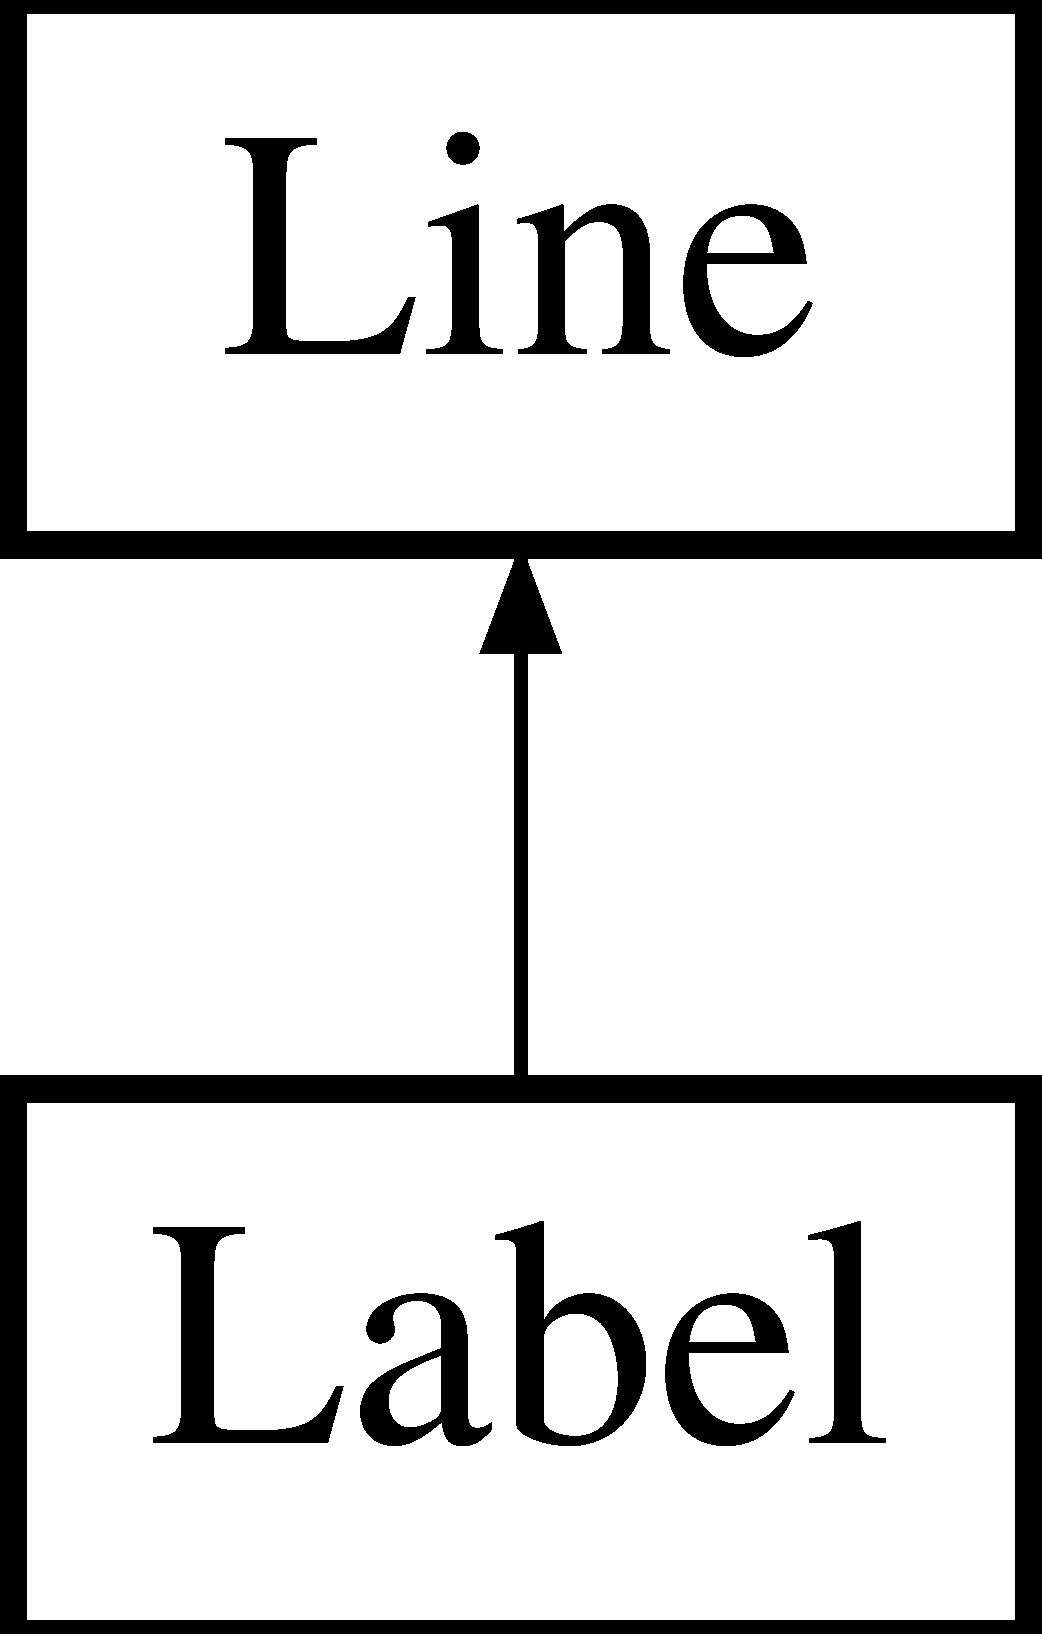
\includegraphics[height=2.000000cm]{class_label}
\end{center}
\end{figure}
\subsection*{Public Member Functions}
\begin{DoxyCompactItemize}
\item 
\mbox{\Hypertarget{class_label_a48e774efc0e6e5cd0bf63a94527add17}\label{class_label_a48e774efc0e6e5cd0bf63a94527add17}} 
\mbox{\hyperlink{class_label_a48e774efc0e6e5cd0bf63a94527add17}{Label}} (string)
\begin{DoxyCompactList}\small\item\em Constructor of the \mbox{\hyperlink{class_label}{Label}}. \end{DoxyCompactList}\item 
\mbox{\Hypertarget{class_label_ae0405d591a2ff63c03b104435e2a3066}\label{class_label_ae0405d591a2ff63c03b104435e2a3066}} 
virtual \mbox{\hyperlink{class_label_ae0405d591a2ff63c03b104435e2a3066}{$\sim$\+Label}} ()
\begin{DoxyCompactList}\small\item\em Destructor of the \mbox{\hyperlink{class_label}{Label}}. \end{DoxyCompactList}\item 
\mbox{\Hypertarget{class_label_afc727d8ae97b32660faf703b30edc77e}\label{class_label_afc727d8ae97b32660faf703b30edc77e}} 
virtual t\+\_\+\+Line \mbox{\hyperlink{class_label_afc727d8ae97b32660faf703b30edc77e}{type\+\_\+line}} ()
\begin{DoxyCompactList}\small\item\em get the type of the line \end{DoxyCompactList}\item 
\mbox{\Hypertarget{class_label_a6df2e96366cc459a6a8fa9642a6e69b6}\label{class_label_a6df2e96366cc459a6a8fa9642a6e69b6}} 
virtual string \mbox{\hyperlink{class_label_a6df2e96366cc459a6a8fa9642a6e69b6}{to\+\_\+string}} ()
\begin{DoxyCompactList}\small\item\em get the string of \mbox{\hyperlink{class_label}{Label}} \end{DoxyCompactList}\item 
\mbox{\Hypertarget{class_label_a8d48d53b6eb2c6024b7da507bfa5d00b}\label{class_label_a8d48d53b6eb2c6024b7da507bfa5d00b}} 
virtual string \mbox{\hyperlink{class_label_a8d48d53b6eb2c6024b7da507bfa5d00b}{get\+\_\+content}} ()
\begin{DoxyCompactList}\small\item\em get the string of the \mbox{\hyperlink{class_label}{Label}} \end{DoxyCompactList}\item 
\mbox{\Hypertarget{class_label_a16f1db5a51a093f3963a2d902bce845f}\label{class_label_a16f1db5a51a093f3963a2d902bce845f}} 
virtual void \mbox{\hyperlink{class_label_a16f1db5a51a093f3963a2d902bce845f}{set\+\_\+content}} (string)
\begin{DoxyCompactList}\small\item\em set the string of the \mbox{\hyperlink{class_label}{Label}} \end{DoxyCompactList}\item 
\mbox{\Hypertarget{class_label_af123355b73ac457171c3118052d145ac}\label{class_label_af123355b73ac457171c3118052d145ac}} 
virtual t\+\_\+\+Inst \mbox{\hyperlink{class_label_af123355b73ac457171c3118052d145ac}{get\+\_\+type}} ()
\begin{DoxyCompactList}\small\item\em return the type of the instruction \end{DoxyCompactList}\end{DoxyCompactItemize}
\subsection*{Additional Inherited Members}


\subsection{Detailed Description}
class representing an \mbox{\hyperlink{class_label}{Label}} herited by \mbox{\hyperlink{class_line}{Line}} 

The documentation for this class was generated from the following file\+:\begin{DoxyCompactItemize}
\item 
include/\mbox{\hyperlink{_label_8h}{Label.\+h}}\end{DoxyCompactItemize}

\hypertarget{class_line}{}\section{Line Class Reference}
\label{class_line}\index{Line@{Line}}


Abstract class representing an \mbox{\hyperlink{class_line}{Line}}.  




{\ttfamily \#include $<$Line.\+h$>$}

Inheritance diagram for Line\+:\begin{figure}[H]
\begin{center}
\leavevmode
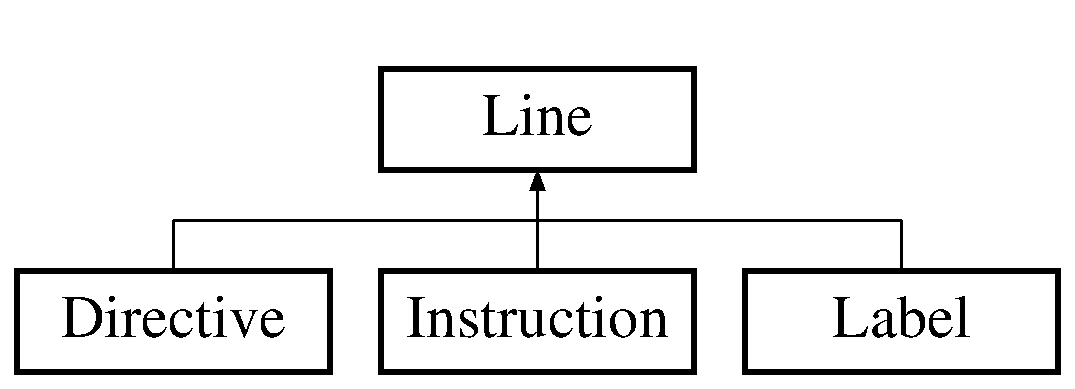
\includegraphics[height=2.000000cm]{class_line}
\end{center}
\end{figure}
\subsection*{Public Member Functions}
\begin{DoxyCompactItemize}
\item 
\mbox{\Hypertarget{class_line_a4a95bafcefa28672b3999deb011b9e50}\label{class_line_a4a95bafcefa28672b3999deb011b9e50}} 
virtual \mbox{\hyperlink{class_line_a4a95bafcefa28672b3999deb011b9e50}{$\sim$\+Line}} ()
\begin{DoxyCompactList}\small\item\em Virtual destructor. \end{DoxyCompactList}\item 
\mbox{\Hypertarget{class_line_aa7f74673c9c3a7423a513a5fb64bf825}\label{class_line_aa7f74673c9c3a7423a513a5fb64bf825}} 
virtual string \mbox{\hyperlink{class_line_aa7f74673c9c3a7423a513a5fb64bf825}{get\+\_\+content}} ()=0
\begin{DoxyCompactList}\small\item\em get the string of the line virtual getter \end{DoxyCompactList}\item 
\mbox{\Hypertarget{class_line_afa27867ffd08e6915d9e791d2ed0b448}\label{class_line_afa27867ffd08e6915d9e791d2ed0b448}} 
virtual void \mbox{\hyperlink{class_line_afa27867ffd08e6915d9e791d2ed0b448}{set\+\_\+content}} (string)=0
\begin{DoxyCompactList}\small\item\em set the string of the line virtual setter \end{DoxyCompactList}\item 
\mbox{\Hypertarget{class_line_a0cc2cdd9bc04649adebd1ff9b753bc85}\label{class_line_a0cc2cdd9bc04649adebd1ff9b753bc85}} 
virtual t\+\_\+\+Line \mbox{\hyperlink{class_line_a0cc2cdd9bc04649adebd1ff9b753bc85}{type\+\_\+line}} ()=0
\begin{DoxyCompactList}\small\item\em get the type of the line virtual accessor of the type \end{DoxyCompactList}\item 
virtual string \mbox{\hyperlink{class_line_a477523118f17d72f58f2912b391afc73}{to\+\_\+string}} ()=0
\begin{DoxyCompactList}\small\item\em get the name string accessor of the type line \end{DoxyCompactList}\item 
\mbox{\Hypertarget{class_line_a679ddcc8a7d6a634218f177b4d602bd5}\label{class_line_a679ddcc8a7d6a634218f177b4d602bd5}} 
virtual t\+\_\+\+Inst \mbox{\hyperlink{class_line_a679ddcc8a7d6a634218f177b4d602bd5}{get\+\_\+type}} ()=0
\begin{DoxyCompactList}\small\item\em return the type of the instruction \end{DoxyCompactList}\item 
\mbox{\Hypertarget{class_line_a57e724949fa0828dfdd2a1bb0f7db8d0}\label{class_line_a57e724949fa0828dfdd2a1bb0f7db8d0}} 
bool \mbox{\hyperlink{class_line_a57e724949fa0828dfdd2a1bb0f7db8d0}{is\+Inst}} ()
\begin{DoxyCompactList}\small\item\em tests if the line is an instruction \end{DoxyCompactList}\item 
\mbox{\Hypertarget{class_line_a8323f3df960924826199bd607198ac7f}\label{class_line_a8323f3df960924826199bd607198ac7f}} 
bool \mbox{\hyperlink{class_line_a8323f3df960924826199bd607198ac7f}{is\+Label}} ()
\begin{DoxyCompactList}\small\item\em tests if the line is a label \end{DoxyCompactList}\item 
\mbox{\Hypertarget{class_line_ad014e40a75c8a04e6a091ae4110579bc}\label{class_line_ad014e40a75c8a04e6a091ae4110579bc}} 
bool \mbox{\hyperlink{class_line_ad014e40a75c8a04e6a091ae4110579bc}{is\+Directive}} ()
\begin{DoxyCompactList}\small\item\em tests if the line is a directive \end{DoxyCompactList}\item 
\mbox{\Hypertarget{class_line_a66770cb09833f18ec4d5b494f5edae77}\label{class_line_a66770cb09833f18ec4d5b494f5edae77}} 
void \mbox{\hyperlink{class_line_a66770cb09833f18ec4d5b494f5edae77}{set\+\_\+next}} (\mbox{\hyperlink{class_line}{Line}} $\ast$newsuccessor)
\begin{DoxyCompactList}\small\item\em set the next line \end{DoxyCompactList}\item 
\mbox{\Hypertarget{class_line_ae834b48e9f1c9450f93ec7bb6a43fb1a}\label{class_line_ae834b48e9f1c9450f93ec7bb6a43fb1a}} 
\mbox{\hyperlink{class_line}{Line}} $\ast$ \mbox{\hyperlink{class_line_ae834b48e9f1c9450f93ec7bb6a43fb1a}{get\+\_\+prev}} ()
\begin{DoxyCompactList}\small\item\em get the previous line \end{DoxyCompactList}\item 
\mbox{\Hypertarget{class_line_abf7301d0514bf6dafdc9da9ad79a4341}\label{class_line_abf7301d0514bf6dafdc9da9ad79a4341}} 
void \mbox{\hyperlink{class_line_abf7301d0514bf6dafdc9da9ad79a4341}{set\+\_\+prev}} (\mbox{\hyperlink{class_line}{Line}} $\ast$newprev)
\begin{DoxyCompactList}\small\item\em set the previous line \end{DoxyCompactList}\item 
\mbox{\Hypertarget{class_line_a51b6d0f3c36a6aefb03be582277ca570}\label{class_line_a51b6d0f3c36a6aefb03be582277ca570}} 
\mbox{\hyperlink{class_line}{Line}} $\ast$ \mbox{\hyperlink{class_line_a51b6d0f3c36a6aefb03be582277ca570}{get\+\_\+next}} ()
\begin{DoxyCompactList}\small\item\em get the next line \end{DoxyCompactList}\item 
\mbox{\Hypertarget{class_line_a2f138ac1c387679c8569c4b5bf06a0f9}\label{class_line_a2f138ac1c387679c8569c4b5bf06a0f9}} 
void \mbox{\hyperlink{class_line_a2f138ac1c387679c8569c4b5bf06a0f9}{display}} ()
\begin{DoxyCompactList}\small\item\em display the content of the \mbox{\hyperlink{class_line}{Line}} \end{DoxyCompactList}\end{DoxyCompactItemize}
\subsection*{Protected Attributes}
\begin{DoxyCompactItemize}
\item 
\mbox{\Hypertarget{class_line_aa37e3e0b9ec8180ba796fcd970186437}\label{class_line_aa37e3e0b9ec8180ba796fcd970186437}} 
\mbox{\hyperlink{class_line}{Line}} $\ast$ {\bfseries \+\_\+next}
\item 
\mbox{\Hypertarget{class_line_a13163a448797ff8bc4f113202a6d4d4a}\label{class_line_a13163a448797ff8bc4f113202a6d4d4a}} 
\mbox{\hyperlink{class_line}{Line}} $\ast$ {\bfseries \+\_\+prev}
\item 
\mbox{\Hypertarget{class_line_a41059923f5c8e5a0f4f44d84bd8762aa}\label{class_line_a41059923f5c8e5a0f4f44d84bd8762aa}} 
string {\bfseries \+\_\+line}
\end{DoxyCompactItemize}


\subsection{Detailed Description}
Abstract class representing an \mbox{\hyperlink{class_line}{Line}}. 

\subsection{Member Function Documentation}
\mbox{\Hypertarget{class_line_a477523118f17d72f58f2912b391afc73}\label{class_line_a477523118f17d72f58f2912b391afc73}} 
\index{Line@{Line}!to\+\_\+string@{to\+\_\+string}}
\index{to\+\_\+string@{to\+\_\+string}!Line@{Line}}
\subsubsection{\texorpdfstring{to\+\_\+string()}{to\_string()}}
{\footnotesize\ttfamily virtual string Line\+::to\+\_\+string (\begin{DoxyParamCaption}{ }\end{DoxyParamCaption})\hspace{0.3cm}{\ttfamily [pure virtual]}}



get the name string accessor of the type line 



Implemented in \mbox{\hyperlink{class_instruction_aed87de5e9259f4f15dc885425528f1fe}{Instruction}}, \mbox{\hyperlink{class_directive_a2fd56d5580ad7a993782649d7867732f}{Directive}}, and \mbox{\hyperlink{class_label_a6df2e96366cc459a6a8fa9642a6e69b6}{Label}}.



The documentation for this class was generated from the following file\+:\begin{DoxyCompactItemize}
\item 
include/\mbox{\hyperlink{_line_8h}{Line.\+h}}\end{DoxyCompactItemize}

\hypertarget{class_loop}{}\section{Loop Class Reference}
\label{class_loop}\index{Loop@{Loop}}


class representing a \mbox{\hyperlink{class_loop}{Loop}} in a function  




{\ttfamily \#include $<$Loop.\+h$>$}

\subsection*{Public Member Functions}
\begin{DoxyCompactItemize}
\item 
\mbox{\Hypertarget{class_loop_a297fba15fcc47b206b5ffc204d1bd73c}\label{class_loop_a297fba15fcc47b206b5ffc204d1bd73c}} 
\mbox{\hyperlink{class_loop_a297fba15fcc47b206b5ffc204d1bd73c}{Loop}} (\mbox{\hyperlink{class_basic__block}{Basic\+\_\+block}} $\ast$, \mbox{\hyperlink{class_basic__block}{Basic\+\_\+block}} $\ast$)
\begin{DoxyCompactList}\small\item\em Constructor of a loop. \end{DoxyCompactList}\item 
\mbox{\Hypertarget{class_loop_ac25ba52a46e689c85e2720718615d767}\label{class_loop_ac25ba52a46e689c85e2720718615d767}} 
\mbox{\hyperlink{class_loop_ac25ba52a46e689c85e2720718615d767}{$\sim$\+Loop}} ()
\begin{DoxyCompactList}\small\item\em Destructor of a loop. \end{DoxyCompactList}\item 
\mbox{\Hypertarget{class_loop_a7c12f75026535ed0ed793d945cca5b26}\label{class_loop_a7c12f75026535ed0ed793d945cca5b26}} 
void \mbox{\hyperlink{class_loop_a7c12f75026535ed0ed793d945cca5b26}{set\+\_\+header}} (\mbox{\hyperlink{class_basic__block}{Basic\+\_\+block}} $\ast$)
\begin{DoxyCompactList}\small\item\em setter of the header of the loop \end{DoxyCompactList}\item 
\mbox{\Hypertarget{class_loop_ab5523a4e9881844ed445c18c809752cb}\label{class_loop_ab5523a4e9881844ed445c18c809752cb}} 
void \mbox{\hyperlink{class_loop_ab5523a4e9881844ed445c18c809752cb}{set\+\_\+latch}} (\mbox{\hyperlink{class_basic__block}{Basic\+\_\+block}} $\ast$)
\begin{DoxyCompactList}\small\item\em setter of the latch of the loop \end{DoxyCompactList}\item 
\mbox{\Hypertarget{class_loop_a3bd41bfb89e48a857327021a7584ea0e}\label{class_loop_a3bd41bfb89e48a857327021a7584ea0e}} 
\mbox{\hyperlink{class_basic__block}{Basic\+\_\+block}} $\ast$ \mbox{\hyperlink{class_loop_a3bd41bfb89e48a857327021a7584ea0e}{get\+\_\+header}} ()
\begin{DoxyCompactList}\small\item\em get the head of the loop \end{DoxyCompactList}\item 
\mbox{\Hypertarget{class_loop_ad8393fca8e80d2cb152f6ed9cbfa9ef9}\label{class_loop_ad8393fca8e80d2cb152f6ed9cbfa9ef9}} 
\mbox{\hyperlink{class_basic__block}{Basic\+\_\+block}} $\ast$ \mbox{\hyperlink{class_loop_ad8393fca8e80d2cb152f6ed9cbfa9ef9}{get\+\_\+latch}} ()
\begin{DoxyCompactList}\small\item\em get the latch of the loop \end{DoxyCompactList}\item 
\mbox{\Hypertarget{class_loop_a9c19796af1e978d32f80efc48035b061}\label{class_loop_a9c19796af1e978d32f80efc48035b061}} 
void \mbox{\hyperlink{class_loop_a9c19796af1e978d32f80efc48035b061}{display}} ()
\begin{DoxyCompactList}\small\item\em display the loop \end{DoxyCompactList}\item 
\mbox{\Hypertarget{class_loop_a333d1ba3bf5e448f7cd958c6d39beec2}\label{class_loop_a333d1ba3bf5e448f7cd958c6d39beec2}} 
int \mbox{\hyperlink{class_loop_a333d1ba3bf5e448f7cd958c6d39beec2}{nbr\+\_\+\+BB}} ()
\begin{DoxyCompactList}\small\item\em get the number of Basic block in the loop \end{DoxyCompactList}\item 
\mbox{\Hypertarget{class_loop_a5ec7079fa8bbce34a18b41b768d3a118}\label{class_loop_a5ec7079fa8bbce34a18b41b768d3a118}} 
void \mbox{\hyperlink{class_loop_a5ec7079fa8bbce34a18b41b768d3a118}{compute\+\_\+in\+\_\+loop\+\_\+\+BB}} ()
\begin{DoxyCompactList}\small\item\em compute the set of BB composing the loop \end{DoxyCompactList}\end{DoxyCompactItemize}


\subsection{Detailed Description}
class representing a \mbox{\hyperlink{class_loop}{Loop}} in a function 

The documentation for this class was generated from the following file\+:\begin{DoxyCompactItemize}
\item 
include/\mbox{\hyperlink{_loop_8h}{Loop.\+h}}\end{DoxyCompactItemize}

\hypertarget{class_node__dfg}{}\section{Node\+\_\+dfg Class Reference}
\label{class_node__dfg}\index{Node\+\_\+dfg@{Node\+\_\+dfg}}


class representing a node of data flow graph  




{\ttfamily \#include $<$Node\+\_\+dfg.\+h$>$}

\subsection*{Public Member Functions}
\begin{DoxyCompactItemize}
\item 
\mbox{\Hypertarget{class_node__dfg_ac9b79961aaadf29eecd03b227b4c0875}\label{class_node__dfg_ac9b79961aaadf29eecd03b227b4c0875}} 
\mbox{\hyperlink{class_node__dfg_ac9b79961aaadf29eecd03b227b4c0875}{Node\+\_\+dfg}} (\mbox{\hyperlink{class_instruction}{Instruction}} $\ast$)
\begin{DoxyCompactList}\small\item\em Constructor of \mbox{\hyperlink{class_node__dfg}{Node\+\_\+dfg}}. \end{DoxyCompactList}\item 
\mbox{\Hypertarget{class_node__dfg_a0a2a7c4634ad6802e7c69ab0d95957fa}\label{class_node__dfg_a0a2a7c4634ad6802e7c69ab0d95957fa}} 
\mbox{\hyperlink{class_node__dfg_a0a2a7c4634ad6802e7c69ab0d95957fa}{$\sim$\+Node\+\_\+dfg}} ()
\begin{DoxyCompactList}\small\item\em Destructor of \mbox{\hyperlink{class_node__dfg}{Node\+\_\+dfg}}. \end{DoxyCompactList}\item 
\mbox{\Hypertarget{class_node__dfg_adc4a8e37604e57eec03fecaaca094fb5}\label{class_node__dfg_adc4a8e37604e57eec03fecaaca094fb5}} 
\mbox{\hyperlink{struct_arc__t}{Arc\+\_\+t}} $\ast$ \mbox{\hyperlink{class_node__dfg_adc4a8e37604e57eec03fecaaca094fb5}{get\+\_\+arc}} (int i)
\begin{DoxyCompactList}\small\item\em get the ith arc of the arc list \end{DoxyCompactList}\item 
\mbox{\Hypertarget{class_node__dfg_a27b393ab78abb865ef7c4e494de894da}\label{class_node__dfg_a27b393ab78abb865ef7c4e494de894da}} 
void {\bfseries remove\+\_\+arc} (int index)
\item 
\mbox{\Hypertarget{class_node__dfg_a0f65316cde0b35e7755d4ebf009b009b}\label{class_node__dfg_a0f65316cde0b35e7755d4ebf009b009b}} 
void {\bfseries remove\+\_\+pred} (int index)
\item 
\mbox{\Hypertarget{class_node__dfg_a6ebd568efb70f729f6e355cdd46a5185}\label{class_node__dfg_a6ebd568efb70f729f6e355cdd46a5185}} 
list$<$ \mbox{\hyperlink{struct_arc__t}{Arc\+\_\+t}} $\ast$ $>$\+::iterator {\bfseries arcs\+\_\+begin} ()
\item 
\mbox{\Hypertarget{class_node__dfg_a5a49217bcb16aaf7e94e4e156d9a9d53}\label{class_node__dfg_a5a49217bcb16aaf7e94e4e156d9a9d53}} 
list$<$ \mbox{\hyperlink{struct_arc__t}{Arc\+\_\+t}} $\ast$ $>$\+::iterator {\bfseries arcs\+\_\+end} ()
\item 
\mbox{\Hypertarget{class_node__dfg_a85d42a5cc1d6feacf403a8569a813074}\label{class_node__dfg_a85d42a5cc1d6feacf403a8569a813074}} 
int \mbox{\hyperlink{class_node__dfg_a85d42a5cc1d6feacf403a8569a813074}{get\+\_\+nb\+\_\+arcs}} ()
\begin{DoxyCompactList}\small\item\em get the number of arcs \end{DoxyCompactList}\item 
\mbox{\Hypertarget{class_node__dfg_a8f20c21a0ffb2e224cc426148362c249}\label{class_node__dfg_a8f20c21a0ffb2e224cc426148362c249}} 
\mbox{\hyperlink{class_instruction}{Instruction}} $\ast$ \mbox{\hyperlink{class_node__dfg_a8f20c21a0ffb2e224cc426148362c249}{get\+\_\+instruction}} ()
\begin{DoxyCompactList}\small\item\em get the \mbox{\hyperlink{class_instruction}{Instruction}} \end{DoxyCompactList}\item 
\mbox{\Hypertarget{class_node__dfg_add9d669804bc8ad4a4b806221d9ef9e9}\label{class_node__dfg_add9d669804bc8ad4a4b806221d9ef9e9}} 
void \mbox{\hyperlink{class_node__dfg_add9d669804bc8ad4a4b806221d9ef9e9}{add\+\_\+successeur}} (\mbox{\hyperlink{struct_arc__t}{Arc\+\_\+t}} $\ast$)
\begin{DoxyCompactList}\small\item\em add an arc to the arc list \end{DoxyCompactList}\item 
\mbox{\Hypertarget{class_node__dfg_a8cc89b32dbe15bcf399725955a643551}\label{class_node__dfg_a8cc89b32dbe15bcf399725955a643551}} 
void \mbox{\hyperlink{class_node__dfg_a8cc89b32dbe15bcf399725955a643551}{add\+\_\+predecesseur}} (\mbox{\hyperlink{class_node__dfg}{Node\+\_\+dfg}} $\ast$)
\begin{DoxyCompactList}\small\item\em add a predecessor to the predecessor list \end{DoxyCompactList}\item 
\mbox{\Hypertarget{class_node__dfg_adef5e6e3362133f6adb38d404c8d8cf6}\label{class_node__dfg_adef5e6e3362133f6adb38d404c8d8cf6}} 
int \mbox{\hyperlink{class_node__dfg_adef5e6e3362133f6adb38d404c8d8cf6}{nb\+\_\+preds}} ()
\begin{DoxyCompactList}\small\item\em get the number of predecessors \end{DoxyCompactList}\item 
\mbox{\Hypertarget{class_node__dfg_a769af0d7836679d6ee9abcc55d399887}\label{class_node__dfg_a769af0d7836679d6ee9abcc55d399887}} 
list$<$ \mbox{\hyperlink{class_node__dfg}{Node\+\_\+dfg}} $\ast$ $>$\+::iterator {\bfseries pred\+\_\+begin} ()
\item 
\mbox{\Hypertarget{class_node__dfg_a86fc141e0697ae944900625212579957}\label{class_node__dfg_a86fc141e0697ae944900625212579957}} 
list$<$ \mbox{\hyperlink{class_node__dfg}{Node\+\_\+dfg}} $\ast$ $>$\+::iterator {\bfseries pred\+\_\+end} ()
\item 
\mbox{\Hypertarget{class_node__dfg_a83747917d9c87b11633779731bcda162}\label{class_node__dfg_a83747917d9c87b11633779731bcda162}} 
void \mbox{\hyperlink{class_node__dfg_a83747917d9c87b11633779731bcda162}{set\+\_\+instruction}} (\mbox{\hyperlink{class_instruction}{Instruction}} $\ast$)
\begin{DoxyCompactList}\small\item\em set the \mbox{\hyperlink{class_instruction}{Instruction}} \end{DoxyCompactList}\item 
\mbox{\Hypertarget{class_node__dfg_a395b778a0b23ae2bcfd6081d84661239}\label{class_node__dfg_a395b778a0b23ae2bcfd6081d84661239}} 
int {\bfseries compute\+\_\+weight} ()
\item 
\mbox{\Hypertarget{class_node__dfg_af23f48b1521a90178cc5c9a59da3ab3c}\label{class_node__dfg_af23f48b1521a90178cc5c9a59da3ab3c}} 
void \mbox{\hyperlink{class_node__dfg_af23f48b1521a90178cc5c9a59da3ab3c}{set\+\_\+weight}} (int)
\begin{DoxyCompactList}\small\item\em set the weight \end{DoxyCompactList}\item 
\mbox{\Hypertarget{class_node__dfg_a561e80f51cb9a71b22f22e8d2e6685de}\label{class_node__dfg_a561e80f51cb9a71b22f22e8d2e6685de}} 
int \mbox{\hyperlink{class_node__dfg_a561e80f51cb9a71b22f22e8d2e6685de}{get\+\_\+weight}} ()
\begin{DoxyCompactList}\small\item\em get the weight \end{DoxyCompactList}\item 
\mbox{\Hypertarget{class_node__dfg_a613aa3ee9ce2eb99df07258cbdd5293f}\label{class_node__dfg_a613aa3ee9ce2eb99df07258cbdd5293f}} 
int {\bfseries compute\+\_\+nb\+\_\+descendant} (int nb\+\_\+instr, int $\ast$deja\+\_\+comptes)
\item 
\mbox{\Hypertarget{class_node__dfg_a9aa775f727e6c542cd714894219046f3}\label{class_node__dfg_a9aa775f727e6c542cd714894219046f3}} 
void \mbox{\hyperlink{class_node__dfg_a9aa775f727e6c542cd714894219046f3}{set\+\_\+nb\+\_\+descendant}} (int)
\begin{DoxyCompactList}\small\item\em set the number of descendant \end{DoxyCompactList}\item 
\mbox{\Hypertarget{class_node__dfg_a9baa0a6be056b7d1ee290c404f2216f5}\label{class_node__dfg_a9baa0a6be056b7d1ee290c404f2216f5}} 
int \mbox{\hyperlink{class_node__dfg_a9baa0a6be056b7d1ee290c404f2216f5}{get\+\_\+nb\+\_\+descendant}} ()
\begin{DoxyCompactList}\small\item\em get the number of descendant \end{DoxyCompactList}\item 
\mbox{\Hypertarget{class_node__dfg_ad9fe88cf90fa2282806edbc64f51331e}\label{class_node__dfg_ad9fe88cf90fa2282806edbc64f51331e}} 
void {\bfseries set\+\_\+tready} (int t)
\item 
\mbox{\Hypertarget{class_node__dfg_a05e8db316dd2db8b0946167763585c7b}\label{class_node__dfg_a05e8db316dd2db8b0946167763585c7b}} 
int {\bfseries get\+\_\+tready} ()
\end{DoxyCompactItemize}


\subsection{Detailed Description}
class representing a node of data flow graph 

The documentation for this class was generated from the following file\+:\begin{DoxyCompactItemize}
\item 
include/\mbox{\hyperlink{_node__dfg_8h}{Node\+\_\+dfg.\+h}}\end{DoxyCompactItemize}

\hypertarget{class_operand}{}\section{Operand Class Reference}
\label{class_operand}\index{Operand@{Operand}}


Abstract class representing an operand.  




{\ttfamily \#include $<$Operand.\+h$>$}

Inheritance diagram for Operand\+:\begin{figure}[H]
\begin{center}
\leavevmode
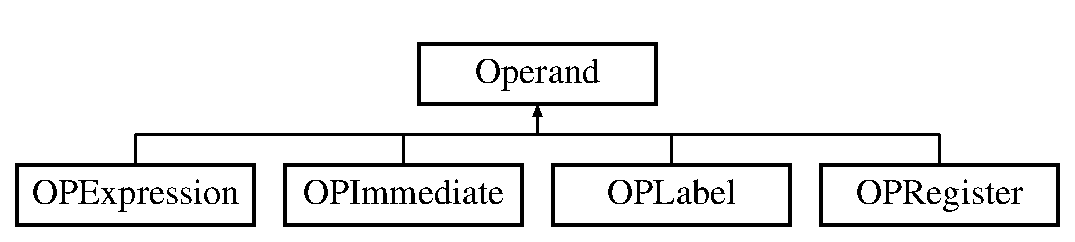
\includegraphics[height=2.000000cm]{class_operand}
\end{center}
\end{figure}
\subsection*{Public Member Functions}
\begin{DoxyCompactItemize}
\item 
\mbox{\Hypertarget{class_operand_aa6ef1ffa183381edb413f9b93782a67b}\label{class_operand_aa6ef1ffa183381edb413f9b93782a67b}} 
virtual \mbox{\hyperlink{class_operand_aa6ef1ffa183381edb413f9b93782a67b}{$\sim$\+Operand}} ()
\begin{DoxyCompactList}\small\item\em Virtual destructor. \end{DoxyCompactList}\item 
\mbox{\Hypertarget{class_operand_a2bf3ad8b34d39cb35ff743ffcc0f4675}\label{class_operand_a2bf3ad8b34d39cb35ff743ffcc0f4675}} 
virtual string \mbox{\hyperlink{class_operand_a2bf3ad8b34d39cb35ff743ffcc0f4675}{get\+\_\+op}} ()=0
\begin{DoxyCompactList}\small\item\em Get the operand value virtual accessor of the operand. \end{DoxyCompactList}\item 
\mbox{\Hypertarget{class_operand_a0895c39d7b97ea56f074d242e8232c78}\label{class_operand_a0895c39d7b97ea56f074d242e8232c78}} 
virtual void \mbox{\hyperlink{class_operand_a0895c39d7b97ea56f074d242e8232c78}{set\+\_\+op}} (string)=0
\begin{DoxyCompactList}\small\item\em set the operand value virtual setter of the operand \end{DoxyCompactList}\item 
virtual t\+\_\+\+Op\+Type \mbox{\hyperlink{class_operand_afd469e305a467e2574f34ac9bd6c62b0}{get\+\_\+op\+\_\+type}} ()=0
\begin{DoxyCompactList}\small\item\em get the operator type virtual accessor of accessor \end{DoxyCompactList}\item 
virtual string \mbox{\hyperlink{class_operand_a28aed96d5fafee66be81c30c1435ad00}{to\+\_\+string}} ()=0
\begin{DoxyCompactList}\small\item\em virtual tostring \end{DoxyCompactList}\item 
\mbox{\Hypertarget{class_operand_a12ccf172b496bc2fee04f732d144641b}\label{class_operand_a12ccf172b496bc2fee04f732d144641b}} 
bool {\bfseries is\+O\+P\+Label} ()
\item 
\mbox{\Hypertarget{class_operand_a5c596cb4bdb24227118697d33d9833eb}\label{class_operand_a5c596cb4bdb24227118697d33d9833eb}} 
bool {\bfseries is\+O\+P\+Register} ()
\item 
\mbox{\Hypertarget{class_operand_a91f072d08b59eaa343e512e644c8efb4}\label{class_operand_a91f072d08b59eaa343e512e644c8efb4}} 
bool {\bfseries is\+O\+P\+Immediate} ()
\end{DoxyCompactItemize}
\subsection*{Protected Attributes}
\begin{DoxyCompactItemize}
\item 
\mbox{\Hypertarget{class_operand_af70a183445064a0106d41dfeea681790}\label{class_operand_af70a183445064a0106d41dfeea681790}} 
string {\bfseries \+\_\+oper}
\end{DoxyCompactItemize}


\subsection{Detailed Description}
Abstract class representing an operand. 

\subsection{Member Function Documentation}
\mbox{\Hypertarget{class_operand_afd469e305a467e2574f34ac9bd6c62b0}\label{class_operand_afd469e305a467e2574f34ac9bd6c62b0}} 
\index{Operand@{Operand}!get\+\_\+op\+\_\+type@{get\+\_\+op\+\_\+type}}
\index{get\+\_\+op\+\_\+type@{get\+\_\+op\+\_\+type}!Operand@{Operand}}
\subsubsection{\texorpdfstring{get\+\_\+op\+\_\+type()}{get\_op\_type()}}
{\footnotesize\ttfamily virtual t\+\_\+\+Op\+Type Operand\+::get\+\_\+op\+\_\+type (\begin{DoxyParamCaption}{ }\end{DoxyParamCaption})\hspace{0.3cm}{\ttfamily [pure virtual]}}



get the operator type virtual accessor of accessor 

\begin{DoxyReturn}{Returns}
return the \mbox{\hyperlink{class_operand}{Operand}} type as enum 
\end{DoxyReturn}


Implemented in \mbox{\hyperlink{class_o_p_register_a1be03d6e6422510a1fd12d1f13dfd601}{O\+P\+Register}}, \mbox{\hyperlink{class_o_p_immediate_aed01353798ae57936a9f77dd05eafa88}{O\+P\+Immediate}}, \mbox{\hyperlink{class_o_p_label_a1a6ec701c549a6475d44ffcced1c23b5}{O\+P\+Label}}, and \mbox{\hyperlink{class_o_p_expression_a06f8902130516437d5d93c43a5efcbd2}{O\+P\+Expression}}.

\mbox{\Hypertarget{class_operand_a28aed96d5fafee66be81c30c1435ad00}\label{class_operand_a28aed96d5fafee66be81c30c1435ad00}} 
\index{Operand@{Operand}!to\+\_\+string@{to\+\_\+string}}
\index{to\+\_\+string@{to\+\_\+string}!Operand@{Operand}}
\subsubsection{\texorpdfstring{to\+\_\+string()}{to\_string()}}
{\footnotesize\ttfamily virtual string Operand\+::to\+\_\+string (\begin{DoxyParamCaption}{ }\end{DoxyParamCaption})\hspace{0.3cm}{\ttfamily [pure virtual]}}



virtual tostring 

\begin{DoxyReturn}{Returns}
return the Object as string 
\end{DoxyReturn}


Implemented in \mbox{\hyperlink{class_o_p_register_a9f55bdff75224fb18973a9e913a4022f}{O\+P\+Register}}, \mbox{\hyperlink{class_o_p_immediate_a12bc613de3bff73ead8632dafd8050a0}{O\+P\+Immediate}}, \mbox{\hyperlink{class_o_p_label_a51c4e8f45422f03edcb71d472cf5e973}{O\+P\+Label}}, and \mbox{\hyperlink{class_o_p_expression_a0a6ee03eb083791028eeae021f4ff47b}{O\+P\+Expression}}.



The documentation for this class was generated from the following file\+:\begin{DoxyCompactItemize}
\item 
include/\mbox{\hyperlink{_operand_8h}{Operand.\+h}}\end{DoxyCompactItemize}

\hypertarget{class_o_p_expression}{}\section{O\+P\+Expression Class Reference}
\label{class_o_p_expression}\index{O\+P\+Expression@{O\+P\+Expression}}


class representing an expression herited by \mbox{\hyperlink{class_operand}{Operand}}  




{\ttfamily \#include $<$O\+P\+Expression.\+h$>$}

Inheritance diagram for O\+P\+Expression\+:\begin{figure}[H]
\begin{center}
\leavevmode
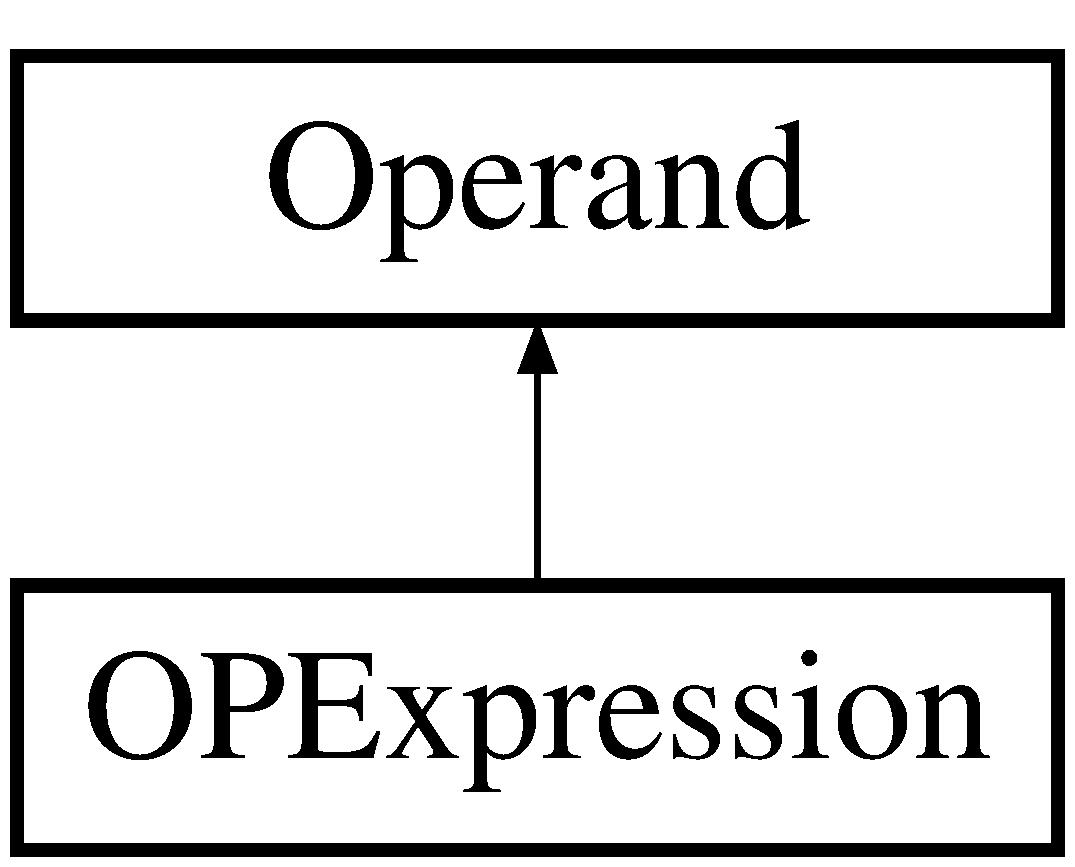
\includegraphics[height=2.000000cm]{class_o_p_expression}
\end{center}
\end{figure}
\subsection*{Public Member Functions}
\begin{DoxyCompactItemize}
\item 
\mbox{\Hypertarget{class_o_p_expression_a5784034daef8568869fe0bb5ecfbcdcf}\label{class_o_p_expression_a5784034daef8568869fe0bb5ecfbcdcf}} 
\mbox{\hyperlink{class_o_p_expression_a5784034daef8568869fe0bb5ecfbcdcf}{O\+P\+Expression}} (string)
\begin{DoxyCompactList}\small\item\em Constructor of the Expression class. \end{DoxyCompactList}\item 
\mbox{\Hypertarget{class_o_p_expression_a5ea892d89208ccb593510ee63ef42a19}\label{class_o_p_expression_a5ea892d89208ccb593510ee63ef42a19}} 
virtual \mbox{\hyperlink{class_o_p_expression_a5ea892d89208ccb593510ee63ef42a19}{$\sim$\+O\+P\+Expression}} ()
\begin{DoxyCompactList}\small\item\em Destructor of the Expression class. \end{DoxyCompactList}\item 
virtual string \mbox{\hyperlink{class_o_p_expression_acf86deca614626b803bc3c29facbefef}{get\+\_\+op}} ()
\begin{DoxyCompactList}\small\item\em Get the operand value. \end{DoxyCompactList}\item 
virtual t\+\_\+\+Op\+Type \mbox{\hyperlink{class_o_p_expression_a06f8902130516437d5d93c43a5efcbd2}{get\+\_\+op\+\_\+type}} ()
\begin{DoxyCompactList}\small\item\em get the operator type \end{DoxyCompactList}\item 
virtual string \mbox{\hyperlink{class_o_p_expression_a0a6ee03eb083791028eeae021f4ff47b}{to\+\_\+string}} ()
\begin{DoxyCompactList}\small\item\em tostring \end{DoxyCompactList}\item 
\mbox{\Hypertarget{class_o_p_expression_a3cfeacf4f76611d374be3caa9de80a05}\label{class_o_p_expression_a3cfeacf4f76611d374be3caa9de80a05}} 
virtual void \mbox{\hyperlink{class_o_p_expression_a3cfeacf4f76611d374be3caa9de80a05}{set\+\_\+op}} (string)
\begin{DoxyCompactList}\small\item\em set the operand value setter of the operand \end{DoxyCompactList}\end{DoxyCompactItemize}
\subsection*{Additional Inherited Members}


\subsection{Detailed Description}
class representing an expression herited by \mbox{\hyperlink{class_operand}{Operand}} 

\subsection{Member Function Documentation}
\mbox{\Hypertarget{class_o_p_expression_acf86deca614626b803bc3c29facbefef}\label{class_o_p_expression_acf86deca614626b803bc3c29facbefef}} 
\index{O\+P\+Expression@{O\+P\+Expression}!get\+\_\+op@{get\+\_\+op}}
\index{get\+\_\+op@{get\+\_\+op}!O\+P\+Expression@{O\+P\+Expression}}
\subsubsection{\texorpdfstring{get\+\_\+op()}{get\_op()}}
{\footnotesize\ttfamily virtual string O\+P\+Expression\+::get\+\_\+op (\begin{DoxyParamCaption}{ }\end{DoxyParamCaption})\hspace{0.3cm}{\ttfamily [virtual]}}



Get the operand value. 

\begin{DoxyReturn}{Returns}
return the string of the Expression 
\end{DoxyReturn}


Implements \mbox{\hyperlink{class_operand_a2bf3ad8b34d39cb35ff743ffcc0f4675}{Operand}}.

\mbox{\Hypertarget{class_o_p_expression_a06f8902130516437d5d93c43a5efcbd2}\label{class_o_p_expression_a06f8902130516437d5d93c43a5efcbd2}} 
\index{O\+P\+Expression@{O\+P\+Expression}!get\+\_\+op\+\_\+type@{get\+\_\+op\+\_\+type}}
\index{get\+\_\+op\+\_\+type@{get\+\_\+op\+\_\+type}!O\+P\+Expression@{O\+P\+Expression}}
\subsubsection{\texorpdfstring{get\+\_\+op\+\_\+type()}{get\_op\_type()}}
{\footnotesize\ttfamily virtual t\+\_\+\+Op\+Type O\+P\+Expression\+::get\+\_\+op\+\_\+type (\begin{DoxyParamCaption}{ }\end{DoxyParamCaption})\hspace{0.3cm}{\ttfamily [virtual]}}



get the operator type 

\begin{DoxyReturn}{Returns}
return the \mbox{\hyperlink{class_operand}{Operand}} type as enum 
\end{DoxyReturn}


Implements \mbox{\hyperlink{class_operand_afd469e305a467e2574f34ac9bd6c62b0}{Operand}}.

\mbox{\Hypertarget{class_o_p_expression_a0a6ee03eb083791028eeae021f4ff47b}\label{class_o_p_expression_a0a6ee03eb083791028eeae021f4ff47b}} 
\index{O\+P\+Expression@{O\+P\+Expression}!to\+\_\+string@{to\+\_\+string}}
\index{to\+\_\+string@{to\+\_\+string}!O\+P\+Expression@{O\+P\+Expression}}
\subsubsection{\texorpdfstring{to\+\_\+string()}{to\_string()}}
{\footnotesize\ttfamily virtual string O\+P\+Expression\+::to\+\_\+string (\begin{DoxyParamCaption}{ }\end{DoxyParamCaption})\hspace{0.3cm}{\ttfamily [virtual]}}



tostring 

\begin{DoxyReturn}{Returns}
return the Object as string 
\end{DoxyReturn}


Implements \mbox{\hyperlink{class_operand_a28aed96d5fafee66be81c30c1435ad00}{Operand}}.



The documentation for this class was generated from the following file\+:\begin{DoxyCompactItemize}
\item 
include/\mbox{\hyperlink{_o_p_expression_8h}{O\+P\+Expression.\+h}}\end{DoxyCompactItemize}

\hypertarget{class_o_p_immediate}{}\section{O\+P\+Immediate Class Reference}
\label{class_o_p_immediate}\index{O\+P\+Immediate@{O\+P\+Immediate}}


class representing an Immediate herited by \mbox{\hyperlink{class_operand}{Operand}}  




{\ttfamily \#include $<$O\+P\+Immediate.\+h$>$}

Inheritance diagram for O\+P\+Immediate\+:\begin{figure}[H]
\begin{center}
\leavevmode
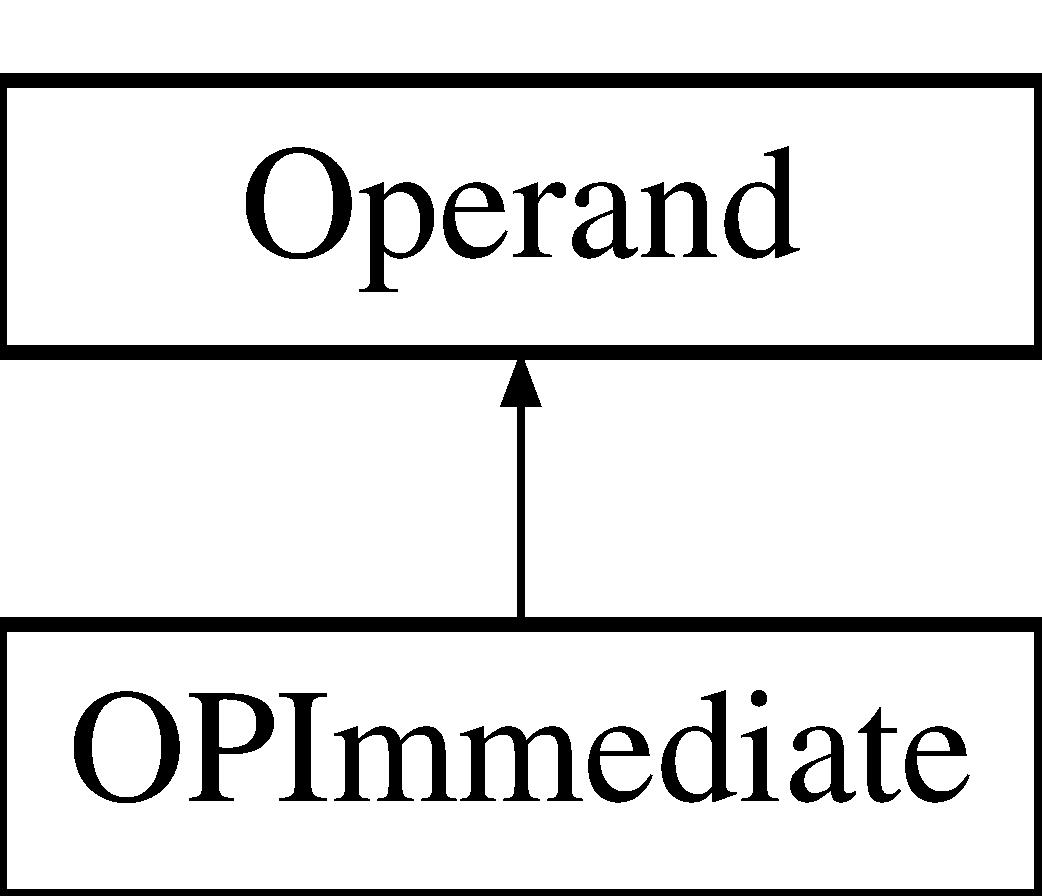
\includegraphics[height=2.000000cm]{class_o_p_immediate}
\end{center}
\end{figure}
\subsection*{Public Member Functions}
\begin{DoxyCompactItemize}
\item 
\mbox{\Hypertarget{class_o_p_immediate_ab047dac5f3390947a21e4ab118c05857}\label{class_o_p_immediate_ab047dac5f3390947a21e4ab118c05857}} 
\mbox{\hyperlink{class_o_p_immediate_ab047dac5f3390947a21e4ab118c05857}{O\+P\+Immediate}} (string)
\begin{DoxyCompactList}\small\item\em Constructor of the Immediate Class. \end{DoxyCompactList}\item 
\mbox{\Hypertarget{class_o_p_immediate_ae940dcf9e9050227a94c759a0cae6861}\label{class_o_p_immediate_ae940dcf9e9050227a94c759a0cae6861}} 
\mbox{\hyperlink{class_o_p_immediate_ae940dcf9e9050227a94c759a0cae6861}{O\+P\+Immediate}} (int)
\begin{DoxyCompactList}\small\item\em Constructor of the Immediate Class. \end{DoxyCompactList}\item 
\mbox{\Hypertarget{class_o_p_immediate_af7f51ae61e075e02817d6ecd7441408f}\label{class_o_p_immediate_af7f51ae61e075e02817d6ecd7441408f}} 
virtual \mbox{\hyperlink{class_o_p_immediate_af7f51ae61e075e02817d6ecd7441408f}{$\sim$\+O\+P\+Immediate}} ()
\begin{DoxyCompactList}\small\item\em Destructor of the Immediate Class. \end{DoxyCompactList}\item 
virtual string \mbox{\hyperlink{class_o_p_immediate_ad714fb614c0d8f4afa1157a34b2936fd}{get\+\_\+op}} ()
\begin{DoxyCompactList}\small\item\em Get the string of the operand. \end{DoxyCompactList}\item 
virtual t\+\_\+\+Op\+Type \mbox{\hyperlink{class_o_p_immediate_aed01353798ae57936a9f77dd05eafa88}{get\+\_\+op\+\_\+type}} ()
\begin{DoxyCompactList}\small\item\em get the operator type \end{DoxyCompactList}\item 
virtual string \mbox{\hyperlink{class_o_p_immediate_a12bc613de3bff73ead8632dafd8050a0}{to\+\_\+string}} ()
\begin{DoxyCompactList}\small\item\em tostring \end{DoxyCompactList}\item 
\mbox{\Hypertarget{class_o_p_immediate_ae5d6c30c6bff17de4e7fabb24cf6bf59}\label{class_o_p_immediate_ae5d6c30c6bff17de4e7fabb24cf6bf59}} 
virtual void \mbox{\hyperlink{class_o_p_immediate_ae5d6c30c6bff17de4e7fabb24cf6bf59}{set\+\_\+op}} (string)
\begin{DoxyCompactList}\small\item\em set the string of the operand setter of the operand \end{DoxyCompactList}\end{DoxyCompactItemize}
\subsection*{Additional Inherited Members}


\subsection{Detailed Description}
class representing an Immediate herited by \mbox{\hyperlink{class_operand}{Operand}} 

\subsection{Member Function Documentation}
\mbox{\Hypertarget{class_o_p_immediate_ad714fb614c0d8f4afa1157a34b2936fd}\label{class_o_p_immediate_ad714fb614c0d8f4afa1157a34b2936fd}} 
\index{O\+P\+Immediate@{O\+P\+Immediate}!get\+\_\+op@{get\+\_\+op}}
\index{get\+\_\+op@{get\+\_\+op}!O\+P\+Immediate@{O\+P\+Immediate}}
\subsubsection{\texorpdfstring{get\+\_\+op()}{get\_op()}}
{\footnotesize\ttfamily virtual string O\+P\+Immediate\+::get\+\_\+op (\begin{DoxyParamCaption}{ }\end{DoxyParamCaption})\hspace{0.3cm}{\ttfamily [virtual]}}



Get the string of the operand. 

\begin{DoxyReturn}{Returns}
return the string of the Immediate 
\end{DoxyReturn}


Implements \mbox{\hyperlink{class_operand_a2bf3ad8b34d39cb35ff743ffcc0f4675}{Operand}}.

\mbox{\Hypertarget{class_o_p_immediate_aed01353798ae57936a9f77dd05eafa88}\label{class_o_p_immediate_aed01353798ae57936a9f77dd05eafa88}} 
\index{O\+P\+Immediate@{O\+P\+Immediate}!get\+\_\+op\+\_\+type@{get\+\_\+op\+\_\+type}}
\index{get\+\_\+op\+\_\+type@{get\+\_\+op\+\_\+type}!O\+P\+Immediate@{O\+P\+Immediate}}
\subsubsection{\texorpdfstring{get\+\_\+op\+\_\+type()}{get\_op\_type()}}
{\footnotesize\ttfamily virtual t\+\_\+\+Op\+Type O\+P\+Immediate\+::get\+\_\+op\+\_\+type (\begin{DoxyParamCaption}{ }\end{DoxyParamCaption})\hspace{0.3cm}{\ttfamily [virtual]}}



get the operator type 

\begin{DoxyReturn}{Returns}
return the \mbox{\hyperlink{class_operand}{Operand}} type as enum 
\end{DoxyReturn}


Implements \mbox{\hyperlink{class_operand_afd469e305a467e2574f34ac9bd6c62b0}{Operand}}.

\mbox{\Hypertarget{class_o_p_immediate_a12bc613de3bff73ead8632dafd8050a0}\label{class_o_p_immediate_a12bc613de3bff73ead8632dafd8050a0}} 
\index{O\+P\+Immediate@{O\+P\+Immediate}!to\+\_\+string@{to\+\_\+string}}
\index{to\+\_\+string@{to\+\_\+string}!O\+P\+Immediate@{O\+P\+Immediate}}
\subsubsection{\texorpdfstring{to\+\_\+string()}{to\_string()}}
{\footnotesize\ttfamily virtual string O\+P\+Immediate\+::to\+\_\+string (\begin{DoxyParamCaption}{ }\end{DoxyParamCaption})\hspace{0.3cm}{\ttfamily [virtual]}}



tostring 

\begin{DoxyReturn}{Returns}
return the name of the Object as string 
\end{DoxyReturn}


Implements \mbox{\hyperlink{class_operand_a28aed96d5fafee66be81c30c1435ad00}{Operand}}.



The documentation for this class was generated from the following file\+:\begin{DoxyCompactItemize}
\item 
include/\mbox{\hyperlink{_o_p_immediate_8h}{O\+P\+Immediate.\+h}}\end{DoxyCompactItemize}

\hypertarget{class_o_p_label}{}\section{O\+P\+Label Class Reference}
\label{class_o_p_label}\index{O\+P\+Label@{O\+P\+Label}}


class representing a \mbox{\hyperlink{class_label}{Label}} herited by \mbox{\hyperlink{class_operand}{Operand}}  




{\ttfamily \#include $<$O\+P\+Label.\+h$>$}

Inheritance diagram for O\+P\+Label\+:\begin{figure}[H]
\begin{center}
\leavevmode
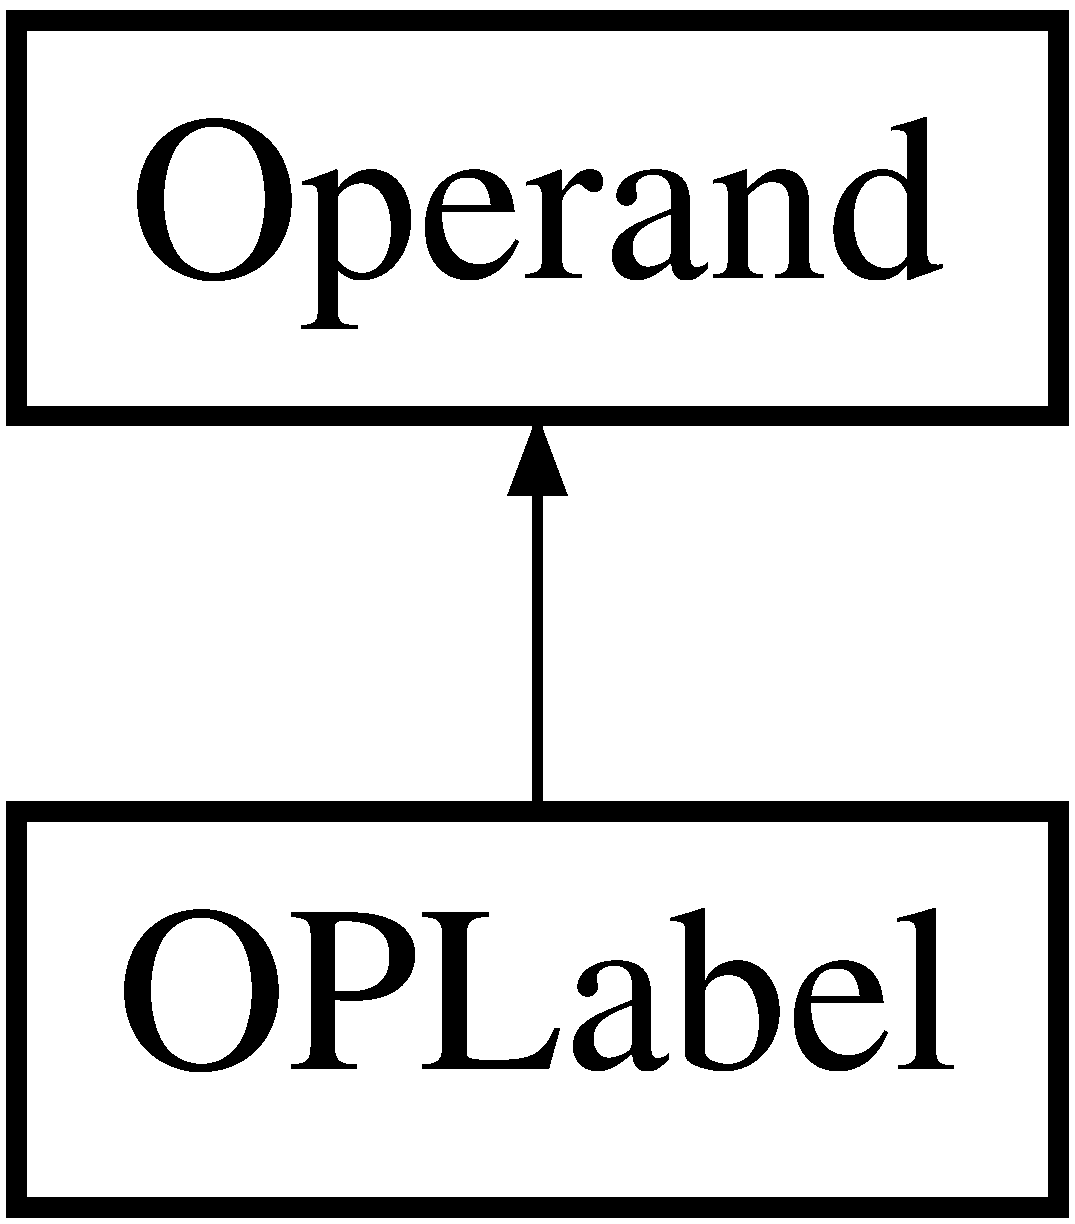
\includegraphics[height=2.000000cm]{class_o_p_label}
\end{center}
\end{figure}
\subsection*{Public Member Functions}
\begin{DoxyCompactItemize}
\item 
\mbox{\Hypertarget{class_o_p_label_a5405b78894658047362a328e750f88b4}\label{class_o_p_label_a5405b78894658047362a328e750f88b4}} 
\mbox{\hyperlink{class_o_p_label_a5405b78894658047362a328e750f88b4}{O\+P\+Label}} (string)
\begin{DoxyCompactList}\small\item\em Constructor of the \mbox{\hyperlink{class_label}{Label}} Class. \end{DoxyCompactList}\item 
\mbox{\Hypertarget{class_o_p_label_ab25553d41606e880a622e09d5c09129d}\label{class_o_p_label_ab25553d41606e880a622e09d5c09129d}} 
virtual \mbox{\hyperlink{class_o_p_label_ab25553d41606e880a622e09d5c09129d}{$\sim$\+O\+P\+Label}} ()
\begin{DoxyCompactList}\small\item\em Destructor of the \mbox{\hyperlink{class_label}{Label}} Class. \end{DoxyCompactList}\item 
\mbox{\Hypertarget{class_o_p_label_a1c933d10a7b2267bae3bea6c385d466f}\label{class_o_p_label_a1c933d10a7b2267bae3bea6c385d466f}} 
virtual string \mbox{\hyperlink{class_o_p_label_a1c933d10a7b2267bae3bea6c385d466f}{get\+\_\+op}} ()
\begin{DoxyCompactList}\small\item\em Get the string of the operand accessor of the operand. \end{DoxyCompactList}\item 
virtual t\+\_\+\+Op\+Type \mbox{\hyperlink{class_o_p_label_a1a6ec701c549a6475d44ffcced1c23b5}{get\+\_\+op\+\_\+type}} ()
\begin{DoxyCompactList}\small\item\em get the operator type \end{DoxyCompactList}\item 
virtual string \mbox{\hyperlink{class_o_p_label_a51c4e8f45422f03edcb71d472cf5e973}{to\+\_\+string}} ()
\begin{DoxyCompactList}\small\item\em tostring \end{DoxyCompactList}\item 
\mbox{\Hypertarget{class_o_p_label_a189bec8bcf7300e6e8656ce4bb443995}\label{class_o_p_label_a189bec8bcf7300e6e8656ce4bb443995}} 
virtual void \mbox{\hyperlink{class_o_p_label_a189bec8bcf7300e6e8656ce4bb443995}{set\+\_\+op}} (string)
\begin{DoxyCompactList}\small\item\em set the operand value setter of the operand \end{DoxyCompactList}\end{DoxyCompactItemize}
\subsection*{Additional Inherited Members}


\subsection{Detailed Description}
class representing a \mbox{\hyperlink{class_label}{Label}} herited by \mbox{\hyperlink{class_operand}{Operand}} 

\subsection{Member Function Documentation}
\mbox{\Hypertarget{class_o_p_label_a1a6ec701c549a6475d44ffcced1c23b5}\label{class_o_p_label_a1a6ec701c549a6475d44ffcced1c23b5}} 
\index{O\+P\+Label@{O\+P\+Label}!get\+\_\+op\+\_\+type@{get\+\_\+op\+\_\+type}}
\index{get\+\_\+op\+\_\+type@{get\+\_\+op\+\_\+type}!O\+P\+Label@{O\+P\+Label}}
\subsubsection{\texorpdfstring{get\+\_\+op\+\_\+type()}{get\_op\_type()}}
{\footnotesize\ttfamily virtual t\+\_\+\+Op\+Type O\+P\+Label\+::get\+\_\+op\+\_\+type (\begin{DoxyParamCaption}{ }\end{DoxyParamCaption})\hspace{0.3cm}{\ttfamily [virtual]}}



get the operator type 

\begin{DoxyReturn}{Returns}
return the \mbox{\hyperlink{class_operand}{Operand}} type as enum 
\end{DoxyReturn}


Implements \mbox{\hyperlink{class_operand_afd469e305a467e2574f34ac9bd6c62b0}{Operand}}.

\mbox{\Hypertarget{class_o_p_label_a51c4e8f45422f03edcb71d472cf5e973}\label{class_o_p_label_a51c4e8f45422f03edcb71d472cf5e973}} 
\index{O\+P\+Label@{O\+P\+Label}!to\+\_\+string@{to\+\_\+string}}
\index{to\+\_\+string@{to\+\_\+string}!O\+P\+Label@{O\+P\+Label}}
\subsubsection{\texorpdfstring{to\+\_\+string()}{to\_string()}}
{\footnotesize\ttfamily virtual string O\+P\+Label\+::to\+\_\+string (\begin{DoxyParamCaption}{ }\end{DoxyParamCaption})\hspace{0.3cm}{\ttfamily [virtual]}}



tostring 

\begin{DoxyReturn}{Returns}
return the name of the Object as string 
\end{DoxyReturn}


Implements \mbox{\hyperlink{class_operand_a28aed96d5fafee66be81c30c1435ad00}{Operand}}.



The documentation for this class was generated from the following file\+:\begin{DoxyCompactItemize}
\item 
include/\mbox{\hyperlink{_o_p_label_8h}{O\+P\+Label.\+h}}\end{DoxyCompactItemize}

\hypertarget{class_o_p_register}{}\section{O\+P\+Register Class Reference}
\label{class_o_p_register}\index{O\+P\+Register@{O\+P\+Register}}


class representing a Register herited by \mbox{\hyperlink{class_operand}{Operand}}  




{\ttfamily \#include $<$O\+P\+Register.\+h$>$}

Inheritance diagram for O\+P\+Register\+:\begin{figure}[H]
\begin{center}
\leavevmode
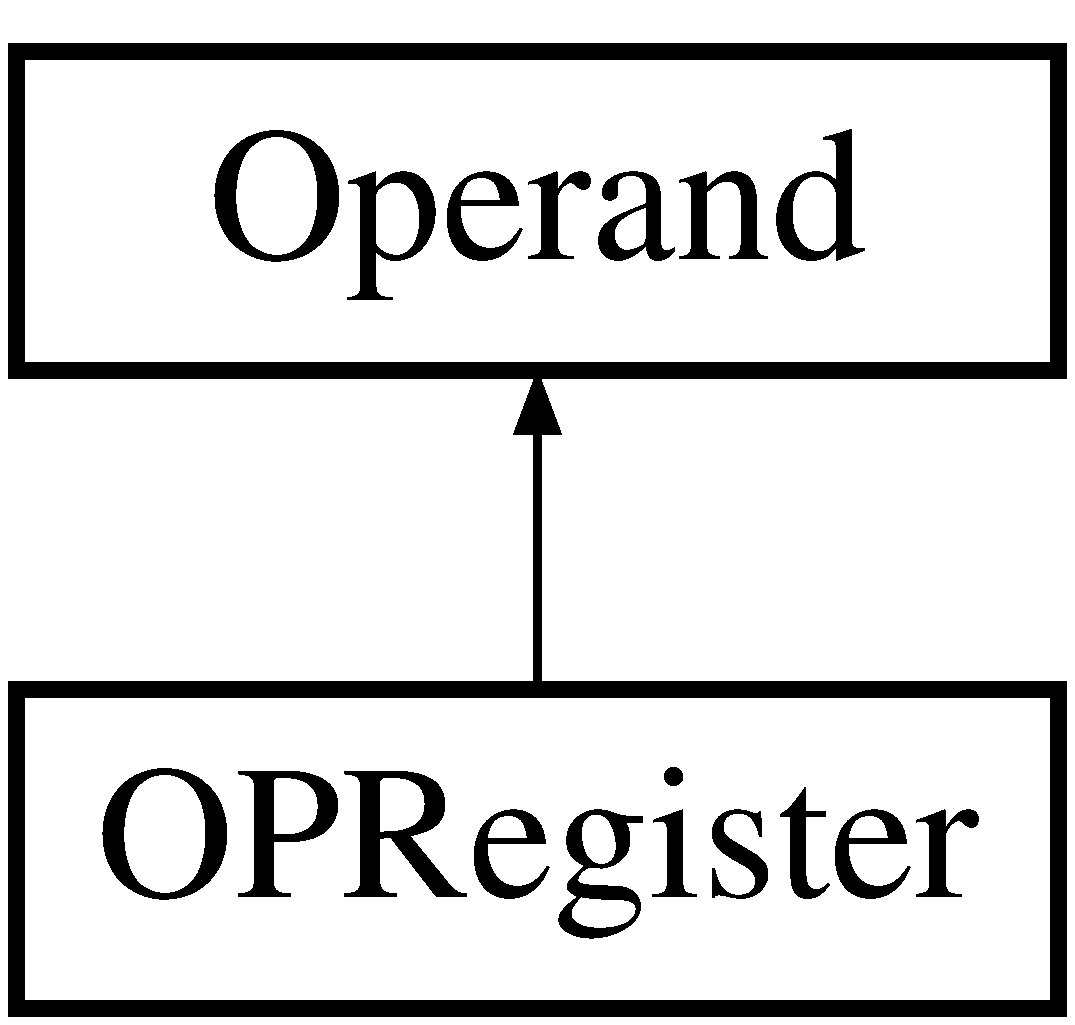
\includegraphics[height=2.000000cm]{class_o_p_register}
\end{center}
\end{figure}
\subsection*{Public Member Functions}
\begin{DoxyCompactItemize}
\item 
\mbox{\Hypertarget{class_o_p_register_a896eb65f36bf615ccfa74541de23858f}\label{class_o_p_register_a896eb65f36bf615ccfa74541de23858f}} 
\mbox{\hyperlink{class_o_p_register_a896eb65f36bf615ccfa74541de23858f}{O\+P\+Register}} (string, t\+\_\+\+Src\+\_\+\+Dst)
\begin{DoxyCompactList}\small\item\em Constructor of the Register class. \end{DoxyCompactList}\item 
\mbox{\Hypertarget{class_o_p_register_ad75c23d1db7c149c20cbc8bb01c6df59}\label{class_o_p_register_ad75c23d1db7c149c20cbc8bb01c6df59}} 
\mbox{\hyperlink{class_o_p_register_ad75c23d1db7c149c20cbc8bb01c6df59}{O\+P\+Register}} (string, int, t\+\_\+\+Src\+\_\+\+Dst)
\begin{DoxyCompactList}\small\item\em Constructor of the Register class. \end{DoxyCompactList}\item 
\mbox{\Hypertarget{class_o_p_register_a3c9786680764ada47370d469790b8178}\label{class_o_p_register_a3c9786680764ada47370d469790b8178}} 
{\bfseries O\+P\+Register} (int, t\+\_\+\+Src\+\_\+\+Dst)
\item 
\mbox{\Hypertarget{class_o_p_register_aedab3bc5a2eecd0d02771fb6b37d73fe}\label{class_o_p_register_aedab3bc5a2eecd0d02771fb6b37d73fe}} 
virtual \mbox{\hyperlink{class_o_p_register_aedab3bc5a2eecd0d02771fb6b37d73fe}{$\sim$\+O\+P\+Register}} ()
\begin{DoxyCompactList}\small\item\em Destructor of the Register class. \end{DoxyCompactList}\item 
int \mbox{\hyperlink{class_o_p_register_acd1c47e67de36adf6b1b88c0a4760b7e}{get\+\_\+reg\+\_\+num}} ()
\begin{DoxyCompactList}\small\item\em Get the number in the Register name. \end{DoxyCompactList}\item 
\mbox{\Hypertarget{class_o_p_register_a1465b14515c02816c15dd1e2b244a4f2}\label{class_o_p_register_a1465b14515c02816c15dd1e2b244a4f2}} 
void \mbox{\hyperlink{class_o_p_register_a1465b14515c02816c15dd1e2b244a4f2}{set\+\_\+reg\+\_\+num}} (int)
\begin{DoxyCompactList}\small\item\em set the Register value setter of the Register \end{DoxyCompactList}\item 
virtual string \mbox{\hyperlink{class_o_p_register_a3f9f6cad40b83eee3f88a2e84a0ccffa}{get\+\_\+op}} ()
\begin{DoxyCompactList}\small\item\em Get the operand value. \end{DoxyCompactList}\item 
virtual t\+\_\+\+Op\+Type \mbox{\hyperlink{class_o_p_register_a1be03d6e6422510a1fd12d1f13dfd601}{get\+\_\+op\+\_\+type}} ()
\begin{DoxyCompactList}\small\item\em get the operator type \end{DoxyCompactList}\item 
virtual string \mbox{\hyperlink{class_o_p_register_a9f55bdff75224fb18973a9e913a4022f}{to\+\_\+string}} ()
\begin{DoxyCompactList}\small\item\em tostring \end{DoxyCompactList}\item 
\mbox{\Hypertarget{class_o_p_register_a3cceb6c804e4fe1187de7eb47c21a285}\label{class_o_p_register_a3cceb6c804e4fe1187de7eb47c21a285}} 
virtual void \mbox{\hyperlink{class_o_p_register_a3cceb6c804e4fe1187de7eb47c21a285}{set\+\_\+op}} (string)
\begin{DoxyCompactList}\small\item\em set the operand value setter of the operand \end{DoxyCompactList}\item 
\mbox{\Hypertarget{class_o_p_register_a23b5061c12e99d3bd320038e643eb247}\label{class_o_p_register_a23b5061c12e99d3bd320038e643eb247}} 
void \mbox{\hyperlink{class_o_p_register_a23b5061c12e99d3bd320038e643eb247}{set\+\_\+type}} (t\+\_\+\+Src\+\_\+\+Dst)
\begin{DoxyCompactList}\small\item\em set the type of the register setter of the register type \end{DoxyCompactList}\item 
\mbox{\Hypertarget{class_o_p_register_a7748867306b20ca99c0955b376789777}\label{class_o_p_register_a7748867306b20ca99c0955b376789777}} 
t\+\_\+\+Src\+\_\+\+Dst \mbox{\hyperlink{class_o_p_register_a7748867306b20ca99c0955b376789777}{get\+\_\+type}} ()
\begin{DoxyCompactList}\small\item\em get the type of the register getter of the register type \end{DoxyCompactList}\end{DoxyCompactItemize}
\subsection*{Additional Inherited Members}


\subsection{Detailed Description}
class representing a Register herited by \mbox{\hyperlink{class_operand}{Operand}} 

\subsection{Member Function Documentation}
\mbox{\Hypertarget{class_o_p_register_a3f9f6cad40b83eee3f88a2e84a0ccffa}\label{class_o_p_register_a3f9f6cad40b83eee3f88a2e84a0ccffa}} 
\index{O\+P\+Register@{O\+P\+Register}!get\+\_\+op@{get\+\_\+op}}
\index{get\+\_\+op@{get\+\_\+op}!O\+P\+Register@{O\+P\+Register}}
\subsubsection{\texorpdfstring{get\+\_\+op()}{get\_op()}}
{\footnotesize\ttfamily virtual string O\+P\+Register\+::get\+\_\+op (\begin{DoxyParamCaption}{ }\end{DoxyParamCaption})\hspace{0.3cm}{\ttfamily [virtual]}}



Get the operand value. 

\begin{DoxyReturn}{Returns}
return the string of the register 
\end{DoxyReturn}


Implements \mbox{\hyperlink{class_operand_a2bf3ad8b34d39cb35ff743ffcc0f4675}{Operand}}.

\mbox{\Hypertarget{class_o_p_register_a1be03d6e6422510a1fd12d1f13dfd601}\label{class_o_p_register_a1be03d6e6422510a1fd12d1f13dfd601}} 
\index{O\+P\+Register@{O\+P\+Register}!get\+\_\+op\+\_\+type@{get\+\_\+op\+\_\+type}}
\index{get\+\_\+op\+\_\+type@{get\+\_\+op\+\_\+type}!O\+P\+Register@{O\+P\+Register}}
\subsubsection{\texorpdfstring{get\+\_\+op\+\_\+type()}{get\_op\_type()}}
{\footnotesize\ttfamily virtual t\+\_\+\+Op\+Type O\+P\+Register\+::get\+\_\+op\+\_\+type (\begin{DoxyParamCaption}{ }\end{DoxyParamCaption})\hspace{0.3cm}{\ttfamily [virtual]}}



get the operator type 

\begin{DoxyReturn}{Returns}
return the \mbox{\hyperlink{class_operand}{Operand}} type as enum 
\end{DoxyReturn}


Implements \mbox{\hyperlink{class_operand_afd469e305a467e2574f34ac9bd6c62b0}{Operand}}.

\mbox{\Hypertarget{class_o_p_register_acd1c47e67de36adf6b1b88c0a4760b7e}\label{class_o_p_register_acd1c47e67de36adf6b1b88c0a4760b7e}} 
\index{O\+P\+Register@{O\+P\+Register}!get\+\_\+reg\+\_\+num@{get\+\_\+reg\+\_\+num}}
\index{get\+\_\+reg\+\_\+num@{get\+\_\+reg\+\_\+num}!O\+P\+Register@{O\+P\+Register}}
\subsubsection{\texorpdfstring{get\+\_\+reg\+\_\+num()}{get\_reg\_num()}}
{\footnotesize\ttfamily int O\+P\+Register\+::get\+\_\+reg\+\_\+num (\begin{DoxyParamCaption}{ }\end{DoxyParamCaption})}



Get the number in the Register name. 

\begin{DoxyReturn}{Returns}
return the number of the Register 
\end{DoxyReturn}
\mbox{\Hypertarget{class_o_p_register_a9f55bdff75224fb18973a9e913a4022f}\label{class_o_p_register_a9f55bdff75224fb18973a9e913a4022f}} 
\index{O\+P\+Register@{O\+P\+Register}!to\+\_\+string@{to\+\_\+string}}
\index{to\+\_\+string@{to\+\_\+string}!O\+P\+Register@{O\+P\+Register}}
\subsubsection{\texorpdfstring{to\+\_\+string()}{to\_string()}}
{\footnotesize\ttfamily virtual string O\+P\+Register\+::to\+\_\+string (\begin{DoxyParamCaption}{ }\end{DoxyParamCaption})\hspace{0.3cm}{\ttfamily [virtual]}}



tostring 

\begin{DoxyReturn}{Returns}
return the Object as string 
\end{DoxyReturn}


Implements \mbox{\hyperlink{class_operand_a28aed96d5fafee66be81c30c1435ad00}{Operand}}.



The documentation for this class was generated from the following file\+:\begin{DoxyCompactItemize}
\item 
include/\mbox{\hyperlink{_o_p_register_8h}{O\+P\+Register.\+h}}\end{DoxyCompactItemize}

\hypertarget{class_program}{}\section{Program Class Reference}
\label{class_program}\index{Program@{Program}}


class representing a program as list  




{\ttfamily \#include $<$Program.\+h$>$}

\subsection*{Public Member Functions}
\begin{DoxyCompactItemize}
\item 
\mbox{\Hypertarget{class_program_aaefaa0df08f3484476fc4d61e97acbdc}\label{class_program_aaefaa0df08f3484476fc4d61e97acbdc}} 
\mbox{\hyperlink{class_program_aaefaa0df08f3484476fc4d61e97acbdc}{Program}} ()
\begin{DoxyCompactList}\small\item\em Empty constructor of a program. \end{DoxyCompactList}\item 
\mbox{\Hypertarget{class_program_a9918fe797bf830c47a652c81f449c35c}\label{class_program_a9918fe797bf830c47a652c81f449c35c}} 
\mbox{\hyperlink{class_program_a9918fe797bf830c47a652c81f449c35c}{Program}} (\mbox{\hyperlink{class_program}{Program}} const \&otherprogram)
\begin{DoxyCompactList}\small\item\em Copy constructor of a program. \end{DoxyCompactList}\item 
\mbox{\Hypertarget{class_program_aabe3dfc72075de14b189b22b0e33ff23}\label{class_program_aabe3dfc72075de14b189b22b0e33ff23}} 
\mbox{\hyperlink{class_program_aabe3dfc72075de14b189b22b0e33ff23}{Program}} (string const file)
\begin{DoxyCompactList}\small\item\em Constructor with the input file of program. \end{DoxyCompactList}\item 
\mbox{\Hypertarget{class_program_a986aef1c50e1d338a3315a47ba6df549}\label{class_program_a986aef1c50e1d338a3315a47ba6df549}} 
\mbox{\hyperlink{class_program_a986aef1c50e1d338a3315a47ba6df549}{$\sim$\+Program}} ()
\begin{DoxyCompactList}\small\item\em Destructor of program. \end{DoxyCompactList}\item 
\mbox{\Hypertarget{class_program_a90e1c506dffd5756133f70811f6117d9}\label{class_program_a90e1c506dffd5756133f70811f6117d9}} 
void \mbox{\hyperlink{class_program_a90e1c506dffd5756133f70811f6117d9}{add\+\_\+line}} (\mbox{\hyperlink{class_line}{Line}} $\ast$newline)
\begin{DoxyCompactList}\small\item\em Add a line at the end of the program. \end{DoxyCompactList}\item 
\mbox{\Hypertarget{class_program_a7adb0709f1a9f3ed63e861cc7f02d308}\label{class_program_a7adb0709f1a9f3ed63e861cc7f02d308}} 
int \mbox{\hyperlink{class_program_a7adb0709f1a9f3ed63e861cc7f02d308}{add\+\_\+line\+\_\+at}} (\mbox{\hyperlink{class_line}{Line}} $\ast$newline, int position)
\begin{DoxyCompactList}\small\item\em Add a line to the program with position as index. \end{DoxyCompactList}\item 
\mbox{\Hypertarget{class_program_aabea8add836e10a384b63e2f293ece23}\label{class_program_aabea8add836e10a384b63e2f293ece23}} 
void \mbox{\hyperlink{class_program_aabea8add836e10a384b63e2f293ece23}{exchange\+\_\+line}} (int line1, int line2)
\begin{DoxyCompactList}\small\item\em Reverse two lines which are at the index line1 and line2. \end{DoxyCompactList}\item 
\mbox{\Hypertarget{class_program_a3c1399ac5ed69e5c152f1a2cc1e644d4}\label{class_program_a3c1399ac5ed69e5c152f1a2cc1e644d4}} 
void \mbox{\hyperlink{class_program_a3c1399ac5ed69e5c152f1a2cc1e644d4}{display}} ()
\begin{DoxyCompactList}\small\item\em display the program \end{DoxyCompactList}\item 
\mbox{\Hypertarget{class_program_a1adce5c1fc414a378e4b87f1d4b535e1}\label{class_program_a1adce5c1fc414a378e4b87f1d4b535e1}} 
void \mbox{\hyperlink{class_program_a1adce5c1fc414a378e4b87f1d4b535e1}{del\+\_\+line}} (int index)
\begin{DoxyCompactList}\small\item\em Delete the line at the given index in the program. \end{DoxyCompactList}\item 
\mbox{\Hypertarget{class_program_ae897b48e1e1be99578440eb6a38a3a0d}\label{class_program_ae897b48e1e1be99578440eb6a38a3a0d}} 
\mbox{\hyperlink{class_line}{Line}} $\ast$ \mbox{\hyperlink{class_program_ae897b48e1e1be99578440eb6a38a3a0d}{find\+\_\+line}} (int index)
\begin{DoxyCompactList}\small\item\em gives the line that corresponds to the index \end{DoxyCompactList}\item 
\mbox{\Hypertarget{class_program_a190f24ecadca14d748408c352aabc219}\label{class_program_a190f24ecadca14d748408c352aabc219}} 
int \mbox{\hyperlink{class_program_a190f24ecadca14d748408c352aabc219}{size}} ()
\begin{DoxyCompactList}\small\item\em get the length of the program \end{DoxyCompactList}\item 
void \mbox{\hyperlink{class_program_a3db3e17c96bb809c3e6f81b8bc22ee20}{in\+\_\+file}} (string const filename)
\begin{DoxyCompactList}\small\item\em returns the dependance betwen the two given instructions \end{DoxyCompactList}\item 
\mbox{\Hypertarget{class_program_aff32c461ae544453df5d55f475b3da22}\label{class_program_aff32c461ae544453df5d55f475b3da22}} 
bool \mbox{\hyperlink{class_program_aff32c461ae544453df5d55f475b3da22}{is\+\_\+empty}} ()
\begin{DoxyCompactList}\small\item\em return true if the program is Empty \end{DoxyCompactList}\item 
\mbox{\Hypertarget{class_program_aa2111257b1f690520316e4831e55798d}\label{class_program_aa2111257b1f690520316e4831e55798d}} 
void \mbox{\hyperlink{class_program_aa2111257b1f690520316e4831e55798d}{comput\+\_\+function}} ()
\begin{DoxyCompactList}\small\item\em calculate the functions of the program \end{DoxyCompactList}\item 
\mbox{\Hypertarget{class_program_aa85073d3bd6782af3759f4a2961ae80f}\label{class_program_aa85073d3bd6782af3759f4a2961ae80f}} 
int \mbox{\hyperlink{class_program_aa85073d3bd6782af3759f4a2961ae80f}{nbr\+\_\+func}} ()
\begin{DoxyCompactList}\small\item\em get the number of functions in the program \end{DoxyCompactList}\item 
\mbox{\Hypertarget{class_program_aea6d5c7367bbee48ec5cbb295ef6fd5f}\label{class_program_aea6d5c7367bbee48ec5cbb295ef6fd5f}} 
\mbox{\hyperlink{class_function}{Function}} $\ast$ \mbox{\hyperlink{class_program_aea6d5c7367bbee48ec5cbb295ef6fd5f}{get\+\_\+function}} (int index)
\begin{DoxyCompactList}\small\item\em returns the function of index index in the list \+\_\+myfunc \end{DoxyCompactList}\item 
\mbox{\Hypertarget{class_program_a1cef65227311c68a2e81c89dcbc16914}\label{class_program_a1cef65227311c68a2e81c89dcbc16914}} 
void \mbox{\hyperlink{class_program_a1cef65227311c68a2e81c89dcbc16914}{flush}} ()
\begin{DoxyCompactList}\small\item\em empty the program \end{DoxyCompactList}\item 
\mbox{\Hypertarget{class_program_a0d1d9386925418b5fd0a09bf5de16208}\label{class_program_a0d1d9386925418b5fd0a09bf5de16208}} 
void \mbox{\hyperlink{class_program_a0d1d9386925418b5fd0a09bf5de16208}{comput\+\_\+\+C\+FG}} ()
\begin{DoxyCompactList}\small\item\em calculate the C\+FG associated with each function of the program \end{DoxyCompactList}\item 
\mbox{\Hypertarget{class_program_a69ddee195c76bff05733d927e315f319}\label{class_program_a69ddee195c76bff05733d927e315f319}} 
\mbox{\hyperlink{class_cfg}{Cfg}} $\ast$ \mbox{\hyperlink{class_program_a69ddee195c76bff05733d927e315f319}{get\+\_\+\+C\+FG}} (int index)
\begin{DoxyCompactList}\small\item\em returns the C\+FG of index index in the list \+\_\+my\+C\+FG \end{DoxyCompactList}\end{DoxyCompactItemize}


\subsection{Detailed Description}
class representing a program as list 

\subsection{Member Function Documentation}
\mbox{\Hypertarget{class_program_a3db3e17c96bb809c3e6f81b8bc22ee20}\label{class_program_a3db3e17c96bb809c3e6f81b8bc22ee20}} 
\index{Program@{Program}!in\+\_\+file@{in\+\_\+file}}
\index{in\+\_\+file@{in\+\_\+file}!Program@{Program}}
\subsubsection{\texorpdfstring{in\+\_\+file()}{in\_file()}}
{\footnotesize\ttfamily void Program\+::in\+\_\+file (\begin{DoxyParamCaption}\item[{string const}]{filename }\end{DoxyParamCaption})}



returns the dependance betwen the two given instructions 

\begin{DoxyReturn}{Returns}
returns the dependance in the enum formatwrite the programme into a file 
\end{DoxyReturn}


The documentation for this class was generated from the following file\+:\begin{DoxyCompactItemize}
\item 
include/\mbox{\hyperlink{_program_8h}{Program.\+h}}\end{DoxyCompactItemize}

\hypertarget{structs___profile}{}\section{s\+\_\+\+Profile Struct Reference}
\label{structs___profile}\index{s\+\_\+\+Profile@{s\+\_\+\+Profile}}


Structure allowing to add caracteristics to an operator.  




{\ttfamily \#include $<$Enum\+\_\+type.\+h$>$}

\subsection*{Public Attributes}
\begin{DoxyCompactItemize}
\item 
\mbox{\Hypertarget{structs___profile_a3debabafa904b8f4c5e7bf2bda2a5e60}\label{structs___profile_a3debabafa904b8f4c5e7bf2bda2a5e60}} 
t\+\_\+\+Operator {\bfseries op}
\item 
\mbox{\Hypertarget{structs___profile_ab9f52013690834dd36766d356c90c449}\label{structs___profile_ab9f52013690834dd36766d356c90c449}} 
std\+::string {\bfseries nom}
\item 
\mbox{\Hypertarget{structs___profile_ae8153795530389f76f6c56bdeac40d46}\label{structs___profile_ae8153795530389f76f6c56bdeac40d46}} 
t\+\_\+\+Format {\bfseries format}
\item 
\mbox{\Hypertarget{structs___profile_a2a8c53bcb4fb28c3aa368a27954d9b1b}\label{structs___profile_a2a8c53bcb4fb28c3aa368a27954d9b1b}} 
t\+\_\+\+Inst {\bfseries type}
\item 
\mbox{\Hypertarget{structs___profile_a7930c41fdfa4249a1c147edf7ac68822}\label{structs___profile_a7930c41fdfa4249a1c147edf7ac68822}} 
int {\bfseries nb\+\_\+oper}
\end{DoxyCompactItemize}


\subsection{Detailed Description}
Structure allowing to add caracteristics to an operator. 

The documentation for this struct was generated from the following file\+:\begin{DoxyCompactItemize}
\item 
include/Enum\+\_\+type.\+h\end{DoxyCompactItemize}

\chapter{File Documentation}
\hypertarget{_basic__block_8h}{}\section{include/\+Basic\+\_\+block.h File Reference}
\label{_basic__block_8h}\index{include/\+Basic\+\_\+block.\+h@{include/\+Basic\+\_\+block.\+h}}


\mbox{\hyperlink{class_basic__block}{Basic\+\_\+block}} class.  


{\ttfamily \#include $<$Line.\+h$>$}\newline
{\ttfamily \#include $<$Instruction.\+h$>$}\newline
{\ttfamily \#include $<$string$>$}\newline
{\ttfamily \#include $<$stdio.\+h$>$}\newline
{\ttfamily \#include $<$Enum\+\_\+type.\+h$>$}\newline
{\ttfamily \#include $<$fstream$>$}\newline
{\ttfamily \#include $<$vector$>$}\newline
{\ttfamily \#include $<$list$>$}\newline
{\ttfamily \#include $<$Dfg.\+h$>$}\newline
{\ttfamily \#include $<$Node\+\_\+dfg.\+h$>$}\newline
\subsection*{Classes}
\begin{DoxyCompactItemize}
\item 
class \mbox{\hyperlink{class_basic__block}{Basic\+\_\+block}}
\begin{DoxyCompactList}\small\item\em class representing a \mbox{\hyperlink{class_basic__block}{Basic\+\_\+block}} of a fonction \end{DoxyCompactList}\end{DoxyCompactItemize}


\subsection{Detailed Description}
\mbox{\hyperlink{class_basic__block}{Basic\+\_\+block}} class. 

\begin{DoxyAuthor}{Author}
Hajjem, Heydemann 
\end{DoxyAuthor}

\hypertarget{_cfg_8h}{}\section{include/\+Cfg.h File Reference}
\label{_cfg_8h}\index{include/\+Cfg.\+h@{include/\+Cfg.\+h}}


\mbox{\hyperlink{class_cfg}{Cfg}} class.  


{\ttfamily \#include $<$Basic\+\_\+block.\+h$>$}\newline
{\ttfamily \#include $<$string$>$}\newline
{\ttfamily \#include $<$stdio.\+h$>$}\newline
{\ttfamily \#include $<$Label.\+h$>$}\newline
{\ttfamily \#include $<$Enum\+\_\+type.\+h$>$}\newline
{\ttfamily \#include $<$list$>$}\newline
{\ttfamily \#include $<$fstream$>$}\newline
\subsection*{Classes}
\begin{DoxyCompactItemize}
\item 
class \mbox{\hyperlink{class_cfg}{Cfg}}
\begin{DoxyCompactList}\small\item\em class representing control flow graph \end{DoxyCompactList}\end{DoxyCompactItemize}


\subsection{Detailed Description}
\mbox{\hyperlink{class_cfg}{Cfg}} class. 

\begin{DoxyAuthor}{Author}
Hajjem 
\end{DoxyAuthor}

\hypertarget{_dfg_8h}{}\section{include/\+Dfg.h File Reference}
\label{_dfg_8h}\index{include/\+Dfg.\+h@{include/\+Dfg.\+h}}


\mbox{\hyperlink{class_dfg}{Dfg}} class.  


{\ttfamily \#include $<$Node\+\_\+dfg.\+h$>$}\newline
{\ttfamily \#include $<$Instruction.\+h$>$}\newline
{\ttfamily \#include $<$Enum\+\_\+type.\+h$>$}\newline
{\ttfamily \#include $<$fstream$>$}\newline
{\ttfamily \#include $<$list$>$}\newline
\subsection*{Classes}
\begin{DoxyCompactItemize}
\item 
class \mbox{\hyperlink{class_dfg}{Dfg}}
\begin{DoxyCompactList}\small\item\em class representing a \mbox{\hyperlink{class_dfg}{Dfg}} of a Basic block, a data flow graph that is to be used to calculate the critical path and schedule code \end{DoxyCompactList}\end{DoxyCompactItemize}


\subsection{Detailed Description}
\mbox{\hyperlink{class_dfg}{Dfg}} class. 


\hypertarget{_directive_8h}{}\section{include/\+Directive.h File Reference}
\label{_directive_8h}\index{include/\+Directive.\+h@{include/\+Directive.\+h}}


\mbox{\hyperlink{class_directive}{Directive}} class.  


{\ttfamily \#include $<$iostream$>$}\newline
{\ttfamily \#include $<$string$>$}\newline
{\ttfamily \#include $<$Enum\+\_\+type.\+h$>$}\newline
{\ttfamily \#include $<$Line.\+h$>$}\newline
\subsection*{Classes}
\begin{DoxyCompactItemize}
\item 
class \mbox{\hyperlink{class_directive}{Directive}}
\begin{DoxyCompactList}\small\item\em class representing an \mbox{\hyperlink{class_directive}{Directive}} herited by \mbox{\hyperlink{class_line}{Line}} \end{DoxyCompactList}\end{DoxyCompactItemize}
\subsection*{Functions}
\begin{DoxyCompactItemize}
\item 
\mbox{\Hypertarget{_directive_8h_a0f34d943225eea7b4ffdb6107a79fff1}\label{_directive_8h_a0f34d943225eea7b4ffdb6107a79fff1}} 
\mbox{\hyperlink{class_directive}{Directive}} $\ast$ \mbox{\hyperlink{_directive_8h_a0f34d943225eea7b4ffdb6107a79fff1}{get\+Directive}} (\mbox{\hyperlink{class_line}{Line}} $\ast$l)
\begin{DoxyCompactList}\small\item\em returns the \mbox{\hyperlink{class_directive}{Directive}} associated to the line, if the line is a directive, nullptr otherwise \end{DoxyCompactList}\end{DoxyCompactItemize}


\subsection{Detailed Description}
\mbox{\hyperlink{class_directive}{Directive}} class. 

\begin{DoxyAuthor}{Author}
Hajjem 
\end{DoxyAuthor}

\hypertarget{_function_8h}{}\section{include/\+Function.h File Reference}
\label{_function_8h}\index{include/\+Function.\+h@{include/\+Function.\+h}}


\mbox{\hyperlink{class_function}{Function}} class.  


{\ttfamily \#include $<$Line.\+h$>$}\newline
{\ttfamily \#include $<$Basic\+\_\+block.\+h$>$}\newline
{\ttfamily \#include $<$Loop.\+h$>$}\newline
{\ttfamily \#include $<$Instruction.\+h$>$}\newline
{\ttfamily \#include $<$string$>$}\newline
{\ttfamily \#include $<$stdio.\+h$>$}\newline
{\ttfamily \#include $<$Label.\+h$>$}\newline
{\ttfamily \#include $<$Enum\+\_\+type.\+h$>$}\newline
{\ttfamily \#include $<$list$>$}\newline
{\ttfamily \#include $<$Cfg.\+h$>$}\newline
{\ttfamily \#include $<$fstream$>$}\newline
\subsection*{Classes}
\begin{DoxyCompactItemize}
\item 
class \mbox{\hyperlink{class_function}{Function}}
\begin{DoxyCompactList}\small\item\em class representing a \mbox{\hyperlink{class_function}{Function}} in a program \end{DoxyCompactList}\end{DoxyCompactItemize}


\subsection{Detailed Description}
\mbox{\hyperlink{class_function}{Function}} class. 

\begin{DoxyAuthor}{Author}
Hajjem, Heydemann 
\end{DoxyAuthor}

\hypertarget{_instruction_8h}{}\section{include/\+Instruction.h File Reference}
\label{_instruction_8h}\index{include/\+Instruction.\+h@{include/\+Instruction.\+h}}


\mbox{\hyperlink{class_instruction}{Instruction}} class.  


{\ttfamily \#include $<$Operand.\+h$>$}\newline
{\ttfamily \#include $<$string$>$}\newline
{\ttfamily \#include $<$O\+P\+Expression.\+h$>$}\newline
{\ttfamily \#include $<$O\+P\+Immediate.\+h$>$}\newline
{\ttfamily \#include $<$O\+P\+Label.\+h$>$}\newline
{\ttfamily \#include $<$Line.\+h$>$}\newline
{\ttfamily \#include $<$O\+P\+Register.\+h$>$}\newline
{\ttfamily \#include $<$Enum\+\_\+type.\+h$>$}\newline
{\ttfamily \#include $<$list$>$}\newline
\subsection*{Classes}
\begin{DoxyCompactItemize}
\item 
struct \mbox{\hyperlink{structdep}{dep}}
\item 
class \mbox{\hyperlink{class_instruction}{Instruction}}
\begin{DoxyCompactList}\small\item\em class representing an instruction which herited by \mbox{\hyperlink{class_line}{Line}} \end{DoxyCompactList}\end{DoxyCompactItemize}
\subsection*{Functions}
\begin{DoxyCompactItemize}
\item 
\mbox{\Hypertarget{_instruction_8h_a8b4a12440add75fe3ebf3a5d3ed4ee8e}\label{_instruction_8h_a8b4a12440add75fe3ebf3a5d3ed4ee8e}} 
\mbox{\hyperlink{class_instruction}{Instruction}} $\ast$ \mbox{\hyperlink{_instruction_8h_a8b4a12440add75fe3ebf3a5d3ed4ee8e}{get\+Inst}} (\mbox{\hyperlink{class_line}{Line}} $\ast$l)
\begin{DoxyCompactList}\small\item\em returns the instruction associated to the line, if the line is an instruction, nullptr otherwise \end{DoxyCompactList}\item 
int \mbox{\hyperlink{_instruction_8h_a51ba1f2ef8910a3a40a3bf9923286e7c}{delai}} (t\+\_\+\+Inst t1, t\+\_\+\+Inst t2)
\begin{DoxyCompactList}\small\item\em retourne le délai induit par une dépendance R\+AW entre i1 et i2 (i1 -\/$>$ i2) avec i1 de type t1 et i2 de type t2 \end{DoxyCompactList}\end{DoxyCompactItemize}


\subsection{Detailed Description}
\mbox{\hyperlink{class_instruction}{Instruction}} class. 



\subsection{Function Documentation}
\mbox{\Hypertarget{_instruction_8h_a51ba1f2ef8910a3a40a3bf9923286e7c}\label{_instruction_8h_a51ba1f2ef8910a3a40a3bf9923286e7c}} 
\index{Instruction.\+h@{Instruction.\+h}!delai@{delai}}
\index{delai@{delai}!Instruction.\+h@{Instruction.\+h}}
\subsubsection{\texorpdfstring{delai()}{delai()}}
{\footnotesize\ttfamily int delai (\begin{DoxyParamCaption}\item[{t\+\_\+\+Inst}]{t1,  }\item[{t\+\_\+\+Inst}]{t2 }\end{DoxyParamCaption})}



retourne le délai induit par une dépendance R\+AW entre i1 et i2 (i1 -\/$>$ i2) avec i1 de type t1 et i2 de type t2 


\hypertarget{_label_8h}{}\section{include/\+Label.h File Reference}
\label{_label_8h}\index{include/\+Label.\+h@{include/\+Label.\+h}}


\mbox{\hyperlink{class_label}{Label}} class.  


{\ttfamily \#include $<$iostream$>$}\newline
{\ttfamily \#include $<$string$>$}\newline
{\ttfamily \#include $<$Enum\+\_\+type.\+h$>$}\newline
{\ttfamily \#include $<$Line.\+h$>$}\newline
\subsection*{Classes}
\begin{DoxyCompactItemize}
\item 
class \mbox{\hyperlink{class_label}{Label}}
\begin{DoxyCompactList}\small\item\em class representing an \mbox{\hyperlink{class_label}{Label}} herited by \mbox{\hyperlink{class_line}{Line}} \end{DoxyCompactList}\end{DoxyCompactItemize}
\subsection*{Functions}
\begin{DoxyCompactItemize}
\item 
\mbox{\Hypertarget{_label_8h_a1b9f6053866196b9132c6af17820ce00}\label{_label_8h_a1b9f6053866196b9132c6af17820ce00}} 
\mbox{\hyperlink{class_label}{Label}} $\ast$ \mbox{\hyperlink{_label_8h_a1b9f6053866196b9132c6af17820ce00}{get\+Label}} (\mbox{\hyperlink{class_line}{Line}} $\ast$l)
\begin{DoxyCompactList}\small\item\em returns the \mbox{\hyperlink{class_label}{Label}} associated to the line if the line is a label, nullptr otherwise \end{DoxyCompactList}\end{DoxyCompactItemize}


\subsection{Detailed Description}
\mbox{\hyperlink{class_label}{Label}} class. 

\begin{DoxyAuthor}{Author}
Hajjem 
\end{DoxyAuthor}

\hypertarget{_line_8h}{}\section{include/\+Line.h File Reference}
\label{_line_8h}\index{include/\+Line.\+h@{include/\+Line.\+h}}


\mbox{\hyperlink{class_line}{Line}} class.  


{\ttfamily \#include $<$iostream$>$}\newline
{\ttfamily \#include $<$string$>$}\newline
{\ttfamily \#include $<$Enum\+\_\+type.\+h$>$}\newline
\subsection*{Classes}
\begin{DoxyCompactItemize}
\item 
class \mbox{\hyperlink{class_line}{Line}}
\begin{DoxyCompactList}\small\item\em Abstract class representing an \mbox{\hyperlink{class_line}{Line}}. \end{DoxyCompactList}\end{DoxyCompactItemize}


\subsection{Detailed Description}
\mbox{\hyperlink{class_line}{Line}} class. 


\hypertarget{_loop_8h}{}\section{include/\+Loop.h File Reference}
\label{_loop_8h}\index{include/\+Loop.\+h@{include/\+Loop.\+h}}


\mbox{\hyperlink{class_function}{Function}} class.  


{\ttfamily \#include $<$Line.\+h$>$}\newline
{\ttfamily \#include $<$Basic\+\_\+block.\+h$>$}\newline
{\ttfamily \#include $<$Instruction.\+h$>$}\newline
{\ttfamily \#include $<$string$>$}\newline
{\ttfamily \#include $<$stdio.\+h$>$}\newline
{\ttfamily \#include $<$Label.\+h$>$}\newline
{\ttfamily \#include $<$Enum\+\_\+type.\+h$>$}\newline
{\ttfamily \#include $<$list$>$}\newline
{\ttfamily \#include $<$Cfg.\+h$>$}\newline
{\ttfamily \#include $<$fstream$>$}\newline
\subsection*{Classes}
\begin{DoxyCompactItemize}
\item 
class \mbox{\hyperlink{class_loop}{Loop}}
\begin{DoxyCompactList}\small\item\em class representing a \mbox{\hyperlink{class_loop}{Loop}} in a function \end{DoxyCompactList}\end{DoxyCompactItemize}


\subsection{Detailed Description}
\mbox{\hyperlink{class_function}{Function}} class. 

\begin{DoxyAuthor}{Author}
Heydemann 
\end{DoxyAuthor}

\hypertarget{_node__dfg_8h}{}\section{include/\+Node\+\_\+dfg.h File Reference}
\label{_node__dfg_8h}\index{include/\+Node\+\_\+dfg.\+h@{include/\+Node\+\_\+dfg.\+h}}


\mbox{\hyperlink{class_node__dfg}{Node\+\_\+dfg}} class.  


{\ttfamily \#include $<$Basic\+\_\+block.\+h$>$}\newline
{\ttfamily \#include $<$string$>$}\newline
{\ttfamily \#include $<$stdio.\+h$>$}\newline
{\ttfamily \#include $<$Label.\+h$>$}\newline
{\ttfamily \#include $<$Enum\+\_\+type.\+h$>$}\newline
\subsection*{Classes}
\begin{DoxyCompactItemize}
\item 
struct \mbox{\hyperlink{struct_arc__t}{Arc\+\_\+t}}
\item 
class \mbox{\hyperlink{class_node__dfg}{Node\+\_\+dfg}}
\begin{DoxyCompactList}\small\item\em class representing a node of data flow graph \end{DoxyCompactList}\end{DoxyCompactItemize}


\subsection{Detailed Description}
\mbox{\hyperlink{class_node__dfg}{Node\+\_\+dfg}} class. 


\hypertarget{_operand_8h}{}\section{include/\+Operand.h File Reference}
\label{_operand_8h}\index{include/\+Operand.\+h@{include/\+Operand.\+h}}


\mbox{\hyperlink{class_operand}{Operand}} class.  


{\ttfamily \#include $<$iostream$>$}\newline
{\ttfamily \#include $<$string$>$}\newline
{\ttfamily \#include $<$Enum\+\_\+type.\+h$>$}\newline
\subsection*{Classes}
\begin{DoxyCompactItemize}
\item 
class \mbox{\hyperlink{class_operand}{Operand}}
\begin{DoxyCompactList}\small\item\em Abstract class representing an operand. \end{DoxyCompactList}\end{DoxyCompactItemize}


\subsection{Detailed Description}
\mbox{\hyperlink{class_operand}{Operand}} class. 

\begin{DoxyAuthor}{Author}
Hajjem 
\end{DoxyAuthor}

\hypertarget{_o_p_expression_8h}{}\section{include/\+O\+P\+Expression.h File Reference}
\label{_o_p_expression_8h}\index{include/\+O\+P\+Expression.\+h@{include/\+O\+P\+Expression.\+h}}


\mbox{\hyperlink{class_o_p_expression}{O\+P\+Expression}} class.  


{\ttfamily \#include $<$iostream$>$}\newline
{\ttfamily \#include $<$string$>$}\newline
{\ttfamily \#include $<$Operand.\+h$>$}\newline
{\ttfamily \#include $<$Enum\+\_\+type.\+h$>$}\newline
\subsection*{Classes}
\begin{DoxyCompactItemize}
\item 
class \mbox{\hyperlink{class_o_p_expression}{O\+P\+Expression}}
\begin{DoxyCompactList}\small\item\em class representing an expression herited by \mbox{\hyperlink{class_operand}{Operand}} \end{DoxyCompactList}\end{DoxyCompactItemize}


\subsection{Detailed Description}
\mbox{\hyperlink{class_o_p_expression}{O\+P\+Expression}} class. 

\begin{DoxyAuthor}{Author}
Hajjem 
\end{DoxyAuthor}

\hypertarget{_o_p_immediate_8h}{}\section{include/\+O\+P\+Immediate.h File Reference}
\label{_o_p_immediate_8h}\index{include/\+O\+P\+Immediate.\+h@{include/\+O\+P\+Immediate.\+h}}


\mbox{\hyperlink{class_o_p_immediate}{O\+P\+Immediate}} class.  


{\ttfamily \#include $<$iostream$>$}\newline
{\ttfamily \#include $<$string$>$}\newline
{\ttfamily \#include $<$Operand.\+h$>$}\newline
{\ttfamily \#include $<$Enum\+\_\+type.\+h$>$}\newline
\subsection*{Classes}
\begin{DoxyCompactItemize}
\item 
class \mbox{\hyperlink{class_o_p_immediate}{O\+P\+Immediate}}
\begin{DoxyCompactList}\small\item\em class representing an Immediate herited by \mbox{\hyperlink{class_operand}{Operand}} \end{DoxyCompactList}\end{DoxyCompactItemize}


\subsection{Detailed Description}
\mbox{\hyperlink{class_o_p_immediate}{O\+P\+Immediate}} class. 

\begin{DoxyAuthor}{Author}
Hajjem 
\end{DoxyAuthor}

\hypertarget{_o_p_label_8h}{}\section{include/\+O\+P\+Label.h File Reference}
\label{_o_p_label_8h}\index{include/\+O\+P\+Label.\+h@{include/\+O\+P\+Label.\+h}}


\mbox{\hyperlink{class_o_p_label}{O\+P\+Label}} class.  


{\ttfamily \#include $<$iostream$>$}\newline
{\ttfamily \#include $<$Operand.\+h$>$}\newline
{\ttfamily \#include $<$Enum\+\_\+type.\+h$>$}\newline
{\ttfamily \#include $<$string$>$}\newline
\subsection*{Classes}
\begin{DoxyCompactItemize}
\item 
class \mbox{\hyperlink{class_o_p_label}{O\+P\+Label}}
\begin{DoxyCompactList}\small\item\em class representing a \mbox{\hyperlink{class_label}{Label}} herited by \mbox{\hyperlink{class_operand}{Operand}} \end{DoxyCompactList}\end{DoxyCompactItemize}
\subsection*{Functions}
\begin{DoxyCompactItemize}
\item 
\mbox{\Hypertarget{_o_p_label_8h_a2a54dc70e5071ab362bb95d472986203}\label{_o_p_label_8h_a2a54dc70e5071ab362bb95d472986203}} 
\mbox{\hyperlink{class_o_p_label}{O\+P\+Label}} $\ast$ \mbox{\hyperlink{_o_p_label_8h_a2a54dc70e5071ab362bb95d472986203}{get\+O\+P\+Label}} (\mbox{\hyperlink{class_operand}{Operand}} $\ast$)
\begin{DoxyCompactList}\small\item\em returns the \mbox{\hyperlink{class_o_p_label}{O\+P\+Label}} associated to the \mbox{\hyperlink{class_operand}{Operand}} if it is an \mbox{\hyperlink{class_o_p_label}{O\+P\+Label}}, otherwise returns nullptr \end{DoxyCompactList}\end{DoxyCompactItemize}


\subsection{Detailed Description}
\mbox{\hyperlink{class_o_p_label}{O\+P\+Label}} class. 

\begin{DoxyAuthor}{Author}
Hajjem 
\end{DoxyAuthor}

\hypertarget{_o_p_register_8h}{}\section{include/\+O\+P\+Register.h File Reference}
\label{_o_p_register_8h}\index{include/\+O\+P\+Register.\+h@{include/\+O\+P\+Register.\+h}}


\mbox{\hyperlink{class_o_p_register}{O\+P\+Register}} class.  


{\ttfamily \#include $<$iostream$>$}\newline
{\ttfamily \#include $<$string$>$}\newline
{\ttfamily \#include $<$Operand.\+h$>$}\newline
{\ttfamily \#include $<$Enum\+\_\+type.\+h$>$}\newline
\subsection*{Classes}
\begin{DoxyCompactItemize}
\item 
class \mbox{\hyperlink{class_o_p_register}{O\+P\+Register}}
\begin{DoxyCompactList}\small\item\em class representing a Register herited by \mbox{\hyperlink{class_operand}{Operand}} \end{DoxyCompactList}\end{DoxyCompactItemize}
\subsection*{Functions}
\begin{DoxyCompactItemize}
\item 
\mbox{\Hypertarget{_o_p_register_8h_ab89366a0fcd23fdd394ec0374eda0fac}\label{_o_p_register_8h_ab89366a0fcd23fdd394ec0374eda0fac}} 
\mbox{\hyperlink{class_o_p_register}{O\+P\+Register}} $\ast$ \mbox{\hyperlink{_o_p_register_8h_ab89366a0fcd23fdd394ec0374eda0fac}{get\+O\+P\+Register}} (\mbox{\hyperlink{class_operand}{Operand}} $\ast$)
\begin{DoxyCompactList}\small\item\em returns the \mbox{\hyperlink{class_o_p_register}{O\+P\+Register}} associated to the \mbox{\hyperlink{class_operand}{Operand}} if it is an \mbox{\hyperlink{class_o_p_register}{O\+P\+Register}}, otherwise returns nullptr \end{DoxyCompactList}\end{DoxyCompactItemize}


\subsection{Detailed Description}
\mbox{\hyperlink{class_o_p_register}{O\+P\+Register}} class. 

\begin{DoxyAuthor}{Author}
Hajjem 
\end{DoxyAuthor}

\hypertarget{_program_8h}{}\section{include/\+Program.h File Reference}
\label{_program_8h}\index{include/\+Program.\+h@{include/\+Program.\+h}}


\mbox{\hyperlink{class_program}{Program}} class.  


{\ttfamily \#include $<$Line.\+h$>$}\newline
{\ttfamily \#include $<$Function.\+h$>$}\newline
{\ttfamily \#include $<$Basic\+\_\+block.\+h$>$}\newline
{\ttfamily \#include $<$Instruction.\+h$>$}\newline
{\ttfamily \#include $<$Directive.\+h$>$}\newline
{\ttfamily \#include $<$Cfg.\+h$>$}\newline
{\ttfamily \#include $<$string$>$}\newline
{\ttfamily \#include $<$stdio.\+h$>$}\newline
{\ttfamily \#include $<$Enum\+\_\+type.\+h$>$}\newline
{\ttfamily \#include $<$fstream$>$}\newline
{\ttfamily \#include $<$list$>$}\newline
\subsection*{Classes}
\begin{DoxyCompactItemize}
\item 
class \mbox{\hyperlink{class_program}{Program}}
\begin{DoxyCompactList}\small\item\em class representing a program as list \end{DoxyCompactList}\end{DoxyCompactItemize}


\subsection{Detailed Description}
\mbox{\hyperlink{class_program}{Program}} class. 

\begin{DoxyAuthor}{Author}
Hajjem 
\end{DoxyAuthor}

%--- End generated contents ---

% Index
\backmatter
\newpage
\phantomsection
\clearemptydoublepage
\addcontentsline{toc}{chapter}{Index}
\printindex

\end{document}
